\documentclass[a4paper]{book}
\usepackage{makeidx}
\usepackage{graphicx}
\usepackage{multicol}
\usepackage{float}
\usepackage{listings}
\usepackage{color}
\usepackage{ifthen}
\usepackage[table]{xcolor}
\usepackage{textcomp}
\usepackage{alltt}
\usepackage{ifpdf}
\ifpdf
\usepackage[pdftex,
            pagebackref=true,
            colorlinks=true,
            linkcolor=blue,
            unicode
           ]{hyperref}
\else
\usepackage[ps2pdf,
            pagebackref=true,
            colorlinks=true,
            linkcolor=blue,
            unicode
           ]{hyperref}
\usepackage{pspicture}
\fi
\usepackage[utf8]{inputenc}
\usepackage{mathptmx}
\usepackage[scaled=.90]{helvet}
\usepackage{courier}
\usepackage{sectsty}
\usepackage[titles]{tocloft}
\usepackage{doxygen}
\lstset{language=C++,inputencoding=utf8,basicstyle=\footnotesize,breaklines=true,breakatwhitespace=true,tabsize=8,numbers=left }
\makeindex
\setcounter{tocdepth}{3}
\renewcommand{\footrulewidth}{0.4pt}
\renewcommand{\familydefault}{\sfdefault}
\begin{document}
\hypersetup{pageanchor=false}
\begin{titlepage}
\vspace*{7cm}
\begin{center}
{\Large MedPy \\[1ex]\large b0.1 }\\
\vspace*{1cm}
{\large Generated by Doxygen 1.7.4}\\
\vspace*{0.5cm}
{\small Wed Jan 25 2012 13:44:14}\\
\end{center}
\end{titlepage}
\clearemptydoublepage
\pagenumbering{roman}
\tableofcontents
\clearemptydoublepage
\pagenumbering{arabic}
\hypersetup{pageanchor=true}
\chapter{Directory Hierarchy}
\section{Directories}
This directory hierarchy is sorted roughly, but not completely, alphabetically:\begin{DoxyCompactList}
\item \contentsline{section}{src}{\pageref{dir_39b96f9c4012765d2b281918e9f3d34d}}{}
\begin{DoxyCompactList}
\item \contentsline{section}{medpy}{\pageref{dir_38eb81983c5e08a00adc0664db29ada6}}{}
\begin{DoxyCompactList}
\item \contentsline{section}{application}{\pageref{dir_c5517966d86bcfb7cb507e4e9fa1040b}}{}
\item \contentsline{section}{core}{\pageref{dir_8cc032a1fcb6249cfe1ae3fdfbbf69e2}}{}
\item \contentsline{section}{filter}{\pageref{dir_f5b35c2bce931702d8fae99875e74ac6}}{}
\item \contentsline{section}{graphcut}{\pageref{dir_59c3afa8d11d678041e98ae320c1dfd8}}{}
\item \contentsline{section}{io}{\pageref{dir_a11a37e7adb08f63603dd4321274f18e}}{}
\item \contentsline{section}{itkvtk}{\pageref{dir_6b2c9baf6b61af08aa073b84d71c19d6}}{}
\begin{DoxyCompactList}
\item \contentsline{section}{application}{\pageref{dir_ae7b6cf1d538706c4ed807fa4a0e933b}}{}
\item \contentsline{section}{utilities}{\pageref{dir_e7002451b424f64dcea7a554c3342e35}}{}
\end{DoxyCompactList}
\item \contentsline{section}{metric}{\pageref{dir_ba0d92d5a0f4019f24a5497855281ca9}}{}
\item \contentsline{section}{unittests}{\pageref{dir_0c68ac67082dc79494ca6fb791a56297}}{}
\begin{DoxyCompactList}
\item \contentsline{section}{filter}{\pageref{dir_03a1cf7b93882f249938911ad428f675}}{}
\item \contentsline{section}{graphcut}{\pageref{dir_bd5d33f2c5954a2eebdd47f5077338f3}}{}
\item \contentsline{section}{metric}{\pageref{dir_91c04c4eef682b0235d3fdf5640d8ecc}}{}
\end{DoxyCompactList}
\item \contentsline{section}{utilities}{\pageref{dir_361eb00c2881437ffc5ae8a4f7f3c1d3}}{}
\end{DoxyCompactList}
\end{DoxyCompactList}
\end{DoxyCompactList}

\chapter{Namespace Index}
\section{Packages}
Here are the packages with brief descriptions (if available):\begin{DoxyCompactList}
\item\contentsline{section}{\hyperlink{namespacemedpy_1_1features}{medpy.features} (Functionality to extract features from images and present/manipulate them )}{\pageref{namespacemedpy_1_1features}}{}
\item\contentsline{section}{\hyperlink{namespacemedpy_1_1features_1_1histogram}{medpy.features.histogram} (Functions to create and manipulate histograms )}{\pageref{namespacemedpy_1_1features_1_1histogram}}{}
\item\contentsline{section}{\hyperlink{namespacemedpy_1_1features_1_1texture}{medpy.features.texture} (Run-\/time optimized features extraction on images )}{\pageref{namespacemedpy_1_1features_1_1texture}}{}
\item\contentsline{section}{\hyperlink{namespacemedpy_1_1filter}{medpy.filter} (Various image filters and manipulation functions )}{\pageref{namespacemedpy_1_1filter}}{}
\item\contentsline{section}{\hyperlink{namespacemedpy_1_1filter_1_1label}{medpy.filter.label} (Filter for label images )}{\pageref{namespacemedpy_1_1filter_1_1label}}{}
\item\contentsline{section}{\hyperlink{namespacemedpy_1_1graphcut}{medpy.graphcut} (Functionalities to use graph-\/cut (max-\/flow/min-\/cut) algorithms )}{\pageref{namespacemedpy_1_1graphcut}}{}
\item\contentsline{section}{\hyperlink{namespacemedpy_1_1graphcut_1_1cut}{medpy.graphcut.cut} (Prepares, compiles and executed graph-\/cut implementations using the graphs created by the graph module of this package )}{\pageref{namespacemedpy_1_1graphcut_1_1cut}}{}
\item\contentsline{section}{\hyperlink{namespacemedpy_1_1graphcut_1_1energy}{medpy.graphcut.energy} (Run-\/time optimized energy functions for graph-\/cut )}{\pageref{namespacemedpy_1_1graphcut_1_1energy}}{}
\item\contentsline{section}{\hyperlink{namespacemedpy_1_1graphcut_1_1energy__label}{medpy.graphcut.energy\_\-label} (Run-\/time optimized energy functions for graph-\/cut on label images )}{\pageref{namespacemedpy_1_1graphcut_1_1energy__label}}{}
\item\contentsline{section}{\hyperlink{namespacemedpy_1_1graphcut_1_1energy__voxel}{medpy.graphcut.energy\_\-voxel} (Run-\/time optimized energy functions for graph-\/cut on voxel images )}{\pageref{namespacemedpy_1_1graphcut_1_1energy__voxel}}{}
\item\contentsline{section}{\hyperlink{namespacemedpy_1_1graphcut_1_1generate}{medpy.graphcut.generate} (Generates output files from graphs that are processable by graph-\/cut algorithms )}{\pageref{namespacemedpy_1_1graphcut_1_1generate}}{}
\item\contentsline{section}{\hyperlink{namespacemedpy_1_1graphcut_1_1graph}{medpy.graphcut.graph} (Create and modify graphs from nD label-\/images to be used in graph-\/cut algorithms )}{\pageref{namespacemedpy_1_1graphcut_1_1graph}}{}
\item\contentsline{section}{\hyperlink{namespacemedpy_1_1graphcut_1_1parse}{medpy.graphcut.parse} (Parses the output returned by graph-\/cut implementations )}{\pageref{namespacemedpy_1_1graphcut_1_1parse}}{}
\item\contentsline{section}{\hyperlink{namespacemedpy_1_1graphcut_1_1write}{medpy.graphcut.write} (Functions to persist a graph in various file formats )}{\pageref{namespacemedpy_1_1graphcut_1_1write}}{}
\item\contentsline{section}{\hyperlink{namespacemedpy_1_1metric}{medpy.metric} (Metric measures )}{\pageref{namespacemedpy_1_1metric}}{}
\item\contentsline{section}{\hyperlink{namespacemedpy_1_1metric_1_1histogram}{medpy.metric.histogram} (Provides a number of histogram distance and similarity measures )}{\pageref{namespacemedpy_1_1metric_1_1histogram}}{}
\item\contentsline{section}{\hyperlink{namespacemedpy_1_1metric_1_1surface}{medpy.metric.surface} (Holds a metrics class computing surface metrics over two 3D-\/images contain each a binary object )}{\pageref{namespacemedpy_1_1metric_1_1surface}}{}
\end{DoxyCompactList}

\chapter{Class Index}
\section{Class Hierarchy}
This inheritance list is sorted roughly, but not completely, alphabetically:\begin{DoxyCompactList}
\item \contentsline{section}{Exception}{\pageref{classException}}{}
\begin{DoxyCompactList}
\item \contentsline{section}{medpy.core.exceptions.ArgumentError}{\pageref{classmedpy_1_1core_1_1exceptions_1_1ArgumentError}}{}
\item \contentsline{section}{medpy.core.exceptions.SubprocessError}{\pageref{classmedpy_1_1core_1_1exceptions_1_1SubprocessError}}{}
\end{DoxyCompactList}
\item \contentsline{section}{medpy.filter.LabelImageStatistics.LabelImageStatistics}{\pageref{classmedpy_1_1filter_1_1LabelImageStatistics_1_1LabelImageStatistics}}{}
\item \contentsline{section}{NativeLogger}{\pageref{classNativeLogger}}{}
\begin{DoxyCompactList}
\item \contentsline{section}{medpy.core.Logger.Logger}{\pageref{classmedpy_1_1core_1_1Logger_1_1Logger}}{}
\end{DoxyCompactList}
\item \contentsline{section}{object}{\pageref{classobject}}{}
\begin{DoxyCompactList}
\item \contentsline{section}{medpy.core.Logger.Logger.LoggerHelper}{\pageref{classmedpy_1_1core_1_1Logger_1_1Logger_1_1LoggerHelper}}{}
\item \contentsline{section}{medpy.filter.AnisotropicDiffusion.AnisotropicDiffusion}{\pageref{classmedpy_1_1filter_1_1AnisotropicDiffusion_1_1AnisotropicDiffusion}}{}
\item \contentsline{section}{medpy.filter.Watershed.Watershed}{\pageref{classmedpy_1_1filter_1_1Watershed_1_1Watershed}}{}
\item \contentsline{section}{medpy.graphcut.graph.Graph}{\pageref{classmedpy_1_1graphcut_1_1graph_1_1Graph}}{}
\item \contentsline{section}{medpy.metric.surface.Surface}{\pageref{classmedpy_1_1metric_1_1surface_1_1Surface}}{}
\item \contentsline{section}{medpy.metric.volume.Volume}{\pageref{classmedpy_1_1metric_1_1volume_1_1Volume}}{}
\end{DoxyCompactList}
\item \contentsline{section}{TestCase}{\pageref{classunittest_1_1TestCase}}{}
\begin{DoxyCompactList}
\item \contentsline{section}{medpy.unittests.filter.LabelImageStatistics.TestLabelImageStatisticsClass}{\pageref{classmedpy_1_1unittests_1_1filter_1_1LabelImageStatistics_1_1TestLabelImageStatisticsClass}}{}
\item \contentsline{section}{medpy.unittests.graphcut.graph.TestGraph}{\pageref{classmedpy_1_1unittests_1_1graphcut_1_1graph_1_1TestGraph}}{}
\item \contentsline{section}{medpy.unittests.metric.Surface.TestSurfaceClass}{\pageref{classmedpy_1_1unittests_1_1metric_1_1Surface_1_1TestSurfaceClass}}{}
\item \contentsline{section}{medpy.unittests.metric.Volume.TestVolumeClass}{\pageref{classmedpy_1_1unittests_1_1metric_1_1Volume_1_1TestVolumeClass}}{}
\end{DoxyCompactList}
\end{DoxyCompactList}

\chapter{Class Index}
\section{Class List}
Here are the classes, structs, unions and interfaces with brief descriptions:\begin{DoxyCompactList}
\item\contentsline{section}{\hyperlink{classmedpy_1_1application_1_1plotsuperposition_1_1__Getch}{medpy.application.plotsuperposition.\_\-Getch} (Gets a single character from standard input )}{\pageref{classmedpy_1_1application_1_1plotsuperposition_1_1__Getch}}{}
\item\contentsline{section}{\hyperlink{classmedpy_1_1application_1_1plotsuperposition_1_1__GetchUnix}{medpy.application.plotsuperposition.\_\-GetchUnix} }{\pageref{classmedpy_1_1application_1_1plotsuperposition_1_1__GetchUnix}}{}
\item\contentsline{section}{\hyperlink{classmedpy_1_1application_1_1plotsuperposition_1_1__GetchWindows}{medpy.application.plotsuperposition.\_\-GetchWindows} }{\pageref{classmedpy_1_1application_1_1plotsuperposition_1_1__GetchWindows}}{}
\item\contentsline{section}{\hyperlink{classmedpy_1_1filter_1_1AnisotropicDiffusion_1_1AnisotropicDiffusion}{medpy.filter.AnisotropicDiffusion.AnisotropicDiffusion} }{\pageref{classmedpy_1_1filter_1_1AnisotropicDiffusion_1_1AnisotropicDiffusion}}{}
\item\contentsline{section}{\hyperlink{classmedpy_1_1core_1_1exceptions_1_1ArgumentError}{medpy.core.exceptions.ArgumentError} (Thrown by an application when an invalid command line argument has been supplied )}{\pageref{classmedpy_1_1core_1_1exceptions_1_1ArgumentError}}{}
\item\contentsline{section}{\hyperlink{classException}{Exception} }{\pageref{classException}}{}
\item\contentsline{section}{\hyperlink{classmedpy_1_1core_1_1exceptions_1_1FunctionError}{medpy.core.exceptions.FunctionError} (Thrown when a supplied function returns unexpected results )}{\pageref{classmedpy_1_1core_1_1exceptions_1_1FunctionError}}{}
\item\contentsline{section}{\hyperlink{classmedpy_1_1__graphcut_1_1graph_1_1Graph}{medpy.\_\-graphcut.graph.Graph} (Represents a graph suitable for further processing with the graphcut package )}{\pageref{classmedpy_1_1__graphcut_1_1graph_1_1Graph}}{}
\item\contentsline{section}{\hyperlink{classmedpy_1_1graphcut_1_1graph_1_1Graph}{medpy.graphcut.graph.Graph} (Represents a graph suitable for further processing with the graphcut package )}{\pageref{classmedpy_1_1graphcut_1_1graph_1_1Graph}}{}
\item\contentsline{section}{\hyperlink{classmedpy_1_1filter_1_1LabelImageStatistics_1_1LabelImageStatistics}{medpy.filter.LabelImageStatistics.LabelImageStatistics} }{\pageref{classmedpy_1_1filter_1_1LabelImageStatistics_1_1LabelImageStatistics}}{}
\item\contentsline{section}{\hyperlink{classmedpy_1_1core_1_1Logger_1_1Logger}{medpy.core.Logger.Logger} (This singleton class represents an object that can be used by all applications and classes )}{\pageref{classmedpy_1_1core_1_1Logger_1_1Logger}}{}
\item\contentsline{section}{\hyperlink{classmedpy_1_1core_1_1Logger_1_1Logger_1_1LoggerHelper}{medpy.core.Logger.Logger.LoggerHelper} (A helper class which performs the actual initialization )}{\pageref{classmedpy_1_1core_1_1Logger_1_1Logger_1_1LoggerHelper}}{}
\item\contentsline{section}{\hyperlink{classNativeLogger}{NativeLogger} }{\pageref{classNativeLogger}}{}
\item\contentsline{section}{\hyperlink{classobject}{object} }{\pageref{classobject}}{}
\item\contentsline{section}{\hyperlink{classmedpy_1_1core_1_1exceptions_1_1SubprocessError}{medpy.core.exceptions.SubprocessError} (Thrown by an application when a subprocess execution failed )}{\pageref{classmedpy_1_1core_1_1exceptions_1_1SubprocessError}}{}
\item\contentsline{section}{\hyperlink{classmedpy_1_1metric_1_1surface_1_1Surface}{medpy.metric.surface.Surface} (Computes different surface metrics between two 3D-\/images contain each an object )}{\pageref{classmedpy_1_1metric_1_1surface_1_1Surface}}{}
\item\contentsline{section}{\hyperlink{classmedpy_1_1unittests_1_1graphcut_1_1pipeline_1_1TestBkMfmc}{medpy.unittests.graphcut.pipeline.TestBkMfmc} (Executes the complete pipeline of the BK\_\-MFMC algorithm, checking the results )}{\pageref{classmedpy_1_1unittests_1_1graphcut_1_1pipeline_1_1TestBkMfmc}}{}
\item\contentsline{section}{\hyperlink{classunittest_1_1TestCase}{TestCase} }{\pageref{classunittest_1_1TestCase}}{}
\item\contentsline{section}{\hyperlink{classmedpy_1_1unittests_1_1graphcut_1_1energy_1_1TestEnergy}{medpy.unittests.graphcut.energy.TestEnergy} }{\pageref{classmedpy_1_1unittests_1_1graphcut_1_1energy_1_1TestEnergy}}{}
\item\contentsline{section}{\hyperlink{classmedpy_1_1unittests_1_1graphcut_1_1generatecut_1_1TestGenerateCut}{medpy.unittests.graphcut.generatecut.TestGenerateCut} }{\pageref{classmedpy_1_1unittests_1_1graphcut_1_1generatecut_1_1TestGenerateCut}}{}
\item\contentsline{section}{\hyperlink{classmedpy_1_1unittests_1_1graphcut_1_1graph_1_1TestGraph}{medpy.unittests.graphcut.graph.TestGraph} }{\pageref{classmedpy_1_1unittests_1_1graphcut_1_1graph_1_1TestGraph}}{}
\item\contentsline{section}{\hyperlink{classmedpy_1_1unittests_1_1filter_1_1LabelImageStatistics_1_1TestLabelImageStatisticsClass}{medpy.unittests.filter.LabelImageStatistics.TestLabelImageStatisticsClass} }{\pageref{classmedpy_1_1unittests_1_1filter_1_1LabelImageStatistics_1_1TestLabelImageStatisticsClass}}{}
\item\contentsline{section}{\hyperlink{classmedpy_1_1unittests_1_1graphcut_1_1parse_1_1TestParse}{medpy.unittests.graphcut.parse.TestParse} }{\pageref{classmedpy_1_1unittests_1_1graphcut_1_1parse_1_1TestParse}}{}
\item\contentsline{section}{\hyperlink{classmedpy_1_1unittests_1_1features_1_1texture_1_1TestSurfaceClass}{medpy.unittests.features.texture.TestSurfaceClass} }{\pageref{classmedpy_1_1unittests_1_1features_1_1texture_1_1TestSurfaceClass}}{}
\item\contentsline{section}{\hyperlink{classmedpy_1_1unittests_1_1metric_1_1surface_1_1TestSurfaceClass}{medpy.unittests.metric.surface.TestSurfaceClass} }{\pageref{classmedpy_1_1unittests_1_1metric_1_1surface_1_1TestSurfaceClass}}{}
\item\contentsline{section}{\hyperlink{classmedpy_1_1unittests_1_1metric_1_1volume_1_1TestVolumeClass}{medpy.unittests.metric.volume.TestVolumeClass} }{\pageref{classmedpy_1_1unittests_1_1metric_1_1volume_1_1TestVolumeClass}}{}
\item\contentsline{section}{\hyperlink{classmedpy_1_1metric_1_1volume_1_1Volume}{medpy.metric.volume.Volume} (Computes different volume metrics between two 3D-\/images contain each a binary object )}{\pageref{classmedpy_1_1metric_1_1volume_1_1Volume}}{}
\item\contentsline{section}{\hyperlink{classmedpy_1_1filter_1_1Watershed_1_1Watershed}{medpy.filter.Watershed.Watershed} }{\pageref{classmedpy_1_1filter_1_1Watershed_1_1Watershed}}{}
\end{DoxyCompactList}

\chapter{Directory Documentation}
\hypertarget{dir_ae7b6cf1d538706c4ed807fa4a0e933b}{
\section{/home/omaier/Programming/Python/medpy/src/medpy/itkvtk/application/ Directory Reference}
\label{dir_ae7b6cf1d538706c4ed807fa4a0e933b}\index{/home/omaier/Programming/Python/medpy/src/medpy/itkvtk/application/ Directory Reference@{/home/omaier/Programming/Python/medpy/src/medpy/itkvtk/application/ Directory Reference}}
}
Directory dependency graph for /home/omaier/Programming/Python/medpy/src/medpy/itkvtk/application/:\nopagebreak
\begin{figure}[H]
\begin{center}
\leavevmode
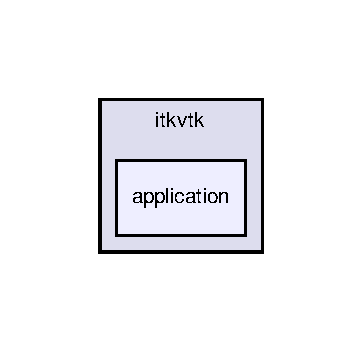
\includegraphics[width=174pt]{dir_ae7b6cf1d538706c4ed807fa4a0e933b_dep}
\end{center}
\end{figure}
\subsection*{Files}
\begin{DoxyCompactItemize}
\item 
file {\bfseries \_\-\_\-init\_\-\_\-.py}
\item 
file {\bfseries \_\-iterative\_\-watershed.py}
\item 
file {\bfseries auto\_\-watershed.py}
\item 
file {\bfseries gradient.py}
\item 
file {\bfseries smoothing.py}
\item 
file {\bfseries watershed.py}
\end{DoxyCompactItemize}

\hypertarget{dir_c5517966d86bcfb7cb507e4e9fa1040b}{
\section{/home/omaier/Programming/Python/medpy/src/medpy/application/ Directory Reference}
\label{dir_c5517966d86bcfb7cb507e4e9fa1040b}\index{/home/omaier/Programming/Python/medpy/src/medpy/application/ Directory Reference@{/home/omaier/Programming/Python/medpy/src/medpy/application/ Directory Reference}}
}
Directory dependency graph for /home/omaier/Programming/Python/medpy/src/medpy/application/:\nopagebreak
\begin{figure}[H]
\begin{center}
\leavevmode
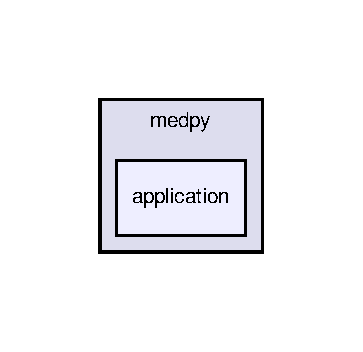
\includegraphics[width=174pt]{dir_c5517966d86bcfb7cb507e4e9fa1040b_dep}
\end{center}
\end{figure}
\subsection*{Files}
\begin{DoxyCompactItemize}
\item 
file {\bfseries \_\-\_\-init\_\-\_\-.py}
\item 
file {\bfseries \_\-label\_\-image\_\-statistics.py}
\item 
file {\bfseries \_\-old\_\-testbed\_\-regional\_\-term.py}
\item 
file {\bfseries \_\-watershed\_\-ift.py}
\item 
file {\bfseries count\_\-holes\_\-in\_\-rings.py}
\item 
file {\bfseries count\_\-labels.py}
\item 
file {\bfseries evaluate.py}
\item 
file {\bfseries extract\_\-mask\_\-position.py}
\item 
file {\bfseries extract\_\-min\_\-max.py}
\item 
file {\bfseries extract\_\-sub\_\-volume.py}
\item 
file {\bfseries extract\_\-sub\_\-volume\_\-by\_\-example.py}
\item 
file {\bfseries fouriertransformation.py}
\item 
file {\bfseries gradient.py}
\item 
file {\bfseries morphology.py}
\item 
file {\bfseries plotsuperposition.py}
\item 
file {\bfseries reduce.py}
\item 
file {\bfseries rt\_\-testbed\_\-creation.py}
\item 
file {\bfseries rt\_\-testbed\_\-histogram.py}
\item 
file {\bfseries rt\_\-testbed\_\-log.py}
\item 
file {\bfseries rt\_\-testbed\_\-visualize.py}
\item 
file {\bfseries superimposition.py}
\item 
file {\bfseries test.py}
\item 
file {\bfseries test2.py}
\item 
file {\bfseries testbed\_\-graphcut.py}
\item 
file {\bfseries testbed\_\-tamura.py}
\item 
file {\bfseries viscous\_\-eqsplit\_\-premorphology.py}
\item 
file {\bfseries viscous\_\-weighted\_\-premorphology.py}
\end{DoxyCompactItemize}

\hypertarget{dir_8cc032a1fcb6249cfe1ae3fdfbbf69e2}{
\section{/home/omaier/Programming/Python/medpy/src/medpy/core/ Directory Reference}
\label{dir_8cc032a1fcb6249cfe1ae3fdfbbf69e2}\index{/home/omaier/Programming/Python/medpy/src/medpy/core/ Directory Reference@{/home/omaier/Programming/Python/medpy/src/medpy/core/ Directory Reference}}
}
Directory dependency graph for /home/omaier/Programming/Python/medpy/src/medpy/core/:\nopagebreak
\begin{figure}[H]
\begin{center}
\leavevmode
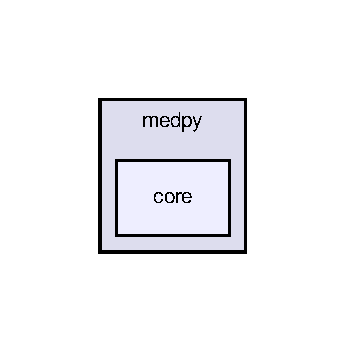
\includegraphics[width=166pt]{dir_8cc032a1fcb6249cfe1ae3fdfbbf69e2_dep}
\end{center}
\end{figure}
\subsection*{Files}
\begin{DoxyCompactItemize}
\item 
file {\bfseries \_\-\_\-init\_\-\_\-.py}
\item 
file {\bfseries exceptions.py}
\item 
file {\bfseries Logger.py}
\end{DoxyCompactItemize}

\hypertarget{dir_03a1cf7b93882f249938911ad428f675}{
\section{/home/omaier/Programming/Python/medpy/src/medpy/unittests/filter/ Directory Reference}
\label{dir_03a1cf7b93882f249938911ad428f675}\index{/home/omaier/Programming/Python/medpy/src/medpy/unittests/filter/ Directory Reference@{/home/omaier/Programming/Python/medpy/src/medpy/unittests/filter/ Directory Reference}}
}
Directory dependency graph for /home/omaier/Programming/Python/medpy/src/medpy/unittests/filter/:\nopagebreak
\begin{figure}[H]
\begin{center}
\leavevmode
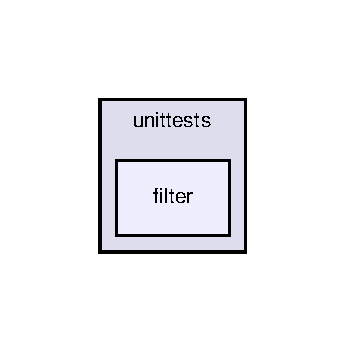
\includegraphics[width=166pt]{dir_03a1cf7b93882f249938911ad428f675_dep}
\end{center}
\end{figure}
\subsection*{Files}
\begin{DoxyCompactItemize}
\item 
file {\bfseries \_\-\_\-init\_\-\_\-.py}
\item 
file {\bfseries LabelImageStatistics.py}
\end{DoxyCompactItemize}

\hypertarget{dir_f5b35c2bce931702d8fae99875e74ac6}{
\section{/home/omaier/Programming/Python/medpy/src/medpy/filter/ Directory Reference}
\label{dir_f5b35c2bce931702d8fae99875e74ac6}\index{/home/omaier/Programming/Python/medpy/src/medpy/filter/ Directory Reference@{/home/omaier/Programming/Python/medpy/src/medpy/filter/ Directory Reference}}
}
Directory dependency graph for /home/omaier/Programming/Python/medpy/src/medpy/filter/:\nopagebreak
\begin{figure}[H]
\begin{center}
\leavevmode
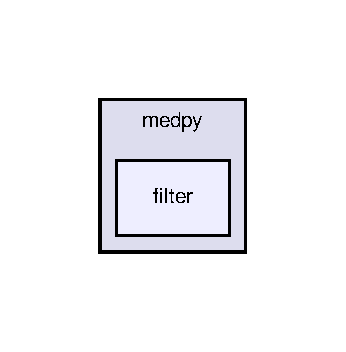
\includegraphics[width=166pt]{dir_f5b35c2bce931702d8fae99875e74ac6_dep}
\end{center}
\end{figure}
\subsection*{Files}
\begin{DoxyCompactItemize}
\item 
file {\bfseries \_\-\_\-init\_\-\_\-.py}
\item 
file {\bfseries \_\-FitLabelsToMask.py}
\item 
file {\bfseries AnisotropicDiffusion.py}
\item 
file {\bfseries label.py}
\item 
file {\bfseries LabelImageStatistics.py}
\item 
file {\bfseries MinimaExtraction.py}
\item 
file {\bfseries Watershed.py}
\end{DoxyCompactItemize}

\hypertarget{dir_bd5d33f2c5954a2eebdd47f5077338f3}{
\section{/home/omaier/Programming/Python/medpy/src/medpy/unittests/graphcut/ Directory Reference}
\label{dir_bd5d33f2c5954a2eebdd47f5077338f3}\index{/home/omaier/Programming/Python/medpy/src/medpy/unittests/graphcut/ Directory Reference@{/home/omaier/Programming/Python/medpy/src/medpy/unittests/graphcut/ Directory Reference}}
}
Directory dependency graph for /home/omaier/Programming/Python/medpy/src/medpy/unittests/graphcut/:\nopagebreak
\begin{figure}[H]
\begin{center}
\leavevmode
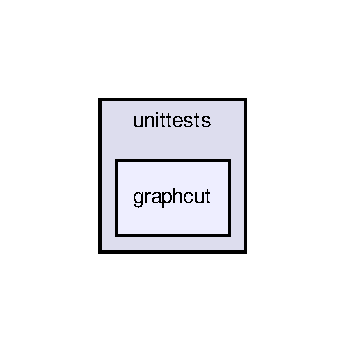
\includegraphics[width=166pt]{dir_bd5d33f2c5954a2eebdd47f5077338f3_dep}
\end{center}
\end{figure}
\subsection*{Files}
\begin{DoxyCompactItemize}
\item 
file {\bfseries \_\-\_\-init\_\-\_\-.py}
\item 
file {\bfseries energy.py}
\item 
file {\bfseries generatecut.py}
\item 
file {\bfseries graph.py}
\item 
file {\bfseries parse.py}
\item 
file {\bfseries pipeline.py}
\end{DoxyCompactItemize}

\hypertarget{dir_59c3afa8d11d678041e98ae320c1dfd8}{
\section{/home/omaier/Programming/Python/medpy/src/medpy/graphcut/ Directory Reference}
\label{dir_59c3afa8d11d678041e98ae320c1dfd8}\index{/home/omaier/Programming/Python/medpy/src/medpy/graphcut/ Directory Reference@{/home/omaier/Programming/Python/medpy/src/medpy/graphcut/ Directory Reference}}
}
Directory dependency graph for /home/omaier/Programming/Python/medpy/src/medpy/graphcut/:\nopagebreak
\begin{figure}[H]
\begin{center}
\leavevmode
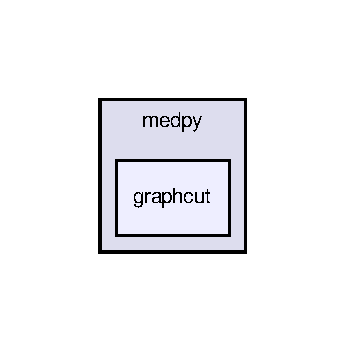
\includegraphics[width=166pt]{dir_59c3afa8d11d678041e98ae320c1dfd8_dep}
\end{center}
\end{figure}
\subsection*{Files}
\begin{DoxyCompactItemize}
\item 
file {\bfseries \_\-\_\-init\_\-\_\-.py}
\item 
file {\bfseries energy\_\-label.py}
\item 
file {\bfseries energy\_\-voxel.py}
\item 
file {\bfseries generate.py}
\item 
file {\bfseries graph.py}
\item 
file {\bfseries write.py}
\end{DoxyCompactItemize}

\hypertarget{dir_a11a37e7adb08f63603dd4321274f18e}{
\section{/home/omaier/Programming/Python/medpy/src/medpy/io/ Directory Reference}
\label{dir_a11a37e7adb08f63603dd4321274f18e}\index{/home/omaier/Programming/Python/medpy/src/medpy/io/ Directory Reference@{/home/omaier/Programming/Python/medpy/src/medpy/io/ Directory Reference}}
}
Directory dependency graph for /home/omaier/Programming/Python/medpy/src/medpy/io/:\nopagebreak
\begin{figure}[H]
\begin{center}
\leavevmode
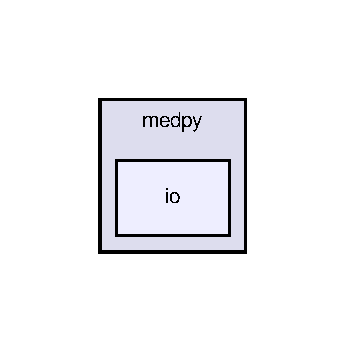
\includegraphics[width=166pt]{dir_a11a37e7adb08f63603dd4321274f18e_dep}
\end{center}
\end{figure}
\subsection*{Files}
\begin{DoxyCompactItemize}
\item 
file {\bfseries \_\-\_\-init\_\-\_\-.py}
\end{DoxyCompactItemize}

\hypertarget{dir_6b2c9baf6b61af08aa073b84d71c19d6}{
\section{/home/omaier/Programming/Python/medpy/src/medpy/itkvtk/ Directory Reference}
\label{dir_6b2c9baf6b61af08aa073b84d71c19d6}\index{/home/omaier/Programming/Python/medpy/src/medpy/itkvtk/ Directory Reference@{/home/omaier/Programming/Python/medpy/src/medpy/itkvtk/ Directory Reference}}
}
Directory dependency graph for /home/omaier/Programming/Python/medpy/src/medpy/itkvtk/:\nopagebreak
\begin{figure}[H]
\begin{center}
\leavevmode
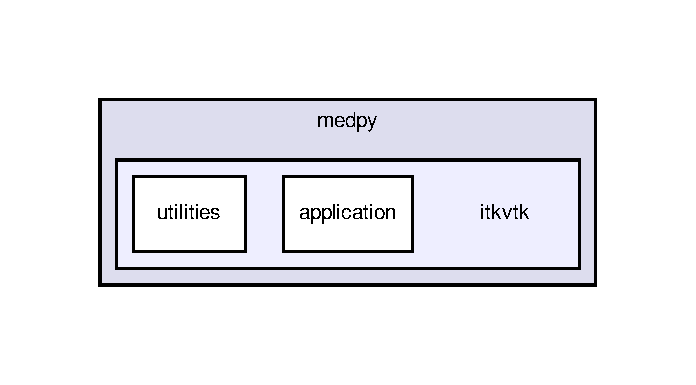
\includegraphics[width=334pt]{dir_6b2c9baf6b61af08aa073b84d71c19d6_dep}
\end{center}
\end{figure}
\subsection*{Directories}
\begin{DoxyCompactItemize}
\item 
directory \hyperlink{dir_ae7b6cf1d538706c4ed807fa4a0e933b}{application}
\item 
directory \hyperlink{dir_e7002451b424f64dcea7a554c3342e35}{utilities}
\end{DoxyCompactItemize}
\subsection*{Files}
\begin{DoxyCompactItemize}
\item 
file {\bfseries \_\-\_\-init\_\-\_\-.py}
\end{DoxyCompactItemize}

\hypertarget{dir_38eb81983c5e08a00adc0664db29ada6}{
\section{/home/omaier/Programming/Python/medpy/src/medpy/ Directory Reference}
\label{dir_38eb81983c5e08a00adc0664db29ada6}\index{/home/omaier/Programming/Python/medpy/src/medpy/ Directory Reference@{/home/omaier/Programming/Python/medpy/src/medpy/ Directory Reference}}
}
Directory dependency graph for /home/omaier/Programming/Python/medpy/src/medpy/:\nopagebreak
\begin{figure}[H]
\begin{center}
\leavevmode
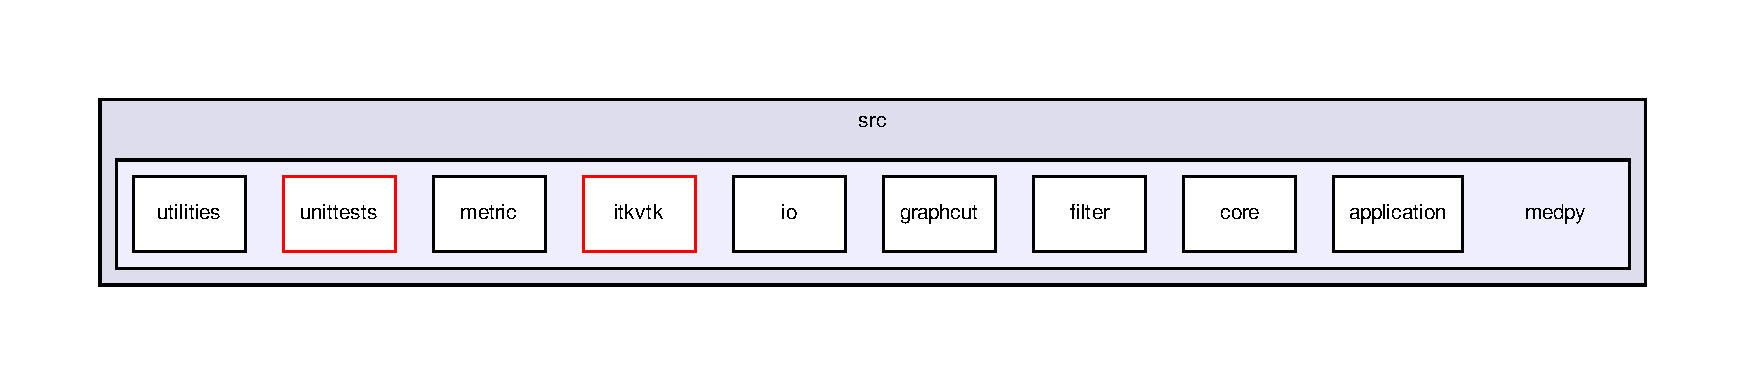
\includegraphics[width=400pt]{dir_38eb81983c5e08a00adc0664db29ada6_dep}
\end{center}
\end{figure}
\subsection*{Directories}
\begin{DoxyCompactItemize}
\item 
directory \hyperlink{dir_068fda1acee30f0af139aaae1e62455f}{\_\-graphcut}
\item 
directory \hyperlink{dir_c5517966d86bcfb7cb507e4e9fa1040b}{application}
\item 
directory \hyperlink{dir_8cc032a1fcb6249cfe1ae3fdfbbf69e2}{core}
\item 
directory \hyperlink{dir_5f01a90212dd9f41f27f8e065966fb0e}{features}
\item 
directory \hyperlink{dir_f5b35c2bce931702d8fae99875e74ac6}{filter}
\item 
directory \hyperlink{dir_59c3afa8d11d678041e98ae320c1dfd8}{graphcut}
\item 
directory \hyperlink{dir_a11a37e7adb08f63603dd4321274f18e}{io}
\item 
directory \hyperlink{dir_6b2c9baf6b61af08aa073b84d71c19d6}{itkvtk}
\item 
directory \hyperlink{dir_ba0d92d5a0f4019f24a5497855281ca9}{metric}
\item 
directory \hyperlink{dir_0c68ac67082dc79494ca6fb791a56297}{unittests}
\item 
directory \hyperlink{dir_361eb00c2881437ffc5ae8a4f7f3c1d3}{utilities}
\end{DoxyCompactItemize}
\subsection*{Files}
\begin{DoxyCompactItemize}
\item 
file {\bfseries \_\-\_\-init\_\-\_\-.py}
\end{DoxyCompactItemize}

\hypertarget{dir_91c04c4eef682b0235d3fdf5640d8ecc}{
\section{/home/omaier/Programming/Python/medpy/src/medpy/unittests/metric/ Directory Reference}
\label{dir_91c04c4eef682b0235d3fdf5640d8ecc}\index{/home/omaier/Programming/Python/medpy/src/medpy/unittests/metric/ Directory Reference@{/home/omaier/Programming/Python/medpy/src/medpy/unittests/metric/ Directory Reference}}
}
Directory dependency graph for /home/omaier/Programming/Python/medpy/src/medpy/unittests/metric/:\nopagebreak
\begin{figure}[H]
\begin{center}
\leavevmode
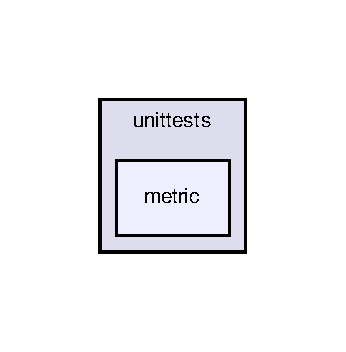
\includegraphics[width=166pt]{dir_91c04c4eef682b0235d3fdf5640d8ecc_dep}
\end{center}
\end{figure}
\subsection*{Files}
\begin{DoxyCompactItemize}
\item 
file {\bfseries \_\-\_\-init\_\-\_\-.py}
\item 
file {\bfseries Surface.py}
\item 
file {\bfseries Volume.py}
\end{DoxyCompactItemize}

\hypertarget{dir_ba0d92d5a0f4019f24a5497855281ca9}{
\section{/home/omaier/Programming/Python/medpy/src/medpy/metric/ Directory Reference}
\label{dir_ba0d92d5a0f4019f24a5497855281ca9}\index{/home/omaier/Programming/Python/medpy/src/medpy/metric/ Directory Reference@{/home/omaier/Programming/Python/medpy/src/medpy/metric/ Directory Reference}}
}
Directory dependency graph for /home/omaier/Programming/Python/medpy/src/medpy/metric/:\nopagebreak
\begin{figure}[H]
\begin{center}
\leavevmode
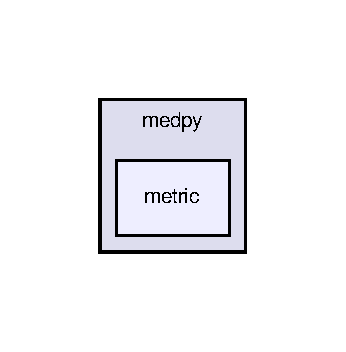
\includegraphics[width=166pt]{dir_ba0d92d5a0f4019f24a5497855281ca9_dep}
\end{center}
\end{figure}
\subsection*{Files}
\begin{DoxyCompactItemize}
\item 
file {\bfseries \_\-\_\-init\_\-\_\-.py}
\item 
file {\bfseries histogram.py}
\item 
file {\bfseries surface.py}
\item 
file {\bfseries volume.py}
\end{DoxyCompactItemize}

\hypertarget{dir_39b96f9c4012765d2b281918e9f3d34d}{
\section{/home/omaier/Programming/Python/medpy/src/ Directory Reference}
\label{dir_39b96f9c4012765d2b281918e9f3d34d}\index{/home/omaier/Programming/Python/medpy/src/ Directory Reference@{/home/omaier/Programming/Python/medpy/src/ Directory Reference}}
}
Directory dependency graph for /home/omaier/Programming/Python/medpy/src/:\nopagebreak
\begin{figure}[H]
\begin{center}
\leavevmode
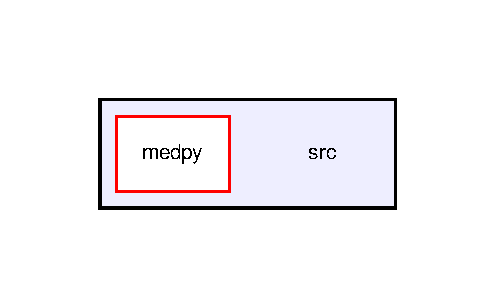
\includegraphics[width=238pt]{dir_39b96f9c4012765d2b281918e9f3d34d_dep}
\end{center}
\end{figure}
\subsection*{Directories}
\begin{DoxyCompactItemize}
\item 
directory \hyperlink{dir_38eb81983c5e08a00adc0664db29ada6}{medpy}
\end{DoxyCompactItemize}

\hypertarget{dir_0c68ac67082dc79494ca6fb791a56297}{
\section{/home/omaier/Programming/Python/medpy/src/medpy/unittests/ Directory Reference}
\label{dir_0c68ac67082dc79494ca6fb791a56297}\index{/home/omaier/Programming/Python/medpy/src/medpy/unittests/ Directory Reference@{/home/omaier/Programming/Python/medpy/src/medpy/unittests/ Directory Reference}}
}
Directory dependency graph for /home/omaier/Programming/Python/medpy/src/medpy/unittests/:\nopagebreak
\begin{figure}[H]
\begin{center}
\leavevmode
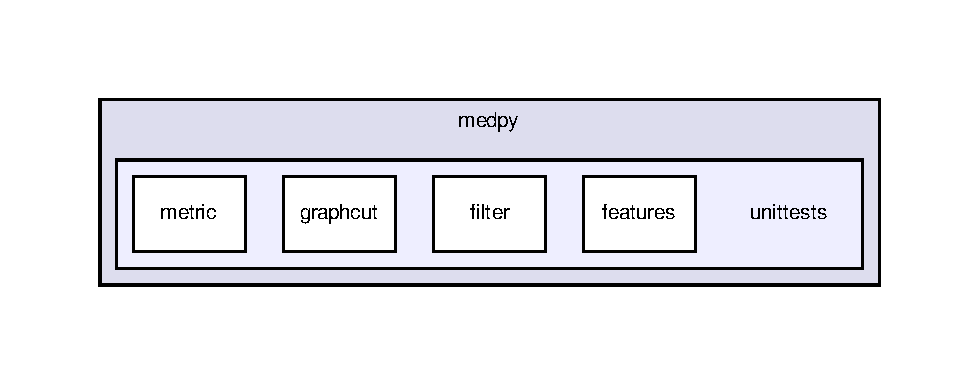
\includegraphics[width=400pt]{dir_0c68ac67082dc79494ca6fb791a56297_dep}
\end{center}
\end{figure}
\subsection*{Directories}
\begin{DoxyCompactItemize}
\item 
directory \hyperlink{dir_1a6919a091e2f65aa96961fed604a360}{features}
\item 
directory \hyperlink{dir_03a1cf7b93882f249938911ad428f675}{filter}
\item 
directory \hyperlink{dir_bd5d33f2c5954a2eebdd47f5077338f3}{graphcut}
\item 
directory \hyperlink{dir_91c04c4eef682b0235d3fdf5640d8ecc}{metric}
\end{DoxyCompactItemize}
\subsection*{Files}
\begin{DoxyCompactItemize}
\item 
file {\bfseries \_\-\_\-init\_\-\_\-.py}
\item 
file {\bfseries run.py}
\end{DoxyCompactItemize}

\hypertarget{dir_361eb00c2881437ffc5ae8a4f7f3c1d3}{
\section{/home/omaier/Programming/Python/medpy/src/medpy/utilities/ Directory Reference}
\label{dir_361eb00c2881437ffc5ae8a4f7f3c1d3}\index{/home/omaier/Programming/Python/medpy/src/medpy/utilities/ Directory Reference@{/home/omaier/Programming/Python/medpy/src/medpy/utilities/ Directory Reference}}
}
Directory dependency graph for /home/omaier/Programming/Python/medpy/src/medpy/utilities/:\nopagebreak
\begin{figure}[H]
\begin{center}
\leavevmode
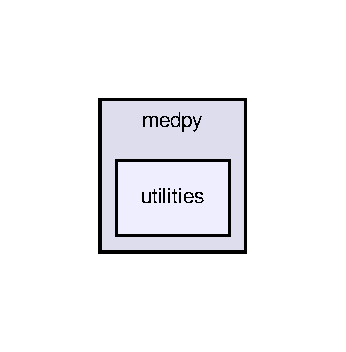
\includegraphics[width=166pt]{dir_361eb00c2881437ffc5ae8a4f7f3c1d3_dep}
\end{center}
\end{figure}
\subsection*{Files}
\begin{DoxyCompactItemize}
\item 
file {\bfseries \_\-\_\-init\_\-\_\-.py}
\item 
file {\bfseries nibabel.py}
\end{DoxyCompactItemize}

\hypertarget{dir_e7002451b424f64dcea7a554c3342e35}{
\section{/home/omaier/Programming/Python/medpy/src/medpy/itkvtk/utilities/ Directory Reference}
\label{dir_e7002451b424f64dcea7a554c3342e35}\index{/home/omaier/Programming/Python/medpy/src/medpy/itkvtk/utilities/ Directory Reference@{/home/omaier/Programming/Python/medpy/src/medpy/itkvtk/utilities/ Directory Reference}}
}
Directory dependency graph for /home/omaier/Programming/Python/medpy/src/medpy/itkvtk/utilities/:\nopagebreak
\begin{figure}[H]
\begin{center}
\leavevmode
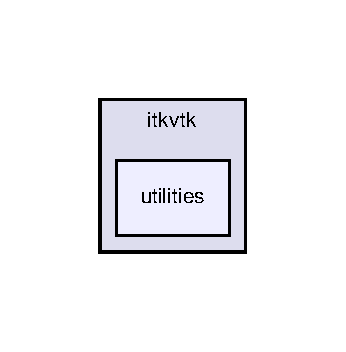
\includegraphics[width=166pt]{dir_e7002451b424f64dcea7a554c3342e35_dep}
\end{center}
\end{figure}
\subsection*{Files}
\begin{DoxyCompactItemize}
\item 
file {\bfseries \_\-\_\-init\_\-\_\-.py}
\item 
file {\bfseries itku.py}
\item 
file {\bfseries vtku.py}
\end{DoxyCompactItemize}

\chapter{Namespace Documentation}
\hypertarget{namespacemedpy_1_1graphcut}{
\section{Package medpy.graphcut}
\label{namespacemedpy_1_1graphcut}\index{medpy.graphcut@{medpy.graphcut}}
}


Functionalities to use graph-\/cut (max-\/flow/min-\/cut) algorithms.  


\subsection*{Packages}
\begin{DoxyCompactItemize}
\item 
package \hyperlink{namespacemedpy_1_1graphcut_1_1cut}{cut}


\begin{DoxyCompactList}\small\item\em Prepares, compiles and executed graph-\/cut implementations using the graphs created by the graph module of this package. \end{DoxyCompactList}

\item 
package \hyperlink{namespacemedpy_1_1graphcut_1_1energy}{energy}


\begin{DoxyCompactList}\small\item\em Run-\/time optimized energy functions for graph-\/cut. \end{DoxyCompactList}

\item 
package \hyperlink{namespacemedpy_1_1graphcut_1_1generate}{generate}


\begin{DoxyCompactList}\small\item\em Generates output files from graphs that are processable by graph-\/cut algorithms. \end{DoxyCompactList}

\item 
package \hyperlink{namespacemedpy_1_1graphcut_1_1graph}{graph}


\begin{DoxyCompactList}\small\item\em Create and modify graphs from nD label-\/images to be used in graph-\/cut algorithms. \end{DoxyCompactList}

\item 
package \hyperlink{namespacemedpy_1_1graphcut_1_1parse}{parse}


\begin{DoxyCompactList}\small\item\em Parses the output returned by graph-\/cut implementations. \end{DoxyCompactList}

\item 
package \hyperlink{namespacemedpy_1_1graphcut_1_1write}{write}


\begin{DoxyCompactList}\small\item\em Functions to persist a graph in various file formats. \end{DoxyCompactList}

\end{DoxyCompactItemize}
\subsection*{Variables}
\begin{DoxyCompactItemize}
\item 
\hypertarget{namespacemedpy_1_1graphcut_aad412f9af7e17894cc03632be5905a54}{
list {\bfseries \_\-\_\-all\_\-\_\-} = \mbox{[}$\,$\mbox{]}}
\label{namespacemedpy_1_1graphcut_aad412f9af7e17894cc03632be5905a54}

\end{DoxyCompactItemize}


\subsection{Detailed Description}
Functionalities to use graph-\/cut (max-\/flow/min-\/cut) algorithms. Provides methods to build graphs from label-\/image using arbitrary energy functions (boundary and regional terms), format these graphs to be processed by a number of graph-\/cut implementations, executing these and parsing the results.

Supported graph-\/cut algorithms with tested version number:\par

\begin{DoxyItemize}
\item {\bfseries BK\_\-MFMC:} Boykov and Kolmogorovs (1) max-\/flow/min-\/cut C++ implementation (a) \mbox{[}v3.01\mbox{]}
\end{DoxyItemize}

Modules:
\begin{DoxyItemize}
\item graph: Create and modify graphs from nD label-\/images to be used in graph-\/cut algorithms.
\item generate: Generates output files from graphs that are processable by graph-\/cut algorithms.
\item cut: Prepares, compiles and executed graph-\/cut implementations.
\item parse: Parses the output returned by graph-\/cut implementations.
\item energy: Run-\/time optimized energy functions for graph-\/cut.
\end{DoxyItemize}

\begin{DoxyNote}{Note}
This package makes use of  medpy.core.Logger to generate progress and debug messages.
\end{DoxyNote}
(a) \href{http://vision.csd.uwo.ca/code/}{\tt http://vision.csd.uwo.ca/code/} \mbox{[}last seen: 01/2012\mbox{]}

(1) Boykov Y., Kolmogorov V. / \char`\"{}An Experimental Comparison of Min-\/Cut/Max-\/Flow
 Algorithms for Energy Minimization in Vision\char`\"{} / In IEEE Transactions on PAMI, Vol. 26, No. 9, pp. 1124-\/1137, Sept. 2004

Provides functionalities to efficiently construct graphs from various sources using arbitrary energy functions (boundary and regional terms). The graph can then be saved in the Dimacs graph standard and/or processed (i.e. cut) using 3rd party graph-\/cut algorithms.

Supported graph-\/cut algorithms with tested version number:\par

\begin{DoxyItemize}
\item {\bfseries BK\_\-MFMC:} Boykov and Kolmogorovs (1) max-\/flow/min-\/cut C++ implementation (a) \mbox{[}v3.01\mbox{]}
\end{DoxyItemize}

Modules:
\begin{DoxyItemize}
\item graph: The basic Graph object.
\item write: Functions to persist a graph in various file formats like Dimacs (b).
\item maxflow: C++ wrapper around the max-\/flow/min-\/cut implementation of (1)
\item generate: Provides functions to generate graphs efficiently from nD label-\/images.
\item energy: Run-\/time optimized energy functions for the graph generation.
\end{DoxyItemize}

\begin{DoxyNote}{Note}
This package makes use of  medpy.core.Logger to generate progress and debug messages.
\end{DoxyNote}
(a) \href{http://vision.csd.uwo.ca/code/}{\tt http://vision.csd.uwo.ca/code/} \mbox{[}last seen: 01/2012\mbox{]} (b) \href{http://lpsolve.sourceforge.net/5.5/DIMACS_maxf.htm}{\tt http://lpsolve.sourceforge.net/5.5/DIMACS\_\-maxf.htm}

(1) Boykov Y., Kolmogorov V. / \char`\"{}An Experimental Comparison of Min-\/Cut/Max-\/Flow
 Algorithms for Energy Minimization in Vision\char`\"{} / In IEEE Transactions on PAMI, Vol. 26, No. 9, pp. 1124-\/1137, Sept. 2004

\begin{DoxyAuthor}{Author}
Oskar Maier 
\end{DoxyAuthor}

\hypertarget{namespacemedpy_1_1graphcut_1_1cut}{
\section{Package medpy.graphcut.cut}
\label{namespacemedpy_1_1graphcut_1_1cut}\index{medpy.graphcut.cut@{medpy.graphcut.cut}}
}


Prepares, compiles and executed graph-\/cut implementations using the graphs created by the graph module of this package.  




\subsection{Detailed Description}
Prepares, compiles and executed graph-\/cut implementations using the graphs created by the graph module of this package. Note that the functionality provided by this module depends highly on the platform, the availability of 3rd party tools and executes foreign code. It should only be used when completely understood. Otherwise manual execution of this step is preferable.

All functions in this module are highly depend on the actual implementation of the graph-\/cut algorithm they are intended to be used for. They require a minimal version number and it can not be ensured, that they will work with other versions.

See the package description for a list of the supported graph-\/cut implementations.

Functions:
\begin{DoxyItemize}
\item def bk\_\-mfmc\_\-cut(source\_\-file, gpp\_\-location = False): Execute a graph cut using Boyov and Kolmogorovs max-\/flow/min-\/cut algorithm.
\end{DoxyItemize}

\begin{DoxyAuthor}{Author}
Oskar Maier 
\end{DoxyAuthor}
\begin{DoxyVersion}{Version}
d0.1.0 
\end{DoxyVersion}
\begin{DoxySince}{Since}
2012-\/01-\/18  Development 
\end{DoxySince}

\hypertarget{namespacemedpy_1_1graphcut_1_1energy}{
\section{Package medpy.graphcut.energy}
\label{namespacemedpy_1_1graphcut_1_1energy}\index{medpy.graphcut.energy@{medpy.graphcut.energy}}
}


Run-\/time optimized energy functions for graph-\/cut.  


\subsection*{Functions}
\begin{DoxyCompactItemize}
\item 
def \hyperlink{namespacemedpy_1_1graphcut_1_1energy_a2bf88e97c3a4d86bfa293ead5bdefb33}{boundary\_\-stawiaski}
\begin{DoxyCompactList}\small\item\em An implementation of the boundary term in (1), suitable to be used with the \hyperlink{}{function. }\end{DoxyCompactList}\end{DoxyCompactItemize}


\subsection{Detailed Description}
Run-\/time optimized energy functions for graph-\/cut. Provides a number of standard energy functions for both, boundary and regional terms, that follow the signature required for building graphs using the graph module of this package. Additionally a number of convenience functions for re-\/occurring data processing are given.

Functions:
\begin{DoxyItemize}
\item def boundary\_\-stawiaski(label\_\-image, r1\_\-bb, r2\_\-bb, r1\_\-id, r2\_\-id, (gradient\_\-image)): boundary term implementation in (1)
\end{DoxyItemize}

(1) Stawiaski J., Decenciere E., Bidlaut F. / \char`\"{}Interactive Liver Tumor Segmentation
 Using Graph-\/cuts and watershed\char`\"{} / MICCAI 2008 participation

\begin{DoxyAuthor}{Author}
Oskar Maier 
\end{DoxyAuthor}
\begin{DoxyVersion}{Version}
d0.1.0 
\end{DoxyVersion}
\begin{DoxySince}{Since}
2012-\/01-\/18  Development
\end{DoxySince}
Provides a number of standard energy functions for both, boundary and regional terms, that follow the signature required for building graphs using the graph module of this package. Additionally a number of convenience functions for re-\/occurring data processing are given.

Functions:
\begin{DoxyItemize}
\item def boundary\_\-stawiaski(label\_\-image, (gradient\_\-image)): boundary term implementation in (1)
\end{DoxyItemize}

(1) Stawiaski J., Decenciere E., Bidlaut F. / \char`\"{}Interactive Liver Tumor Segmentation
 Using Graph-\/cuts and watershed\char`\"{} / MICCAI 2008 participation

\begin{DoxyAuthor}{Author}
Oskar Maier 
\end{DoxyAuthor}
\begin{DoxyVersion}{Version}
d0.1.0 
\end{DoxyVersion}
\begin{DoxySince}{Since}
2012-\/01-\/18  Development 
\end{DoxySince}


\subsection{Function Documentation}
\hypertarget{namespacemedpy_1_1graphcut_1_1energy_a2bf88e97c3a4d86bfa293ead5bdefb33}{
\index{medpy::graphcut::energy@{medpy::graphcut::energy}!boundary\_\-stawiaski@{boundary\_\-stawiaski}}
\index{boundary\_\-stawiaski@{boundary\_\-stawiaski}!medpy::graphcut::energy@{medpy::graphcut::energy}}
\subsubsection[{boundary\_\-stawiaski}]{\setlength{\rightskip}{0pt plus 5cm}def medpy.graphcut.energy.boundary\_\-stawiaski (
\begin{DoxyParamCaption}
\item[{}]{label\_\-image, }
\item[{}]{gradient\_\-image}
\end{DoxyParamCaption}
)}}
\label{namespacemedpy_1_1graphcut_1_1energy_a2bf88e97c3a4d86bfa293ead5bdefb33}


An implementation of the boundary term in (1), suitable to be used with the \hyperlink{}{function. }

Determines for each two supplied regions the voxels forming their border assuming ndim$\ast$2-\/connectedness (e.g. 3$\ast$2=6 for 3D). From the gradient magnitude values of each end-\/point voxel the border-\/voxel pairs, the highest one is selected and passed to a strictly positive and decreasing function g, which is defined as: \[ g(x) = \left(\frac{1}{1+|x|}\right)^k \] ,where $k=2$. The final weight $w_{i,j}$ between two regions $r_i$ and $r_j$ is then determined by the sum of all these neighbour values: \[ w = \sum_{e_{m,n}|inF_{(r_i,r_j)}}g(\max(|I(m)|,|I(n)|)) \] , where $F_{(r_i,r_j)}$ is the set of border voxel-\/pairs $e_{m,n}$ between the regions $r_i$ and $r_j$ and $|I(p)|$ the absolute of the gradient magnitude at the voxel $p$

This boundary\_\-function works as an edge indicator in the original image. In simpler words the weight (and therefore the energy) is obtained by summing the local contrast along the boundaries between two regions.

\begin{DoxyNote}{Note}
This function requires the gradient magnitude image of the original image to be passed along. That means that \hyperlink{}{has to be called with boundary\_\-term\_\-args set to the gradient image.   label\_\-image the label image  label\_\-image numpy.ndarray  gradient\_\-image The gradient magnitude image of the original image.  gradient\_\-image numpy.ndarray   a dictionary with the edges as keys and the respective weight tuples as values  dict }
\end{DoxyNote}


Definition at line 72 of file energy.py.


\hypertarget{namespacemedpy_1_1graphcut_1_1generate}{
\section{Package medpy.graphcut.generate}
\label{namespacemedpy_1_1graphcut_1_1generate}\index{medpy.graphcut.generate@{medpy.graphcut.generate}}
}


Generates output files from graphs that are processable by graph-\/cut algorithms.  


\subsection*{Functions}
\begin{DoxyCompactItemize}
\item 
def \hyperlink{namespacemedpy_1_1graphcut_1_1generate_a5533013ae970ceb90ca67cf4e6f1da41}{graph\_\-from\_\-voxels}
\begin{DoxyCompactList}\small\item\em Create a \hyperlink{classmedpy_1_1graphcut_1_1graph_1_1Graph}{graphcut.graph.Graph} object for all voxels of an image with a ndim $\ast$ 2 neighbourhood. \end{DoxyCompactList}\item 
def \hyperlink{namespacemedpy_1_1graphcut_1_1generate_a137ecdeeb31eb5be7bdcf70da1509477}{graph\_\-from\_\-labels}
\begin{DoxyCompactList}\small\item\em Create a \hyperlink{classmedpy_1_1graphcut_1_1graph_1_1Graph}{graphcut.graph.Graph} object from a nD label image. \end{DoxyCompactList}\end{DoxyCompactItemize}


\subsection{Detailed Description}
Generates output files from graphs that are processable by graph-\/cut algorithms. Provides functionality to generate graphs efficiently from nD label-\/images and image voxels.

All functions in this module are highly depend on the actual implementation of the graph-\/cut algorithm they are intended to be used for. They require a minimal version number and it can not be ensured, that they will work with other versions.

See the package description for a list of the supported graph-\/cut implementations.

Functions:
\begin{DoxyItemize}
\item def bk\_\-mfmc\_\-generate(graph): Generate a C++ file for Boyov and Kolmogorovs max-\/flow/min-\/cut algorithm.
\end{DoxyItemize}

\begin{DoxyAuthor}{Author}
Oskar Maier 
\end{DoxyAuthor}
\begin{DoxyVersion}{Version}
d0.1.0 
\end{DoxyVersion}
\begin{DoxySince}{Since}
2012-\/01-\/18  Development
\end{DoxySince}
Functions:
\begin{DoxyItemize}
\item def graph\_\-from\_\-labels(label\_\-image, fg\_\-markers, bg\_\-markers, regional\_\-term = False, boundary\_\-term = False, regional\_\-term\_\-args = False, boundary\_\-term\_\-args = False): Creates a Graph object from a nD label image.
\item def graph\_\-from\_\-voxels(fg\_\-markers, bg\_\-markers, regional\_\-term = False, boundary\_\-term = False, regional\_\-term\_\-args = False, boundary\_\-term\_\-args = False): Creates a Graph object from the voxels of an image. \begin{DoxyAuthor}{Author}
Oskar Maier 
\end{DoxyAuthor}
\begin{DoxyVersion}{Version}
r0.2.0 
\end{DoxyVersion}
\begin{DoxySince}{Since}
2012-\/01-\/18  Release 
\end{DoxySince}

\end{DoxyItemize}

\subsection{Function Documentation}
\hypertarget{namespacemedpy_1_1graphcut_1_1generate_a137ecdeeb31eb5be7bdcf70da1509477}{
\index{medpy::graphcut::generate@{medpy::graphcut::generate}!graph\_\-from\_\-labels@{graph\_\-from\_\-labels}}
\index{graph\_\-from\_\-labels@{graph\_\-from\_\-labels}!medpy::graphcut::generate@{medpy::graphcut::generate}}
\subsubsection[{graph\_\-from\_\-labels}]{\setlength{\rightskip}{0pt plus 5cm}def medpy.graphcut.generate.graph\_\-from\_\-labels (
\begin{DoxyParamCaption}
\item[{}]{label\_\-image, }
\item[{}]{fg\_\-markers, }
\item[{}]{bg\_\-markers, }
\item[{}]{regional\_\-term = {\ttfamily False}, }
\item[{}]{boundary\_\-term = {\ttfamily False}, }
\item[{}]{regional\_\-term\_\-args = {\ttfamily False}, }
\item[{}]{boundary\_\-term\_\-args = {\ttfamily False}}
\end{DoxyParamCaption}
)}}
\label{namespacemedpy_1_1graphcut_1_1generate_a137ecdeeb31eb5be7bdcf70da1509477}


Create a \hyperlink{classmedpy_1_1graphcut_1_1graph_1_1Graph}{graphcut.graph.Graph} object from a nD label image. 

Every region of the label image is regarded as a node. They are connected to their immediate neighbours by arcs. If to regions are neighbours is determined using ndim$\ast$2-\/connectedness (e.g. 3$\ast$2=6 for 3D). In the next step the arcs weights (n-\/weights) are computed using the supplied boundary\_\-term function.

Implicitly the graph holds two additional nodes: the source and the sink, so called terminal nodes. These are connected with all other nodes through arcs of an initial weight (t-\/weight) of zero. All regions that are under the foreground markers are considered to be tightly bound to the source: The t-\/weight of the arc from source to these nodes is set to a maximum value. The same goes for the background markers: The covered regions receive a maximum (graphcut.graph.Graph.MAX) t-\/weight for their arc towards the sink.

\begin{DoxyNote}{Note}
If a region is marked as both, foreground and background, the background marker is given higher priority.

all arcs whose weight is not explicitly set are assumed to carry a weight of zero.
\end{DoxyNote}

\begin{DoxyParams}{Parameters}
{\em label\_\-image} & The label image as an array containing uint values. Note that the region labels have to start from 1 and be continuous (\hyperlink{namespacemedpy_1_1filter_1_1label_abfba87c8b8fb3f0fb0e311dc90b20fba}{filter.label.relabel()}).  label\_\-image numpy.ndarray \\
\hline
{\em fg\_\-markers} & The foreground markers as binary array of the same shape as the label image.  fg\_\-markers ndarray \\
\hline
{\em bg\_\-markers} & The background markers as binary array of the same shape as the label image.  bg\_\-markers ndarray \\
\hline
{\em regional\_\-term} & This can be either False -\/ all t-\/weights are set to 0, except for the nodes that are directly connected to the source or sink. , or a function -\/ The supplied function is used to compute the t\_\-edges. It has to have the following signature regional\_\-term(label\_\-image, regions, bounding\_\-boxes, regional\_\-term\_\-args), and is supposed to return a dictionary with region-\/ids as keys and a tuple (source\_\-t\_\-weight, sink\_\-t\_\-weight) as values. The returned dictionary does only need to contain entries for nodes where one of the t-\/weights is not zero. Additional parameters can be passed via the regional\_\-term\_\-args argument.  regional\_\-term function \\
\hline
{\em boundary\_\-term} & This can be either False -\/ In which case the weight of all n\_\-edges i.e. between all nodes that are not source or sink, are set to 0. , or a function -\/ In which case it is used to compute the edges weights. The supplied function has to have the following signature fun(label\_\-image, boundary\_\-term\_\-args), and is supposed to return a dictionary with the graphs edges as keys and their n-\/weights as values. These weights are tuples of numbers assigning the weights in both directions of the edge. Additional parameters can be passed via the boundary\_\-term\_\-args argument.  boundary\_\-term function \\
\hline
{\em regional\_\-term\_\-args} & Use this to pass some additional parameters to the regional\_\-term function. \\
\hline
{\em boundary\_\-term\_\-args} & Use this to pass some additional parameters to the boundary\_\-term function.\\
\hline
\end{DoxyParams}
\begin{DoxyReturn}{Returns}
the created graph  \hyperlink{classmedpy_1_1graphcut_1_1graph_1_1Graph}{graphcut.graph.Graph}
\end{DoxyReturn}
AttributeError If an argument is maleformed.  FunctionError If one of the supplied functions returns unexpected results. 

Definition at line 227 of file generate.py.

\hypertarget{namespacemedpy_1_1graphcut_1_1generate_a5533013ae970ceb90ca67cf4e6f1da41}{
\index{medpy::graphcut::generate@{medpy::graphcut::generate}!graph\_\-from\_\-voxels@{graph\_\-from\_\-voxels}}
\index{graph\_\-from\_\-voxels@{graph\_\-from\_\-voxels}!medpy::graphcut::generate@{medpy::graphcut::generate}}
\subsubsection[{graph\_\-from\_\-voxels}]{\setlength{\rightskip}{0pt plus 5cm}def medpy.graphcut.generate.graph\_\-from\_\-voxels (
\begin{DoxyParamCaption}
\item[{}]{fg\_\-markers, }
\item[{}]{bg\_\-markers, }
\item[{}]{regional\_\-term = {\ttfamily False}, }
\item[{}]{boundary\_\-term = {\ttfamily False}, }
\item[{}]{regional\_\-term\_\-args = {\ttfamily False}, }
\item[{}]{boundary\_\-term\_\-args = {\ttfamily False}}
\end{DoxyParamCaption}
)}}
\label{namespacemedpy_1_1graphcut_1_1generate_a5533013ae970ceb90ca67cf4e6f1da41}


Create a \hyperlink{classmedpy_1_1graphcut_1_1graph_1_1Graph}{graphcut.graph.Graph} object for all voxels of an image with a ndim $\ast$ 2 neighbourhood. 

Every voxel of the image is regarded as a node. They are connected to their immediate neighbours via arcs. If to voxels are neighbours is determined using ndim$\ast$2-\/connectedness (e.g. 3$\ast$2=6 for 3D). In the next step the arcs weights (n-\/weights) are computed using the supplied boundary\_\-term function.

Implicitly the graph holds two additional nodes: the source and the sink, so called terminal nodes. These are connected with all other nodes through arcs of an initial weight (t-\/weight) of zero. All voxels that are under the foreground markers are considered to be tightly bound to the source: The t-\/weight of the arc from source to these nodes is set to a maximum value. The same goes for the background markers: The covered voxels receive a maximum (graphcut.graph.Graph.MAX) t-\/weight for their arc towards the sink.

\begin{DoxyNote}{Note}
If a voxel is marked as both, foreground and background, the background marker is given higher priority.

all arcs whose weight is not explicitly set are assumed to carry a weight of zero.
\end{DoxyNote}

\begin{DoxyParams}{Parameters}
{\em fg\_\-markers} & The foreground markers as binary array of the same shape as the original image.  fg\_\-markers ndarray \\
\hline
{\em bg\_\-markers} & The background markers as binary array of the same shape as the original image.  bg\_\-markers ndarray \\
\hline
{\em regional\_\-term} & This can be either False -\/ all t-\/weights are set to 0, except for the nodes that are directly connected to the source or sink. , or a function -\/ The supplied function is used to compute the t\_\-edges. It has to have the following signature regional\_\-term(regional\_\-term\_\-args), and is supposed to return a dictionary with flattened voxel ids as keys and a tuple (source\_\-t\_\-weight, sink\_\-t\_\-weight) as values. The returned dictionary does only need to contain entries for nodes where one of the t-\/weights is not zero. Additional parameters can be passed via the regional\_\-term\_\-args argument.  regional\_\-term function \\
\hline
{\em boundary\_\-term} & This can be either False -\/ In which case the weight of all n\_\-edges i.e. between all nodes that are not source or sink, are set to 0. , or a function -\/ In which case it is used to compute the edges weights. The supplied function has to have the following signature fun(boundary\_\-term\_\-args), and is supposed to return a dictionary with the graphs edges as keys and their n-\/weights as values. These weights are tuples of numbers assigning the weights in both directions of the edge. Additional parameters can be passed via the boundary\_\-term\_\-args argument.  boundary\_\-term function \\
\hline
{\em regional\_\-term\_\-args} & Use this to pass some additional parameters to the regional\_\-term function. \\
\hline
{\em boundary\_\-term\_\-args} & Use this to pass some additional parameters to the boundary\_\-term function.\\
\hline
\end{DoxyParams}
\begin{DoxyReturn}{Returns}
the created graph  \hyperlink{classmedpy_1_1graphcut_1_1graph_1_1Graph}{graphcut.graph.Graph}
\end{DoxyReturn}
AttributeError If an argument is maleformed.  FunctionError If one of the supplied functions returns unexpected results. 

Definition at line 102 of file generate.py.


\hypertarget{namespacemedpy_1_1graphcut_1_1graph}{
\section{Package medpy.graphcut.graph}
\label{namespacemedpy_1_1graphcut_1_1graph}\index{medpy.graphcut.graph@{medpy.graphcut.graph}}
}


Create and modify graphs from nD label-\/images to be used in graph-\/cut algorithms.  


\subsection*{Classes}
\begin{DoxyCompactItemize}
\item 
class \hyperlink{classmedpy_1_1graphcut_1_1graph_1_1Graph}{Graph}
\begin{DoxyCompactList}\small\item\em Represents a graph suitable for further processing with the graphcut package. \end{DoxyCompactList}\item 
class \hyperlink{classmedpy_1_1graphcut_1_1graph_1_1GCGraph}{GCGraph}
\begin{DoxyCompactList}\small\item\em A graph representation that works directly with the maxflow.GraphDouble graph as base. \end{DoxyCompactList}\end{DoxyCompactItemize}


\subsection{Detailed Description}
Create and modify graphs from nD label-\/images to be used in graph-\/cut algorithms. A basic graph class.

Classes:
\begin{DoxyItemize}
\item class \hyperlink{classmedpy_1_1graphcut_1_1graph_1_1Graph}{Graph}: a class for holding graphs
\end{DoxyItemize}

Functions:
\begin{DoxyItemize}
\item def graph\_\-from\_\-labels(label\_\-image, fg\_\-markers, bg\_\-markers, regional\_\-term = False, boundary\_\-term = False, directed = False, extract\_\-marker\_\-features = False, regional\_\-term\_\-args = False, boundary\_\-term\_\-args = False, extract\_\-marker\_\-features\_\-args = False): Creates a \hyperlink{classmedpy_1_1graphcut_1_1graph_1_1Graph}{Graph} object from a nD label image
\item def relabel(label\_\-image, start = 1): relabels a label image to be consecutive
\end{DoxyItemize}

\begin{DoxyAuthor}{Author}
Oskar Maier 
\end{DoxyAuthor}
\begin{DoxyVersion}{Version}
d0.1.0 
\end{DoxyVersion}
\begin{DoxySince}{Since}
2012-\/01-\/18  Development
\end{DoxySince}
Classes:
\begin{DoxyItemize}
\item class \hyperlink{classmedpy_1_1graphcut_1_1graph_1_1Graph}{Graph}: a class for holding graphs
\end{DoxyItemize}

\begin{DoxyAuthor}{Author}
Oskar Maier 
\end{DoxyAuthor}
\begin{DoxyVersion}{Version}
r0.1.0 
\end{DoxyVersion}
\begin{DoxySince}{Since}
2012-\/02-\/06  Release 
\end{DoxySince}

\hypertarget{namespacemedpy_1_1graphcut_1_1parse}{
\section{Package medpy.graphcut.parse}
\label{namespacemedpy_1_1graphcut_1_1parse}\index{medpy.graphcut.parse@{medpy.graphcut.parse}}
}


Parses the output returned by graph-\/cut implementations.  




\subsection{Detailed Description}
Parses the output returned by graph-\/cut implementations. When the cut module of this package has been used or a manual execution of the supported graph-\/cut algorithms has been undertaken, the functionalities provided by this module can be used to parse the results and apply it to the original images.

All functions in this module are highly depend on the actual implementation of the graph-\/cut algorithm they are intended to be used for. They require a minimal version number and it can not be ensured, that they will work with other versions.

See the package description for a list of the supported graph-\/cut implementations.

Functions:
\begin{DoxyItemize}
\item def bk\_\-mfmc\_\-parse(output): Parse the output of Boyov and Kolmogorovs max-\/flow/min-\/cut algorithm.
\end{DoxyItemize}

\begin{DoxyAuthor}{Author}
Oskar Maier 
\end{DoxyAuthor}
\begin{DoxyVersion}{Version}
d0.1.0 
\end{DoxyVersion}
\begin{DoxySince}{Since}
2012-\/01-\/18  Development 
\end{DoxySince}

\hypertarget{namespacemedpy_1_1metric}{
\section{Package medpy.metric}
\label{namespacemedpy_1_1metric}\index{medpy.metric@{medpy.metric}}
}


Metric measures.  


\subsection*{Packages}
\begin{DoxyCompactItemize}
\item 
package \hyperlink{namespacemedpy_1_1metric_1_1histogram}{histogram}


\begin{DoxyCompactList}\small\item\em Provides a number of histogram distance and similarity measures. \end{DoxyCompactList}

\item 
package \hyperlink{namespacemedpy_1_1metric_1_1surface}{surface}


\begin{DoxyCompactList}\small\item\em Holds a metrics class computing surface metrics over two 3D-\/images contain each a binary object. \end{DoxyCompactList}

\end{DoxyCompactItemize}
\subsection*{Variables}
\begin{DoxyCompactItemize}
\item 
\hypertarget{namespacemedpy_1_1metric_a16520369b1c777530ed29bb33fe08cd4}{
list {\bfseries \_\-\_\-all\_\-\_\-} = \mbox{[}$\,$\mbox{]}}
\label{namespacemedpy_1_1metric_a16520369b1c777530ed29bb33fe08cd4}

\end{DoxyCompactItemize}


\subsection{Detailed Description}
Metric measures. Provides a number of metric measures that e.g. can be used for testing and/or evaluation purposes on two binary masks (i.e. measuring their similarity) or distance between histograms.

Modules:
\begin{DoxyItemize}
\item Surface: Holds a class to compute and extract surface similarities as used in (1).
\item Volume: Holds a class to compute and extract volume similarities as used in (1).
\item Histogram: Holds a number of real or near histogram distance metrics.
\end{DoxyItemize}

(1) The MICCAI 2997 Grand Challenge: Heimann T. et al. / \char`\"{}Comparison and Evaluation of
 Methods for Liver Segmentation From CT Datasets\char`\"{} / IEEE Transactions on Medical Imaging, Vol.28, No.8, August 2009 
\hypertarget{namespacemedpy_1_1metric_1_1surface}{
\section{Package medpy.metric.surface}
\label{namespacemedpy_1_1metric_1_1surface}\index{medpy.metric.surface@{medpy.metric.surface}}
}


Holds a metrics class computing surface metrics over two 3D-\/images contain each a binary object.  


\subsection*{Classes}
\begin{DoxyCompactItemize}
\item 
class \hyperlink{classmedpy_1_1metric_1_1surface_1_1Surface}{Surface}
\begin{DoxyCompactList}\small\item\em Computes different surface metrics between two 3D-\/images contain each an object. \end{DoxyCompactList}\end{DoxyCompactItemize}


\subsection{Detailed Description}
Holds a metrics class computing surface metrics over two 3D-\/images contain each a binary object. Classes:
\begin{DoxyItemize}
\item \hyperlink{classmedpy_1_1metric_1_1surface_1_1Surface}{Surface}: Computes different surface metrics between two 3D-\/images contain each an object.
\end{DoxyItemize}

\begin{DoxyAuthor}{Author}
Oskar Maier 
\end{DoxyAuthor}
\begin{DoxyVersion}{Version}
d0.4.1 
\end{DoxyVersion}
\begin{DoxySince}{Since}
2011-\/12-\/01  Release 
\end{DoxySince}

\chapter{Class Documentation}
\hypertarget{classmedpy_1_1filter_1_1AnisotropicDiffusion_1_1AnisotropicDiffusion}{
\section{medpy.filter.AnisotropicDiffusion.AnisotropicDiffusion Class Reference}
\label{classmedpy_1_1filter_1_1AnisotropicDiffusion_1_1AnisotropicDiffusion}\index{medpy::filter::AnisotropicDiffusion::AnisotropicDiffusion@{medpy::filter::AnisotropicDiffusion::AnisotropicDiffusion}}
}


Inheritance diagram for medpy.filter.AnisotropicDiffusion.AnisotropicDiffusion:\nopagebreak
\begin{figure}[H]
\begin{center}
\leavevmode
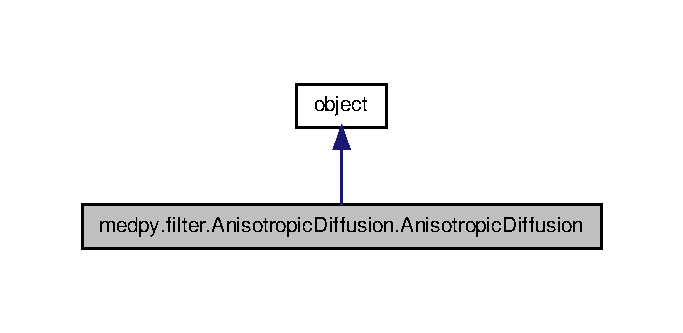
\includegraphics[width=328pt]{classmedpy_1_1filter_1_1AnisotropicDiffusion_1_1AnisotropicDiffusion__inherit__graph}
\end{center}
\end{figure}


Collaboration diagram for medpy.filter.AnisotropicDiffusion.AnisotropicDiffusion:\nopagebreak
\begin{figure}[H]
\begin{center}
\leavevmode
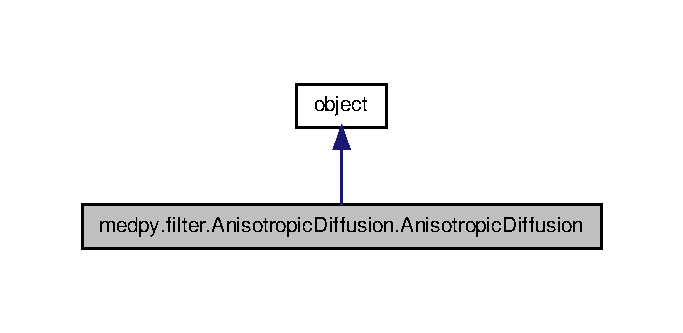
\includegraphics[width=328pt]{classmedpy_1_1filter_1_1AnisotropicDiffusion_1_1AnisotropicDiffusion__coll__graph}
\end{center}
\end{figure}
\subsection*{Public Member Functions}
\begin{DoxyCompactItemize}
\item 
\hypertarget{classmedpy_1_1filter_1_1AnisotropicDiffusion_1_1AnisotropicDiffusion_a44c36411bf89fa4363f8530fd1c95e08}{
def {\bfseries \_\-\_\-init\_\-\_\-}}
\label{classmedpy_1_1filter_1_1AnisotropicDiffusion_1_1AnisotropicDiffusion_a44c36411bf89fa4363f8530fd1c95e08}

\item 
\hypertarget{classmedpy_1_1filter_1_1AnisotropicDiffusion_1_1AnisotropicDiffusion_a0570346712d774d5924136d2db5b1900}{
def {\bfseries anisotropic\_\-diffusion}}
\label{classmedpy_1_1filter_1_1AnisotropicDiffusion_1_1AnisotropicDiffusion_a0570346712d774d5924136d2db5b1900}

\end{DoxyCompactItemize}


\subsection{Detailed Description}


Definition at line 24 of file AnisotropicDiffusion.py.



The documentation for this class was generated from the following file:\begin{DoxyCompactItemize}
\item 
/home/omaier/Programming/Python/medpy/src/medpy/filter/AnisotropicDiffusion.py\end{DoxyCompactItemize}

\hypertarget{classmedpy_1_1core_1_1exceptions_1_1ArgumentError}{
\section{medpy.core.exceptions.ArgumentError Class Reference}
\label{classmedpy_1_1core_1_1exceptions_1_1ArgumentError}\index{medpy::core::exceptions::ArgumentError@{medpy::core::exceptions::ArgumentError}}
}


Thrown by an application when an invalid command line argument has been supplied.  




Inheritance diagram for medpy.core.exceptions.ArgumentError:\nopagebreak
\begin{figure}[H]
\begin{center}
\leavevmode
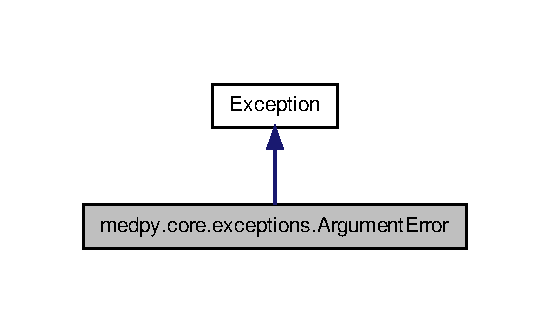
\includegraphics[width=264pt]{classmedpy_1_1core_1_1exceptions_1_1ArgumentError__inherit__graph}
\end{center}
\end{figure}


Collaboration diagram for medpy.core.exceptions.ArgumentError:\nopagebreak
\begin{figure}[H]
\begin{center}
\leavevmode
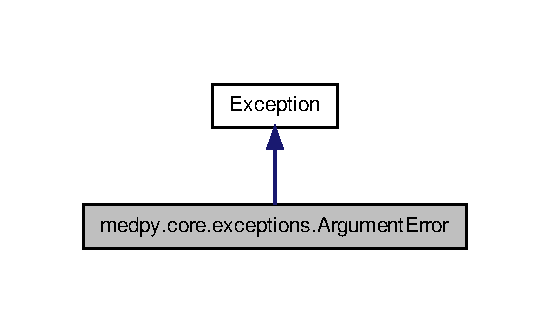
\includegraphics[width=264pt]{classmedpy_1_1core_1_1exceptions_1_1ArgumentError__coll__graph}
\end{center}
\end{figure}


\subsection{Detailed Description}
Thrown by an application when an invalid command line argument has been supplied. 

Definition at line 28 of file exceptions.py.



The documentation for this class was generated from the following file:\begin{DoxyCompactItemize}
\item 
/home/loli/Programming/Python/MedPy/src/medpy/core/exceptions.py\end{DoxyCompactItemize}

\hypertarget{classException}{
\section{Exception Class Reference}
\label{classException}\index{Exception@{Exception}}
}


Inheritance diagram for Exception:\nopagebreak
\begin{figure}[H]
\begin{center}
\leavevmode
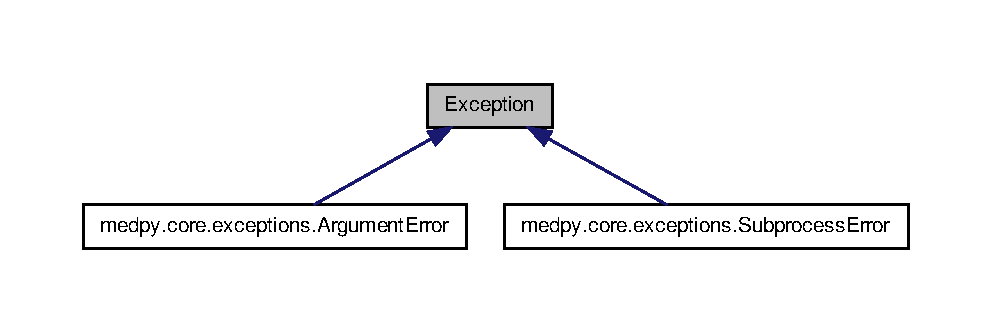
\includegraphics[width=264pt]{classException__inherit__graph}
\end{center}
\end{figure}


The documentation for this class was generated from the following file:\begin{DoxyCompactItemize}
\item 
/home/loli/Programming/Python/MedPy/src/medpy/core/exceptions.py\end{DoxyCompactItemize}

\hypertarget{classmedpy_1_1graphcut_1_1graph_1_1Graph}{
\section{medpy.graphcut.graph.Graph Class Reference}
\label{classmedpy_1_1graphcut_1_1graph_1_1Graph}\index{medpy::graphcut::graph::Graph@{medpy::graphcut::graph::Graph}}
}


Represents a graph suitable for further processing with the graphcut package.  




Inheritance diagram for medpy.graphcut.graph.Graph:\nopagebreak
\begin{figure}[H]
\begin{center}
\leavevmode
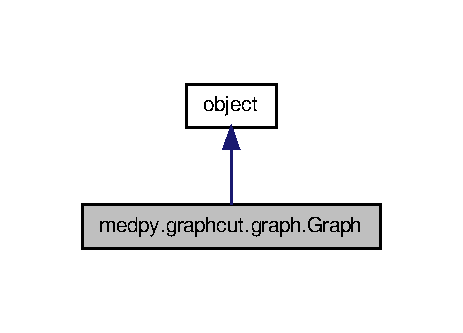
\includegraphics[width=222pt]{classmedpy_1_1graphcut_1_1graph_1_1Graph__inherit__graph}
\end{center}
\end{figure}


Collaboration diagram for medpy.graphcut.graph.Graph:\nopagebreak
\begin{figure}[H]
\begin{center}
\leavevmode
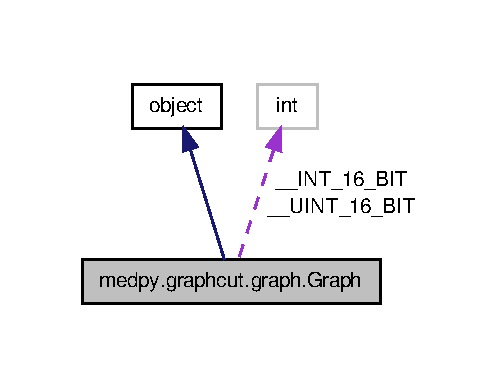
\includegraphics[width=240pt]{classmedpy_1_1graphcut_1_1graph_1_1Graph__coll__graph}
\end{center}
\end{figure}
\subsection*{Public Member Functions}
\begin{DoxyCompactItemize}
\item 
\hypertarget{classmedpy_1_1graphcut_1_1graph_1_1Graph_ada7c2ff7b950159feab5a4d2f69464c9}{
def {\bfseries \_\-\_\-init\_\-\_\-}}
\label{classmedpy_1_1graphcut_1_1graph_1_1Graph_ada7c2ff7b950159feab5a4d2f69464c9}

\item 
def \hyperlink{classmedpy_1_1graphcut_1_1graph_1_1Graph_a41b5d54706b84e5a11523da1ba626848}{set\_\-nodes}
\begin{DoxyCompactList}\small\item\em Set the graphs nodes. \end{DoxyCompactList}\item 
def \hyperlink{classmedpy_1_1graphcut_1_1graph_1_1Graph_af1726ca138ac2522b5fe98f5ae5b157f}{set\_\-source\_\-nodes}
\begin{DoxyCompactList}\small\item\em Set the source nodes and compute their t-\/weights. \end{DoxyCompactList}\item 
def \hyperlink{classmedpy_1_1graphcut_1_1graph_1_1Graph_a54b1a1643e1eedda40c121f9b3e7577d}{set\_\-sink\_\-nodes}
\begin{DoxyCompactList}\small\item\em Set the sink nodes and compute their t-\/weights. \end{DoxyCompactList}\item 
def \hyperlink{classmedpy_1_1graphcut_1_1graph_1_1Graph_a197d5cca5684cebfbabb07f13c4c0175}{set\_\-nweights}
\begin{DoxyCompactList}\small\item\em Sets all nweights. \end{DoxyCompactList}\item 
def \hyperlink{classmedpy_1_1graphcut_1_1graph_1_1Graph_a5a99c76efac37bc31acf495873933122}{add\_\-tweights}
\begin{DoxyCompactList}\small\item\em Adds tweights to the current collection of tweights, overwriting already existing ones. \end{DoxyCompactList}\item 
def \hyperlink{classmedpy_1_1graphcut_1_1graph_1_1Graph_a1cf8f8077a620ae6fd90b327f689d5e5}{get\_\-nodes}
\item 
def \hyperlink{classmedpy_1_1graphcut_1_1graph_1_1Graph_a4c8dbbd92c6b0e5534869890810f0c78}{get\_\-source\_\-nodes}
\item 
def \hyperlink{classmedpy_1_1graphcut_1_1graph_1_1Graph_a988309a34486d834c65d87e83548b969}{get\_\-sink\_\-nodes}
\item 
def \hyperlink{classmedpy_1_1graphcut_1_1graph_1_1Graph_aabbf310726d5af9bbd79c6492f683c11}{get\_\-edges}
\item 
def \hyperlink{classmedpy_1_1graphcut_1_1graph_1_1Graph_a1090dadcdad71f1d629425c917e32ba5}{get\_\-nweights}
\item 
def \hyperlink{classmedpy_1_1graphcut_1_1graph_1_1Graph_a4b033a8067128c8a222f6c466f1b606f}{get\_\-tweights}
\item 
def \hyperlink{classmedpy_1_1graphcut_1_1graph_1_1Graph_a0441ff798c06ebf4cb860af7ccf37a36}{get\_\-tweights2}
\begin{DoxyCompactList}\small\item\em Version of  \hyperlink{classmedpy_1_1graphcut_1_1graph_1_1Graph_a4b033a8067128c8a222f6c466f1b606f}{get\_\-tweights()} that does not check if all tweights has been set and is therefore slightly faster. \end{DoxyCompactList}\item 
def \hyperlink{classmedpy_1_1graphcut_1_1graph_1_1Graph_a0fbe2b59f746e726f8bcf6c3111d7860}{inconsistent}
\begin{DoxyCompactList}\small\item\em Perform some consistency tests on the graph represented by this object. \end{DoxyCompactList}\end{DoxyCompactItemize}
\subsection*{Static Public Attributes}
\begin{DoxyCompactItemize}
\item 
\hypertarget{classmedpy_1_1graphcut_1_1graph_1_1Graph_aaed442199a4e04230982c1eb5cf809df}{
{\bfseries MAX} = \_\-\_\-UINT\_\-16\_\-BIT}
\label{classmedpy_1_1graphcut_1_1graph_1_1Graph_aaed442199a4e04230982c1eb5cf809df}

\end{DoxyCompactItemize}


\subsection{Detailed Description}
Represents a graph suitable for further processing with the graphcut package. 

The graph contains nodes, edges (directed) between the nodes (n-\/edges), edges between two terminals (called source and sink) and the edges (t-\/edges) and a weight for each edge.

Methods: set\_\-nodes(nodes) -\/-\/ Set the nodes. set\_\-source\_\-nodes(source\_\-nodes) -\/-\/ Set the source nodes. set\_\-sink\_\-nodes(sink\_\-nodes) -\/-\/ Set the sink nodes. set\_\-nweights(nweights) -\/-\/ Set the inter-\/node weights-\/ add\_\-tweights(nweights) -\/-\/ Add some terminal-\/to-\/node weights. \hyperlink{classmedpy_1_1graphcut_1_1graph_1_1Graph_a1cf8f8077a620ae6fd90b327f689d5e5}{get\_\-nodes()} -\/-\/ Return all nodes. \hyperlink{classmedpy_1_1graphcut_1_1graph_1_1Graph_a4c8dbbd92c6b0e5534869890810f0c78}{get\_\-source\_\-nodes()} -\/-\/ Return all nodes connected to the source. \hyperlink{classmedpy_1_1graphcut_1_1graph_1_1Graph_a988309a34486d834c65d87e83548b969}{get\_\-sink\_\-nodes()} -\/-\/ Return all nodes connected to the sink. \hyperlink{classmedpy_1_1graphcut_1_1graph_1_1Graph_aabbf310726d5af9bbd79c6492f683c11}{get\_\-edges()} -\/-\/ Return all edges. \hyperlink{classmedpy_1_1graphcut_1_1graph_1_1Graph_a1090dadcdad71f1d629425c917e32ba5}{get\_\-nweights()} -\/-\/ Return all inter-\/node weights. \hyperlink{classmedpy_1_1graphcut_1_1graph_1_1Graph_a4b033a8067128c8a222f6c466f1b606f}{get\_\-tweights()} -\/-\/ Return all terminal-\/node weights. \hyperlink{classmedpy_1_1graphcut_1_1graph_1_1Graph_a0441ff798c06ebf4cb860af7ccf37a36}{get\_\-tweights2()} -\/-\/ Unsave version of \hyperlink{classmedpy_1_1graphcut_1_1graph_1_1Graph_a4b033a8067128c8a222f6c466f1b606f}{get\_\-tweights()} 

Definition at line 62 of file graph.py.



\subsection{Member Function Documentation}
\hypertarget{classmedpy_1_1graphcut_1_1graph_1_1Graph_a5a99c76efac37bc31acf495873933122}{
\index{medpy::graphcut::graph::Graph@{medpy::graphcut::graph::Graph}!add\_\-tweights@{add\_\-tweights}}
\index{add\_\-tweights@{add\_\-tweights}!medpy::graphcut::graph::Graph@{medpy::graphcut::graph::Graph}}
\subsubsection[{add\_\-tweights}]{\setlength{\rightskip}{0pt plus 5cm}def medpy.graphcut.graph.Graph.add\_\-tweights (
\begin{DoxyParamCaption}
\item[{}]{self, }
\item[{}]{tweights}
\end{DoxyParamCaption}
)}}
\label{classmedpy_1_1graphcut_1_1graph_1_1Graph_a5a99c76efac37bc31acf495873933122}


Adds tweights to the current collection of tweights, overwriting already existing ones. 


\begin{DoxyParams}{Parameters}
{\em tweights,:} & a dictionary with node\_\-ids as keys and (weight-\/to-\/soource, weight-\/to-\/sink) tuples as values.  tweights: dict \\
\hline
\end{DoxyParams}


Definition at line 145 of file graph.py.

\hypertarget{classmedpy_1_1graphcut_1_1graph_1_1Graph_aabbf310726d5af9bbd79c6492f683c11}{
\index{medpy::graphcut::graph::Graph@{medpy::graphcut::graph::Graph}!get\_\-edges@{get\_\-edges}}
\index{get\_\-edges@{get\_\-edges}!medpy::graphcut::graph::Graph@{medpy::graphcut::graph::Graph}}
\subsubsection[{get\_\-edges}]{\setlength{\rightskip}{0pt plus 5cm}def medpy.graphcut.graph.Graph.get\_\-edges (
\begin{DoxyParamCaption}
\item[{}]{self}
\end{DoxyParamCaption}
)}}
\label{classmedpy_1_1graphcut_1_1graph_1_1Graph_aabbf310726d5af9bbd79c6492f683c11}
\begin{DoxyReturn}{Returns}
: all edges as ordered list of tuples (i.e. \mbox{[}(node\_\-id1, node\_\-id2), (..), ...\mbox{]}. : list 
\end{DoxyReturn}


Definition at line 177 of file graph.py.

\hypertarget{classmedpy_1_1graphcut_1_1graph_1_1Graph_a1cf8f8077a620ae6fd90b327f689d5e5}{
\index{medpy::graphcut::graph::Graph@{medpy::graphcut::graph::Graph}!get\_\-nodes@{get\_\-nodes}}
\index{get\_\-nodes@{get\_\-nodes}!medpy::graphcut::graph::Graph@{medpy::graphcut::graph::Graph}}
\subsubsection[{get\_\-nodes}]{\setlength{\rightskip}{0pt plus 5cm}def medpy.graphcut.graph.Graph.get\_\-nodes (
\begin{DoxyParamCaption}
\item[{}]{self}
\end{DoxyParamCaption}
)}}
\label{classmedpy_1_1graphcut_1_1graph_1_1Graph_a1cf8f8077a620ae6fd90b327f689d5e5}
\begin{DoxyReturn}{Returns}
all nodes as an unordered list. : list 
\end{DoxyReturn}


Definition at line 153 of file graph.py.

\hypertarget{classmedpy_1_1graphcut_1_1graph_1_1Graph_a1090dadcdad71f1d629425c917e32ba5}{
\index{medpy::graphcut::graph::Graph@{medpy::graphcut::graph::Graph}!get\_\-nweights@{get\_\-nweights}}
\index{get\_\-nweights@{get\_\-nweights}!medpy::graphcut::graph::Graph@{medpy::graphcut::graph::Graph}}
\subsubsection[{get\_\-nweights}]{\setlength{\rightskip}{0pt plus 5cm}def medpy.graphcut.graph.Graph.get\_\-nweights (
\begin{DoxyParamCaption}
\item[{}]{self}
\end{DoxyParamCaption}
)}}
\label{classmedpy_1_1graphcut_1_1graph_1_1Graph_a1090dadcdad71f1d629425c917e32ba5}
\begin{DoxyReturn}{Returns}
: all n-\/weights (inter-\/node weights) as \{edge-\/tuple: weight, ...\} dict. : dict 
\end{DoxyReturn}


Definition at line 185 of file graph.py.

\hypertarget{classmedpy_1_1graphcut_1_1graph_1_1Graph_a988309a34486d834c65d87e83548b969}{
\index{medpy::graphcut::graph::Graph@{medpy::graphcut::graph::Graph}!get\_\-sink\_\-nodes@{get\_\-sink\_\-nodes}}
\index{get\_\-sink\_\-nodes@{get\_\-sink\_\-nodes}!medpy::graphcut::graph::Graph@{medpy::graphcut::graph::Graph}}
\subsubsection[{get\_\-sink\_\-nodes}]{\setlength{\rightskip}{0pt plus 5cm}def medpy.graphcut.graph.Graph.get\_\-sink\_\-nodes (
\begin{DoxyParamCaption}
\item[{}]{self}
\end{DoxyParamCaption}
)}}
\label{classmedpy_1_1graphcut_1_1graph_1_1Graph_a988309a34486d834c65d87e83548b969}
\begin{DoxyReturn}{Returns}
: all nodes that are connected with the source as an unordered list. : list 
\end{DoxyReturn}


Definition at line 169 of file graph.py.

\hypertarget{classmedpy_1_1graphcut_1_1graph_1_1Graph_a4c8dbbd92c6b0e5534869890810f0c78}{
\index{medpy::graphcut::graph::Graph@{medpy::graphcut::graph::Graph}!get\_\-source\_\-nodes@{get\_\-source\_\-nodes}}
\index{get\_\-source\_\-nodes@{get\_\-source\_\-nodes}!medpy::graphcut::graph::Graph@{medpy::graphcut::graph::Graph}}
\subsubsection[{get\_\-source\_\-nodes}]{\setlength{\rightskip}{0pt plus 5cm}def medpy.graphcut.graph.Graph.get\_\-source\_\-nodes (
\begin{DoxyParamCaption}
\item[{}]{self}
\end{DoxyParamCaption}
)}}
\label{classmedpy_1_1graphcut_1_1graph_1_1Graph_a4c8dbbd92c6b0e5534869890810f0c78}
\begin{DoxyReturn}{Returns}
: all nodes that are connected with the source as an unordered list. : list 
\end{DoxyReturn}


Definition at line 161 of file graph.py.

\hypertarget{classmedpy_1_1graphcut_1_1graph_1_1Graph_a4b033a8067128c8a222f6c466f1b606f}{
\index{medpy::graphcut::graph::Graph@{medpy::graphcut::graph::Graph}!get\_\-tweights@{get\_\-tweights}}
\index{get\_\-tweights@{get\_\-tweights}!medpy::graphcut::graph::Graph@{medpy::graphcut::graph::Graph}}
\subsubsection[{get\_\-tweights}]{\setlength{\rightskip}{0pt plus 5cm}def medpy.graphcut.graph.Graph.get\_\-tweights (
\begin{DoxyParamCaption}
\item[{}]{self}
\end{DoxyParamCaption}
)}}
\label{classmedpy_1_1graphcut_1_1graph_1_1Graph_a4b033a8067128c8a222f6c466f1b606f}
\begin{DoxyReturn}{Returns}
: all t-\/weights (terminal-\/node weights) as \{node\_\-id: weight, ...\} dict. : dict 
\end{DoxyReturn}


Definition at line 193 of file graph.py.

\hypertarget{classmedpy_1_1graphcut_1_1graph_1_1Graph_a0441ff798c06ebf4cb860af7ccf37a36}{
\index{medpy::graphcut::graph::Graph@{medpy::graphcut::graph::Graph}!get\_\-tweights2@{get\_\-tweights2}}
\index{get\_\-tweights2@{get\_\-tweights2}!medpy::graphcut::graph::Graph@{medpy::graphcut::graph::Graph}}
\subsubsection[{get\_\-tweights2}]{\setlength{\rightskip}{0pt plus 5cm}def medpy.graphcut.graph.Graph.get\_\-tweights2 (
\begin{DoxyParamCaption}
\item[{}]{self}
\end{DoxyParamCaption}
)}}
\label{classmedpy_1_1graphcut_1_1graph_1_1Graph_a0441ff798c06ebf4cb860af7ccf37a36}


Version of  \hyperlink{classmedpy_1_1graphcut_1_1graph_1_1Graph_a4b033a8067128c8a222f6c466f1b606f}{get\_\-tweights()} that does not check if all tweights has been set and is therefore slightly faster. 

Use with caution! \begin{DoxyReturn}{Returns}
: all t-\/weights (terminal-\/node weights) as \{node\_\-id: weight, ...\} dict. : dict 
\end{DoxyReturn}


Definition at line 208 of file graph.py.

\hypertarget{classmedpy_1_1graphcut_1_1graph_1_1Graph_a0fbe2b59f746e726f8bcf6c3111d7860}{
\index{medpy::graphcut::graph::Graph@{medpy::graphcut::graph::Graph}!inconsistent@{inconsistent}}
\index{inconsistent@{inconsistent}!medpy::graphcut::graph::Graph@{medpy::graphcut::graph::Graph}}
\subsubsection[{inconsistent}]{\setlength{\rightskip}{0pt plus 5cm}def medpy.graphcut.graph.Graph.inconsistent (
\begin{DoxyParamCaption}
\item[{}]{self}
\end{DoxyParamCaption}
)}}
\label{classmedpy_1_1graphcut_1_1graph_1_1Graph_a0fbe2b59f746e726f8bcf6c3111d7860}


Perform some consistency tests on the graph represented by this object. 

\begin{DoxyReturn}{Returns}
: False if consistent, else a list of inconsistency messages. 
\end{DoxyReturn}


Definition at line 216 of file graph.py.

\hypertarget{classmedpy_1_1graphcut_1_1graph_1_1Graph_a41b5d54706b84e5a11523da1ba626848}{
\index{medpy::graphcut::graph::Graph@{medpy::graphcut::graph::Graph}!set\_\-nodes@{set\_\-nodes}}
\index{set\_\-nodes@{set\_\-nodes}!medpy::graphcut::graph::Graph@{medpy::graphcut::graph::Graph}}
\subsubsection[{set\_\-nodes}]{\setlength{\rightskip}{0pt plus 5cm}def medpy.graphcut.graph.Graph.set\_\-nodes (
\begin{DoxyParamCaption}
\item[{}]{self, }
\item[{}]{nodes}
\end{DoxyParamCaption}
)}}
\label{classmedpy_1_1graphcut_1_1graph_1_1Graph_a41b5d54706b84e5a11523da1ba626848}


Set the graphs nodes. 


\begin{DoxyParams}{Parameters}
{\em nodes,:} & a sequence of integers  nodes: sequence \\
\hline
\end{DoxyParams}


Definition at line 85 of file graph.py.

\hypertarget{classmedpy_1_1graphcut_1_1graph_1_1Graph_a197d5cca5684cebfbabb07f13c4c0175}{
\index{medpy::graphcut::graph::Graph@{medpy::graphcut::graph::Graph}!set\_\-nweights@{set\_\-nweights}}
\index{set\_\-nweights@{set\_\-nweights}!medpy::graphcut::graph::Graph@{medpy::graphcut::graph::Graph}}
\subsubsection[{set\_\-nweights}]{\setlength{\rightskip}{0pt plus 5cm}def medpy.graphcut.graph.Graph.set\_\-nweights (
\begin{DoxyParamCaption}
\item[{}]{self, }
\item[{}]{nweights}
\end{DoxyParamCaption}
)}}
\label{classmedpy_1_1graphcut_1_1graph_1_1Graph_a197d5cca5684cebfbabb07f13c4c0175}


Sets all nweights. 


\begin{DoxyParams}{Parameters}
{\em nweights,:} & a dictionary with (region-\/a-\/id, region-\/b-\/id) tuples as keys and (weight-\/a-\/to-\/b, weight-\/b-\/to-\/a) as values.  nweights: dict \\
\hline
\end{DoxyParams}


Definition at line 135 of file graph.py.

\hypertarget{classmedpy_1_1graphcut_1_1graph_1_1Graph_a54b1a1643e1eedda40c121f9b3e7577d}{
\index{medpy::graphcut::graph::Graph@{medpy::graphcut::graph::Graph}!set\_\-sink\_\-nodes@{set\_\-sink\_\-nodes}}
\index{set\_\-sink\_\-nodes@{set\_\-sink\_\-nodes}!medpy::graphcut::graph::Graph@{medpy::graphcut::graph::Graph}}
\subsubsection[{set\_\-sink\_\-nodes}]{\setlength{\rightskip}{0pt plus 5cm}def medpy.graphcut.graph.Graph.set\_\-sink\_\-nodes (
\begin{DoxyParamCaption}
\item[{}]{self, }
\item[{}]{sink\_\-nodes}
\end{DoxyParamCaption}
)}}
\label{classmedpy_1_1graphcut_1_1graph_1_1Graph_a54b1a1643e1eedda40c121f9b3e7577d}


Set the sink nodes and compute their t-\/weights. 

\begin{DoxyWarning}{Warning}
: It does not get checked if one of the supplied sink-\/nodes already has a weight assigned (e.g. by passing it to  \hyperlink{classmedpy_1_1graphcut_1_1graph_1_1Graph_af1726ca138ac2522b5fe98f5ae5b157f}{set\_\-source\_\-nodes()}). This can occur when the foreground-\/ and background-\/markers cover the same region. In this case the order of setting the terminal nodes can affect the graph and therefore the graph-\/cut result.
\end{DoxyWarning}

\begin{DoxyParams}{Parameters}
{\em sink\_\-nodes,:} & a sequence of integers  sink\_\-nodes: sequence \\
\hline
\end{DoxyParams}


Definition at line 121 of file graph.py.

\hypertarget{classmedpy_1_1graphcut_1_1graph_1_1Graph_af1726ca138ac2522b5fe98f5ae5b157f}{
\index{medpy::graphcut::graph::Graph@{medpy::graphcut::graph::Graph}!set\_\-source\_\-nodes@{set\_\-source\_\-nodes}}
\index{set\_\-source\_\-nodes@{set\_\-source\_\-nodes}!medpy::graphcut::graph::Graph@{medpy::graphcut::graph::Graph}}
\subsubsection[{set\_\-source\_\-nodes}]{\setlength{\rightskip}{0pt plus 5cm}def medpy.graphcut.graph.Graph.set\_\-source\_\-nodes (
\begin{DoxyParamCaption}
\item[{}]{self, }
\item[{}]{source\_\-nodes}
\end{DoxyParamCaption}
)}}
\label{classmedpy_1_1graphcut_1_1graph_1_1Graph_af1726ca138ac2522b5fe98f5ae5b157f}


Set the source nodes and compute their t-\/weights. 

\begin{DoxyWarning}{Warning}
: It does not get checked if one of the supplied source-\/nodes already has a weight assigned (e.g. by passing it to  \hyperlink{classmedpy_1_1graphcut_1_1graph_1_1Graph_a54b1a1643e1eedda40c121f9b3e7577d}{set\_\-sink\_\-nodes()}). This can occur when the foreground-\/ and background-\/markers cover the same region. In this case the order of setting the terminal nodes can affect the graph and therefore the graph-\/cut result.
\end{DoxyWarning}

\begin{DoxyParams}{Parameters}
{\em source\_\-nodes,:} & a sequence of integers  source\_\-nodes: sequence \\
\hline
\end{DoxyParams}


Definition at line 101 of file graph.py.



The documentation for this class was generated from the following file:\begin{DoxyCompactItemize}
\item 
/home/omaier/Programming/Python/medpy/src/medpy/graphcut/graph.py\end{DoxyCompactItemize}

\hypertarget{classmedpy_1_1filter_1_1LabelImageStatistics_1_1LabelImageStatistics}{
\section{medpy.filter.LabelImageStatistics.LabelImageStatistics Class Reference}
\label{classmedpy_1_1filter_1_1LabelImageStatistics_1_1LabelImageStatistics}\index{medpy::filter::LabelImageStatistics::LabelImageStatistics@{medpy::filter::LabelImageStatistics::LabelImageStatistics}}
}


Collaboration diagram for medpy.filter.LabelImageStatistics.LabelImageStatistics:\nopagebreak
\begin{figure}[H]
\begin{center}
\leavevmode
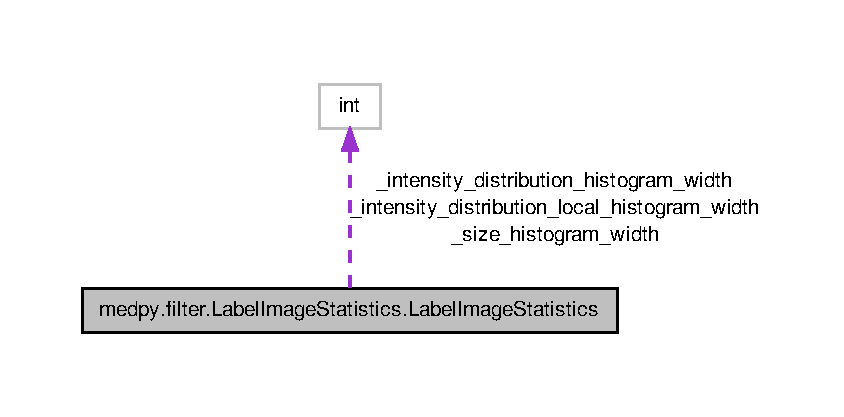
\includegraphics[width=400pt]{classmedpy_1_1filter_1_1LabelImageStatistics_1_1LabelImageStatistics__coll__graph}
\end{center}
\end{figure}
\subsection*{Public Member Functions}
\begin{DoxyCompactItemize}
\item 
def \hyperlink{classmedpy_1_1filter_1_1LabelImageStatistics_1_1LabelImageStatistics_a930a01ac2051dbe15724f1e15190a490}{\_\-\_\-init\_\-\_\-}
\begin{DoxyCompactList}\small\item\em Computes a number of statistics for the labels of a label image. \end{DoxyCompactList}\item 
def \hyperlink{classmedpy_1_1filter_1_1LabelImageStatistics_1_1LabelImageStatistics_aa4b41c43fb9700962e483b6f450b4710}{get\_\-size\_\-histogram\_\-width}
\item 
def \hyperlink{classmedpy_1_1filter_1_1LabelImageStatistics_1_1LabelImageStatistics_a13532e9b0424fca8258bde4f6f4f1a6a}{get\_\-intensity\_\-distribution\_\-histogram\_\-width}
\item 
def \hyperlink{classmedpy_1_1filter_1_1LabelImageStatistics_1_1LabelImageStatistics_af9ec002c180c90a40ca414727145103d}{set\_\-size\_\-histogram\_\-width}
\begin{DoxyCompactList}\small\item\em Set the width and therefore granularity of. \end{DoxyCompactList}\item 
def \hyperlink{classmedpy_1_1filter_1_1LabelImageStatistics_1_1LabelImageStatistics_aa0c7b77ccddc07ab789eb1d5bb5cbc5f}{set\_\-intensity\_\-distribution\_\-histogram\_\-width}
\begin{DoxyCompactList}\small\item\em Set the width and therefore granularity of. \end{DoxyCompactList}\item 
def \hyperlink{classmedpy_1_1filter_1_1LabelImageStatistics_1_1LabelImageStatistics_a157a8d51427bf37302ca4a06c1aedb65}{labels\_\-are\_\-consecutive}
\item 
def \hyperlink{classmedpy_1_1filter_1_1LabelImageStatistics_1_1LabelImageStatistics_aa2f28c8938d0c378f4c61eff849bf9fb}{get\_\-min\_\-intensity}
\item 
def \hyperlink{classmedpy_1_1filter_1_1LabelImageStatistics_1_1LabelImageStatistics_afa86e54a37287134a82f44caf14e995a}{get\_\-max\_\-intensity}
\item 
def \hyperlink{classmedpy_1_1filter_1_1LabelImageStatistics_1_1LabelImageStatistics_a257d8c1a5996612b6e38257316c8eb4d}{get\_\-min\_\-label}
\item 
def \hyperlink{classmedpy_1_1filter_1_1LabelImageStatistics_1_1LabelImageStatistics_a178846f8509e6dc284f1280827720a36}{get\_\-max\_\-label}
\item 
def \hyperlink{classmedpy_1_1filter_1_1LabelImageStatistics_1_1LabelImageStatistics_a4a4efd07eeb97f0474d6b0938f1c9346}{get\_\-label\_\-count}
\item 
def \hyperlink{classmedpy_1_1filter_1_1LabelImageStatistics_1_1LabelImageStatistics_a22329b52becafadd81103650e5bd0da1}{get\_\-sizes}
\item 
def \hyperlink{classmedpy_1_1filter_1_1LabelImageStatistics_1_1LabelImageStatistics_a418bb33624949145cdc0fe1fa6562451}{get\_\-size\_\-histogram}
\begin{DoxyCompactList}\small\item\em Gives the region size distribution. \end{DoxyCompactList}\item 
def \hyperlink{classmedpy_1_1filter_1_1LabelImageStatistics_1_1LabelImageStatistics_a9bea3a398baf6ee92218fc257474ee4a}{get\_\-intensity\_\-distributions}
\item 
def \hyperlink{classmedpy_1_1filter_1_1LabelImageStatistics_1_1LabelImageStatistics_a37da9517c63c76675a4df75c2d13d672}{get\_\-intensity\_\-distribution\_\-histogram}
\begin{DoxyCompactList}\small\item\em Gives the distribution of the smoothness of the intensity distribution in each region. \end{DoxyCompactList}\end{DoxyCompactItemize}


\subsection{Detailed Description}
\begin{DoxyVerb}The label image.\end{DoxyVerb}
 

Definition at line 25 of file LabelImageStatistics.py.



\subsection{Constructor \& Destructor Documentation}
\hypertarget{classmedpy_1_1filter_1_1LabelImageStatistics_1_1LabelImageStatistics_a930a01ac2051dbe15724f1e15190a490}{
\index{medpy::filter::LabelImageStatistics::LabelImageStatistics@{medpy::filter::LabelImageStatistics::LabelImageStatistics}!\_\-\_\-init\_\-\_\-@{\_\-\_\-init\_\-\_\-}}
\index{\_\-\_\-init\_\-\_\-@{\_\-\_\-init\_\-\_\-}!medpy::filter::LabelImageStatistics::LabelImageStatistics@{medpy::filter::LabelImageStatistics::LabelImageStatistics}}
\subsubsection[{\_\-\_\-init\_\-\_\-}]{\setlength{\rightskip}{0pt plus 5cm}def medpy.filter.LabelImageStatistics.LabelImageStatistics.\_\-\_\-init\_\-\_\- (
\begin{DoxyParamCaption}
\item[{}]{self, }
\item[{}]{image\_\-labels, }
\item[{}]{image\_\-original}
\end{DoxyParamCaption}
)}}
\label{classmedpy_1_1filter_1_1LabelImageStatistics_1_1LabelImageStatistics_a930a01ac2051dbe15724f1e15190a490}


Computes a number of statistics for the labels of a label image. 

These include beside others: 1. a histogram of the sizes of the regions 2. a histogram of the sphericity (not roundness) of the regions 3. a histogram of how the intensity distribution in each region differs from a Gaussian distribution


\begin{DoxyParams}{Parameters}
{\em image\_\-lables,:} & The label image for which the statistics should be computed as a numpy array \\
\hline
{\em image\_\-original,:} & The original image for which the label image was created. \\
\hline
\end{DoxyParams}


Definition at line 55 of file LabelImageStatistics.py.



\subsection{Member Function Documentation}
\hypertarget{classmedpy_1_1filter_1_1LabelImageStatistics_1_1LabelImageStatistics_a37da9517c63c76675a4df75c2d13d672}{
\index{medpy::filter::LabelImageStatistics::LabelImageStatistics@{medpy::filter::LabelImageStatistics::LabelImageStatistics}!get\_\-intensity\_\-distribution\_\-histogram@{get\_\-intensity\_\-distribution\_\-histogram}}
\index{get\_\-intensity\_\-distribution\_\-histogram@{get\_\-intensity\_\-distribution\_\-histogram}!medpy::filter::LabelImageStatistics::LabelImageStatistics@{medpy::filter::LabelImageStatistics::LabelImageStatistics}}
\subsubsection[{get\_\-intensity\_\-distribution\_\-histogram}]{\setlength{\rightskip}{0pt plus 5cm}def medpy.filter.LabelImageStatistics.LabelImageStatistics.get\_\-intensity\_\-distribution\_\-histogram (
\begin{DoxyParamCaption}
\item[{}]{self}
\end{DoxyParamCaption}
)}}
\label{classmedpy_1_1filter_1_1LabelImageStatistics_1_1LabelImageStatistics_a37da9517c63c76675a4df75c2d13d672}


Gives the distribution of the smoothness of the intensity distribution in each region. 

\begin{DoxyReturn}{Returns}
: A histogram created from the normalized distances between each regions intensity distribution and a ideally fitted Gaussian with scipy.histogram.
\end{DoxyReturn}
The raw values can be extracted using \begin{DoxySeeAlso}{See also}
: \hyperlink{classmedpy_1_1filter_1_1LabelImageStatistics_1_1LabelImageStatistics_a9bea3a398baf6ee92218fc257474ee4a}{LabelImageStatistics.get\_\-intensity\_\-distributions}.
\end{DoxySeeAlso}
\begin{DoxyNote}{Note}
: The width and therefore the number of distinct values of the histogram can be set with 
\end{DoxyNote}
\begin{DoxySeeAlso}{See also}
: \hyperlink{classmedpy_1_1filter_1_1LabelImageStatistics_1_1LabelImageStatistics_aa0c7b77ccddc07ab789eb1d5bb5cbc5f}{LabelImageStatistics.set\_\-intensity\_\-distribution\_\-histogram\_\-width}. 
\end{DoxySeeAlso}


Definition at line 189 of file LabelImageStatistics.py.

\hypertarget{classmedpy_1_1filter_1_1LabelImageStatistics_1_1LabelImageStatistics_a13532e9b0424fca8258bde4f6f4f1a6a}{
\index{medpy::filter::LabelImageStatistics::LabelImageStatistics@{medpy::filter::LabelImageStatistics::LabelImageStatistics}!get\_\-intensity\_\-distribution\_\-histogram\_\-width@{get\_\-intensity\_\-distribution\_\-histogram\_\-width}}
\index{get\_\-intensity\_\-distribution\_\-histogram\_\-width@{get\_\-intensity\_\-distribution\_\-histogram\_\-width}!medpy::filter::LabelImageStatistics::LabelImageStatistics@{medpy::filter::LabelImageStatistics::LabelImageStatistics}}
\subsubsection[{get\_\-intensity\_\-distribution\_\-histogram\_\-width}]{\setlength{\rightskip}{0pt plus 5cm}def medpy.filter.LabelImageStatistics.LabelImageStatistics.get\_\-intensity\_\-distribution\_\-histogram\_\-width (
\begin{DoxyParamCaption}
\item[{}]{self}
\end{DoxyParamCaption}
)}}
\label{classmedpy_1_1filter_1_1LabelImageStatistics_1_1LabelImageStatistics_a13532e9b0424fca8258bde4f6f4f1a6a}
\begin{DoxySeeAlso}{See also}
: \hyperlink{classmedpy_1_1filter_1_1LabelImageStatistics_1_1LabelImageStatistics_aa0c7b77ccddc07ab789eb1d5bb5cbc5f}{set\_\-intensity\_\-distribution\_\-histogram\_\-width} 
\end{DoxySeeAlso}


Definition at line 82 of file LabelImageStatistics.py.

\hypertarget{classmedpy_1_1filter_1_1LabelImageStatistics_1_1LabelImageStatistics_a9bea3a398baf6ee92218fc257474ee4a}{
\index{medpy::filter::LabelImageStatistics::LabelImageStatistics@{medpy::filter::LabelImageStatistics::LabelImageStatistics}!get\_\-intensity\_\-distributions@{get\_\-intensity\_\-distributions}}
\index{get\_\-intensity\_\-distributions@{get\_\-intensity\_\-distributions}!medpy::filter::LabelImageStatistics::LabelImageStatistics@{medpy::filter::LabelImageStatistics::LabelImageStatistics}}
\subsubsection[{get\_\-intensity\_\-distributions}]{\setlength{\rightskip}{0pt plus 5cm}def medpy.filter.LabelImageStatistics.LabelImageStatistics.get\_\-intensity\_\-distributions (
\begin{DoxyParamCaption}
\item[{}]{self}
\end{DoxyParamCaption}
)}}
\label{classmedpy_1_1filter_1_1LabelImageStatistics_1_1LabelImageStatistics_a9bea3a398baf6ee92218fc257474ee4a}
\begin{DoxyReturn}{Returns}
: A dictionary with the labels as keys and the convolution of their intensity distribution from an ideal Gaussian as values. 
\end{DoxyReturn}


Definition at line 174 of file LabelImageStatistics.py.

\hypertarget{classmedpy_1_1filter_1_1LabelImageStatistics_1_1LabelImageStatistics_a4a4efd07eeb97f0474d6b0938f1c9346}{
\index{medpy::filter::LabelImageStatistics::LabelImageStatistics@{medpy::filter::LabelImageStatistics::LabelImageStatistics}!get\_\-label\_\-count@{get\_\-label\_\-count}}
\index{get\_\-label\_\-count@{get\_\-label\_\-count}!medpy::filter::LabelImageStatistics::LabelImageStatistics@{medpy::filter::LabelImageStatistics::LabelImageStatistics}}
\subsubsection[{get\_\-label\_\-count}]{\setlength{\rightskip}{0pt plus 5cm}def medpy.filter.LabelImageStatistics.LabelImageStatistics.get\_\-label\_\-count (
\begin{DoxyParamCaption}
\item[{}]{self}
\end{DoxyParamCaption}
)}}
\label{classmedpy_1_1filter_1_1LabelImageStatistics_1_1LabelImageStatistics_a4a4efd07eeb97f0474d6b0938f1c9346}
\begin{DoxyReturn}{Returns}
: The number of labels in the label image 
\end{DoxyReturn}


Definition at line 147 of file LabelImageStatistics.py.

\hypertarget{classmedpy_1_1filter_1_1LabelImageStatistics_1_1LabelImageStatistics_afa86e54a37287134a82f44caf14e995a}{
\index{medpy::filter::LabelImageStatistics::LabelImageStatistics@{medpy::filter::LabelImageStatistics::LabelImageStatistics}!get\_\-max\_\-intensity@{get\_\-max\_\-intensity}}
\index{get\_\-max\_\-intensity@{get\_\-max\_\-intensity}!medpy::filter::LabelImageStatistics::LabelImageStatistics@{medpy::filter::LabelImageStatistics::LabelImageStatistics}}
\subsubsection[{get\_\-max\_\-intensity}]{\setlength{\rightskip}{0pt plus 5cm}def medpy.filter.LabelImageStatistics.LabelImageStatistics.get\_\-max\_\-intensity (
\begin{DoxyParamCaption}
\item[{}]{self}
\end{DoxyParamCaption}
)}}
\label{classmedpy_1_1filter_1_1LabelImageStatistics_1_1LabelImageStatistics_afa86e54a37287134a82f44caf14e995a}
\begin{DoxyReturn}{Returns}
: the original images maximum intensity 
\end{DoxyReturn}


Definition at line 126 of file LabelImageStatistics.py.

\hypertarget{classmedpy_1_1filter_1_1LabelImageStatistics_1_1LabelImageStatistics_a178846f8509e6dc284f1280827720a36}{
\index{medpy::filter::LabelImageStatistics::LabelImageStatistics@{medpy::filter::LabelImageStatistics::LabelImageStatistics}!get\_\-max\_\-label@{get\_\-max\_\-label}}
\index{get\_\-max\_\-label@{get\_\-max\_\-label}!medpy::filter::LabelImageStatistics::LabelImageStatistics@{medpy::filter::LabelImageStatistics::LabelImageStatistics}}
\subsubsection[{get\_\-max\_\-label}]{\setlength{\rightskip}{0pt plus 5cm}def medpy.filter.LabelImageStatistics.LabelImageStatistics.get\_\-max\_\-label (
\begin{DoxyParamCaption}
\item[{}]{self}
\end{DoxyParamCaption}
)}}
\label{classmedpy_1_1filter_1_1LabelImageStatistics_1_1LabelImageStatistics_a178846f8509e6dc284f1280827720a36}
\begin{DoxyReturn}{Returns}
: the largest label index in the label image 
\end{DoxyReturn}


Definition at line 140 of file LabelImageStatistics.py.

\hypertarget{classmedpy_1_1filter_1_1LabelImageStatistics_1_1LabelImageStatistics_aa2f28c8938d0c378f4c61eff849bf9fb}{
\index{medpy::filter::LabelImageStatistics::LabelImageStatistics@{medpy::filter::LabelImageStatistics::LabelImageStatistics}!get\_\-min\_\-intensity@{get\_\-min\_\-intensity}}
\index{get\_\-min\_\-intensity@{get\_\-min\_\-intensity}!medpy::filter::LabelImageStatistics::LabelImageStatistics@{medpy::filter::LabelImageStatistics::LabelImageStatistics}}
\subsubsection[{get\_\-min\_\-intensity}]{\setlength{\rightskip}{0pt plus 5cm}def medpy.filter.LabelImageStatistics.LabelImageStatistics.get\_\-min\_\-intensity (
\begin{DoxyParamCaption}
\item[{}]{self}
\end{DoxyParamCaption}
)}}
\label{classmedpy_1_1filter_1_1LabelImageStatistics_1_1LabelImageStatistics_aa2f28c8938d0c378f4c61eff849bf9fb}
\begin{DoxyReturn}{Returns}
: the original images minimium intensity 
\end{DoxyReturn}


Definition at line 119 of file LabelImageStatistics.py.

\hypertarget{classmedpy_1_1filter_1_1LabelImageStatistics_1_1LabelImageStatistics_a257d8c1a5996612b6e38257316c8eb4d}{
\index{medpy::filter::LabelImageStatistics::LabelImageStatistics@{medpy::filter::LabelImageStatistics::LabelImageStatistics}!get\_\-min\_\-label@{get\_\-min\_\-label}}
\index{get\_\-min\_\-label@{get\_\-min\_\-label}!medpy::filter::LabelImageStatistics::LabelImageStatistics@{medpy::filter::LabelImageStatistics::LabelImageStatistics}}
\subsubsection[{get\_\-min\_\-label}]{\setlength{\rightskip}{0pt plus 5cm}def medpy.filter.LabelImageStatistics.LabelImageStatistics.get\_\-min\_\-label (
\begin{DoxyParamCaption}
\item[{}]{self}
\end{DoxyParamCaption}
)}}
\label{classmedpy_1_1filter_1_1LabelImageStatistics_1_1LabelImageStatistics_a257d8c1a5996612b6e38257316c8eb4d}
\begin{DoxyReturn}{Returns}
: the smallest label index in the label image 
\end{DoxyReturn}


Definition at line 133 of file LabelImageStatistics.py.

\hypertarget{classmedpy_1_1filter_1_1LabelImageStatistics_1_1LabelImageStatistics_a418bb33624949145cdc0fe1fa6562451}{
\index{medpy::filter::LabelImageStatistics::LabelImageStatistics@{medpy::filter::LabelImageStatistics::LabelImageStatistics}!get\_\-size\_\-histogram@{get\_\-size\_\-histogram}}
\index{get\_\-size\_\-histogram@{get\_\-size\_\-histogram}!medpy::filter::LabelImageStatistics::LabelImageStatistics@{medpy::filter::LabelImageStatistics::LabelImageStatistics}}
\subsubsection[{get\_\-size\_\-histogram}]{\setlength{\rightskip}{0pt plus 5cm}def medpy.filter.LabelImageStatistics.LabelImageStatistics.get\_\-size\_\-histogram (
\begin{DoxyParamCaption}
\item[{}]{self}
\end{DoxyParamCaption}
)}}
\label{classmedpy_1_1filter_1_1LabelImageStatistics_1_1LabelImageStatistics_a418bb33624949145cdc0fe1fa6562451}


Gives the region size distribution. 

\begin{DoxyReturn}{Returns}
: A histogram created from the normalized region sizes with scipy.histogram.
\end{DoxyReturn}
\begin{DoxyNote}{Note}
: The width and therefore the number of distinct values of the histogram can be set with 
\end{DoxyNote}
\begin{DoxySeeAlso}{See also}
: \hyperlink{classmedpy_1_1filter_1_1LabelImageStatistics_1_1LabelImageStatistics_af9ec002c180c90a40ca414727145103d}{LabelImageStatistics.set\_\-size\_\-histogram\_\-width}. 
\end{DoxySeeAlso}


Definition at line 166 of file LabelImageStatistics.py.

\hypertarget{classmedpy_1_1filter_1_1LabelImageStatistics_1_1LabelImageStatistics_aa4b41c43fb9700962e483b6f450b4710}{
\index{medpy::filter::LabelImageStatistics::LabelImageStatistics@{medpy::filter::LabelImageStatistics::LabelImageStatistics}!get\_\-size\_\-histogram\_\-width@{get\_\-size\_\-histogram\_\-width}}
\index{get\_\-size\_\-histogram\_\-width@{get\_\-size\_\-histogram\_\-width}!medpy::filter::LabelImageStatistics::LabelImageStatistics@{medpy::filter::LabelImageStatistics::LabelImageStatistics}}
\subsubsection[{get\_\-size\_\-histogram\_\-width}]{\setlength{\rightskip}{0pt plus 5cm}def medpy.filter.LabelImageStatistics.LabelImageStatistics.get\_\-size\_\-histogram\_\-width (
\begin{DoxyParamCaption}
\item[{}]{self}
\end{DoxyParamCaption}
)}}
\label{classmedpy_1_1filter_1_1LabelImageStatistics_1_1LabelImageStatistics_aa4b41c43fb9700962e483b6f450b4710}
\begin{DoxySeeAlso}{See also}
: \hyperlink{classmedpy_1_1filter_1_1LabelImageStatistics_1_1LabelImageStatistics_af9ec002c180c90a40ca414727145103d}{set\_\-size\_\-histogram\_\-width} 
\end{DoxySeeAlso}


Definition at line 75 of file LabelImageStatistics.py.

\hypertarget{classmedpy_1_1filter_1_1LabelImageStatistics_1_1LabelImageStatistics_a22329b52becafadd81103650e5bd0da1}{
\index{medpy::filter::LabelImageStatistics::LabelImageStatistics@{medpy::filter::LabelImageStatistics::LabelImageStatistics}!get\_\-sizes@{get\_\-sizes}}
\index{get\_\-sizes@{get\_\-sizes}!medpy::filter::LabelImageStatistics::LabelImageStatistics@{medpy::filter::LabelImageStatistics::LabelImageStatistics}}
\subsubsection[{get\_\-sizes}]{\setlength{\rightskip}{0pt plus 5cm}def medpy.filter.LabelImageStatistics.LabelImageStatistics.get\_\-sizes (
\begin{DoxyParamCaption}
\item[{}]{self}
\end{DoxyParamCaption}
)}}
\label{classmedpy_1_1filter_1_1LabelImageStatistics_1_1LabelImageStatistics_a22329b52becafadd81103650e5bd0da1}
\begin{DoxyReturn}{Returns}
: A dictionary with the labels as keys and their sizes as values. 
\end{DoxyReturn}


Definition at line 154 of file LabelImageStatistics.py.

\hypertarget{classmedpy_1_1filter_1_1LabelImageStatistics_1_1LabelImageStatistics_a157a8d51427bf37302ca4a06c1aedb65}{
\index{medpy::filter::LabelImageStatistics::LabelImageStatistics@{medpy::filter::LabelImageStatistics::LabelImageStatistics}!labels\_\-are\_\-consecutive@{labels\_\-are\_\-consecutive}}
\index{labels\_\-are\_\-consecutive@{labels\_\-are\_\-consecutive}!medpy::filter::LabelImageStatistics::LabelImageStatistics@{medpy::filter::LabelImageStatistics::LabelImageStatistics}}
\subsubsection[{labels\_\-are\_\-consecutive}]{\setlength{\rightskip}{0pt plus 5cm}def medpy.filter.LabelImageStatistics.LabelImageStatistics.labels\_\-are\_\-consecutive (
\begin{DoxyParamCaption}
\item[{}]{self}
\end{DoxyParamCaption}
)}}
\label{classmedpy_1_1filter_1_1LabelImageStatistics_1_1LabelImageStatistics_a157a8d51427bf37302ca4a06c1aedb65}
\begin{DoxyReturn}{Returns}
: True if the labels are consecutively numbered, False otherwise. Note that this can still mean that the first index is not equal to 1 or 0. 
\end{DoxyReturn}


Definition at line 112 of file LabelImageStatistics.py.

\hypertarget{classmedpy_1_1filter_1_1LabelImageStatistics_1_1LabelImageStatistics_aa0c7b77ccddc07ab789eb1d5bb5cbc5f}{
\index{medpy::filter::LabelImageStatistics::LabelImageStatistics@{medpy::filter::LabelImageStatistics::LabelImageStatistics}!set\_\-intensity\_\-distribution\_\-histogram\_\-width@{set\_\-intensity\_\-distribution\_\-histogram\_\-width}}
\index{set\_\-intensity\_\-distribution\_\-histogram\_\-width@{set\_\-intensity\_\-distribution\_\-histogram\_\-width}!medpy::filter::LabelImageStatistics::LabelImageStatistics@{medpy::filter::LabelImageStatistics::LabelImageStatistics}}
\subsubsection[{set\_\-intensity\_\-distribution\_\-histogram\_\-width}]{\setlength{\rightskip}{0pt plus 5cm}def medpy.filter.LabelImageStatistics.LabelImageStatistics.set\_\-intensity\_\-distribution\_\-histogram\_\-width (
\begin{DoxyParamCaption}
\item[{}]{self, }
\item[{}]{value}
\end{DoxyParamCaption}
)}}
\label{classmedpy_1_1filter_1_1LabelImageStatistics_1_1LabelImageStatistics_aa0c7b77ccddc07ab789eb1d5bb5cbc5f}


Set the width and therefore granularity of. 

\begin{DoxySeeAlso}{See also}
: \hyperlink{classmedpy_1_1filter_1_1LabelImageStatistics_1_1LabelImageStatistics_a37da9517c63c76675a4df75c2d13d672}{get\_\-intensity\_\-distribution\_\-histogram}. The histogram created by 

: \hyperlink{classmedpy_1_1filter_1_1LabelImageStatistics_1_1LabelImageStatistics_a37da9517c63c76675a4df75c2d13d672}{get\_\-intensity\_\-distribution\_\-histogram} will contain as many bars as the width given here. 
\end{DoxySeeAlso}

\begin{DoxyParams}{Parameters}
{\em value,:} & The width the intensity distribution histogram should have. \\
\hline
\end{DoxyParams}


Definition at line 102 of file LabelImageStatistics.py.

\hypertarget{classmedpy_1_1filter_1_1LabelImageStatistics_1_1LabelImageStatistics_af9ec002c180c90a40ca414727145103d}{
\index{medpy::filter::LabelImageStatistics::LabelImageStatistics@{medpy::filter::LabelImageStatistics::LabelImageStatistics}!set\_\-size\_\-histogram\_\-width@{set\_\-size\_\-histogram\_\-width}}
\index{set\_\-size\_\-histogram\_\-width@{set\_\-size\_\-histogram\_\-width}!medpy::filter::LabelImageStatistics::LabelImageStatistics@{medpy::filter::LabelImageStatistics::LabelImageStatistics}}
\subsubsection[{set\_\-size\_\-histogram\_\-width}]{\setlength{\rightskip}{0pt plus 5cm}def medpy.filter.LabelImageStatistics.LabelImageStatistics.set\_\-size\_\-histogram\_\-width (
\begin{DoxyParamCaption}
\item[{}]{self, }
\item[{}]{value}
\end{DoxyParamCaption}
)}}
\label{classmedpy_1_1filter_1_1LabelImageStatistics_1_1LabelImageStatistics_af9ec002c180c90a40ca414727145103d}


Set the width and therefore granularity of. 

\begin{DoxySeeAlso}{See also}
: get\_\-sizes\_\-histogram. The histogram created by 

: get\_\-sizes\_\-histogram will contain as many bars as the width given here. 
\end{DoxySeeAlso}

\begin{DoxyParams}{Parameters}
{\em value,:} & The width the sizes histogram should have. \\
\hline
\end{DoxyParams}


Definition at line 92 of file LabelImageStatistics.py.



The documentation for this class was generated from the following file:\begin{DoxyCompactItemize}
\item 
/home/omaier/Programming/Python/medpy/src/medpy/filter/LabelImageStatistics.py\end{DoxyCompactItemize}

\hypertarget{classmedpy_1_1core_1_1Logger_1_1Logger}{
\section{medpy.core.Logger.Logger Class Reference}
\label{classmedpy_1_1core_1_1Logger_1_1Logger}\index{medpy::core::Logger::Logger@{medpy::core::Logger::Logger}}
}


This singleton class represents an object that can be used by all applications and classes.  




Inheritance diagram for medpy.core.Logger.Logger:\nopagebreak
\begin{figure}[H]
\begin{center}
\leavevmode
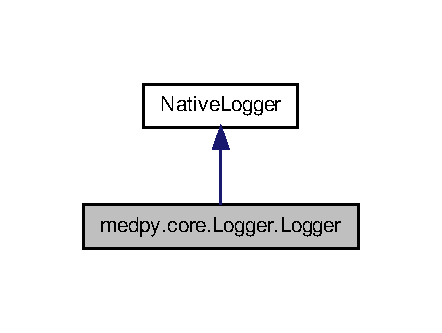
\includegraphics[width=212pt]{classmedpy_1_1core_1_1Logger_1_1Logger__inherit__graph}
\end{center}
\end{figure}


Collaboration diagram for medpy.core.Logger.Logger:\nopagebreak
\begin{figure}[H]
\begin{center}
\leavevmode
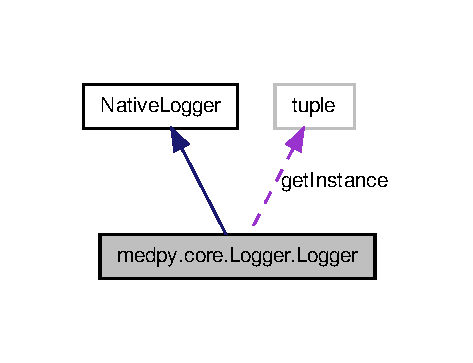
\includegraphics[width=227pt]{classmedpy_1_1core_1_1Logger_1_1Logger__coll__graph}
\end{center}
\end{figure}
\subsection*{Classes}
\begin{DoxyCompactItemize}
\item 
class \hyperlink{classmedpy_1_1core_1_1Logger_1_1Logger_1_1LoggerHelper}{LoggerHelper}
\begin{DoxyCompactList}\small\item\em A helper class which performs the actual initialization. \end{DoxyCompactList}\end{DoxyCompactItemize}
\subsection*{Public Member Functions}
\begin{DoxyCompactItemize}
\item 
\hypertarget{classmedpy_1_1core_1_1Logger_1_1Logger_a8fdfdb7972f6ca4f3b20e98985988bc7}{
def {\bfseries \_\-\_\-init\_\-\_\-}}
\label{classmedpy_1_1core_1_1Logger_1_1Logger_a8fdfdb7972f6ca4f3b20e98985988bc7}

\item 
def \hyperlink{classmedpy_1_1core_1_1Logger_1_1Logger_a9b4ca5d9e5d84d5da1ebda4929c3d757}{setHandler}
\begin{DoxyCompactList}\small\item\em Replaces the current handler with a new one. \end{DoxyCompactList}\item 
\hypertarget{classmedpy_1_1core_1_1Logger_1_1Logger_a7ef3cbfa57e61d02882e586ff7baa176}{
def \hyperlink{classmedpy_1_1core_1_1Logger_1_1Logger_a7ef3cbfa57e61d02882e586ff7baa176}{setLevel}}
\label{classmedpy_1_1core_1_1Logger_1_1Logger_a7ef3cbfa57e61d02882e586ff7baa176}

\begin{DoxyCompactList}\small\item\em Overrides the parent method to adapt the formatting string to the level. \end{DoxyCompactList}\end{DoxyCompactItemize}
\subsection*{Static Public Attributes}
\begin{DoxyCompactItemize}
\item 
\hypertarget{classmedpy_1_1core_1_1Logger_1_1Logger_ae169695a25c1a25f4929d03eb5ff016b}{
tuple {\bfseries getInstance} = \hyperlink{classmedpy_1_1core_1_1Logger_1_1Logger_1_1LoggerHelper}{LoggerHelper}()}
\label{classmedpy_1_1core_1_1Logger_1_1Logger_ae169695a25c1a25f4929d03eb5ff016b}

\end{DoxyCompactItemize}
\subsection*{Static Private Attributes}
\begin{DoxyCompactItemize}
\item 
\hypertarget{classmedpy_1_1core_1_1Logger_1_1Logger_af48b52980156fd81d4297cf243204a1e}{
{\bfseries \_\-instance} = None}
\label{classmedpy_1_1core_1_1Logger_1_1Logger_af48b52980156fd81d4297cf243204a1e}

\item 
\hypertarget{classmedpy_1_1core_1_1Logger_1_1Logger_a82158993b8453bc1b8881f5e92a413ff}{
{\bfseries \_\-handler} = None}
\label{classmedpy_1_1core_1_1Logger_1_1Logger_a82158993b8453bc1b8881f5e92a413ff}

\end{DoxyCompactItemize}


\subsection{Detailed Description}
This singleton class represents an object that can be used by all applications and classes. 

Definition at line 34 of file Logger.py.



\subsection{Member Function Documentation}
\hypertarget{classmedpy_1_1core_1_1Logger_1_1Logger_a9b4ca5d9e5d84d5da1ebda4929c3d757}{
\index{medpy::core::Logger::Logger@{medpy::core::Logger::Logger}!setHandler@{setHandler}}
\index{setHandler@{setHandler}!medpy::core::Logger::Logger@{medpy::core::Logger::Logger}}
\subsubsection[{setHandler}]{\setlength{\rightskip}{0pt plus 5cm}def medpy.core.Logger.Logger.setHandler (
\begin{DoxyParamCaption}
\item[{}]{self, }
\item[{}]{hdlr}
\end{DoxyParamCaption}
)}}
\label{classmedpy_1_1core_1_1Logger_1_1Logger_a9b4ca5d9e5d84d5da1ebda4929c3d757}


Replaces the current handler with a new one. 

If none should be replaces, but just one added, use the parent classes addHandler() method. 

Definition at line 76 of file Logger.py.



The documentation for this class was generated from the following file:\begin{DoxyCompactItemize}
\item 
/home/loli/Programming/Python/MedPy/src/medpy/core/Logger.py\end{DoxyCompactItemize}

\hypertarget{classmedpy_1_1core_1_1Logger_1_1Logger_1_1LoggerHelper}{
\section{medpy.core.Logger.Logger.LoggerHelper Class Reference}
\label{classmedpy_1_1core_1_1Logger_1_1Logger_1_1LoggerHelper}\index{medpy::core::Logger::Logger::LoggerHelper@{medpy::core::Logger::Logger::LoggerHelper}}
}


A helper class which performs the actual initialization.  




Inheritance diagram for medpy.core.Logger.Logger.LoggerHelper:\nopagebreak
\begin{figure}[H]
\begin{center}
\leavevmode
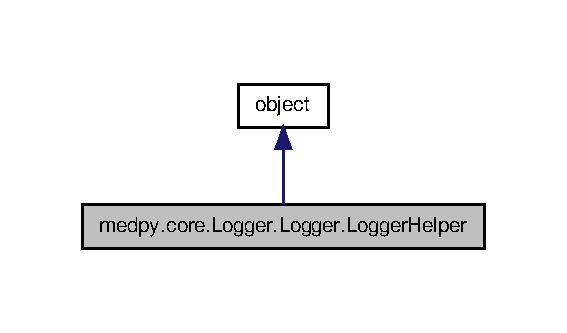
\includegraphics[width=272pt]{classmedpy_1_1core_1_1Logger_1_1Logger_1_1LoggerHelper__inherit__graph}
\end{center}
\end{figure}


Collaboration diagram for medpy.core.Logger.Logger.LoggerHelper:\nopagebreak
\begin{figure}[H]
\begin{center}
\leavevmode
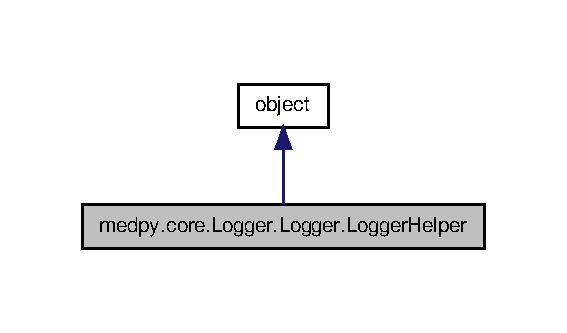
\includegraphics[width=272pt]{classmedpy_1_1core_1_1Logger_1_1Logger_1_1LoggerHelper__coll__graph}
\end{center}
\end{figure}
\subsection*{Public Member Functions}
\begin{DoxyCompactItemize}
\item 
\hypertarget{classmedpy_1_1core_1_1Logger_1_1Logger_1_1LoggerHelper_aea5d63b929cd6340bc6f8f249956e44b}{
def {\bfseries \_\-\_\-call\_\-\_\-}}
\label{classmedpy_1_1core_1_1Logger_1_1Logger_1_1LoggerHelper_aea5d63b929cd6340bc6f8f249956e44b}

\end{DoxyCompactItemize}


\subsection{Detailed Description}
A helper class which performs the actual initialization. 

Definition at line 40 of file Logger.py.



The documentation for this class was generated from the following file:\begin{DoxyCompactItemize}
\item 
/home/loli/Programming/Python/MedPy/src/medpy/core/Logger.py\end{DoxyCompactItemize}

\hypertarget{classNativeLogger}{
\section{NativeLogger Class Reference}
\label{classNativeLogger}\index{NativeLogger@{NativeLogger}}
}


Inheritance diagram for NativeLogger:\nopagebreak
\begin{figure}[H]
\begin{center}
\leavevmode
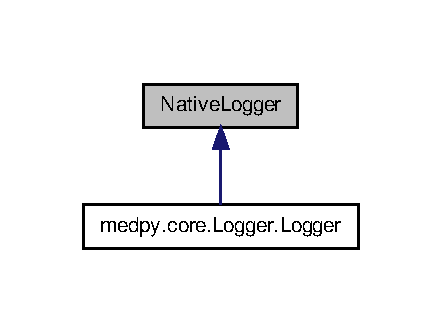
\includegraphics[width=212pt]{classNativeLogger__inherit__graph}
\end{center}
\end{figure}


The documentation for this class was generated from the following file:\begin{DoxyCompactItemize}
\item 
/home/loli/Programming/Python/MedPy/src/medpy/core/Logger.py\end{DoxyCompactItemize}

\hypertarget{classobject}{
\section{object Class Reference}
\label{classobject}\index{object@{object}}
}


Inheritance diagram for object:\nopagebreak
\begin{figure}[H]
\begin{center}
\leavevmode
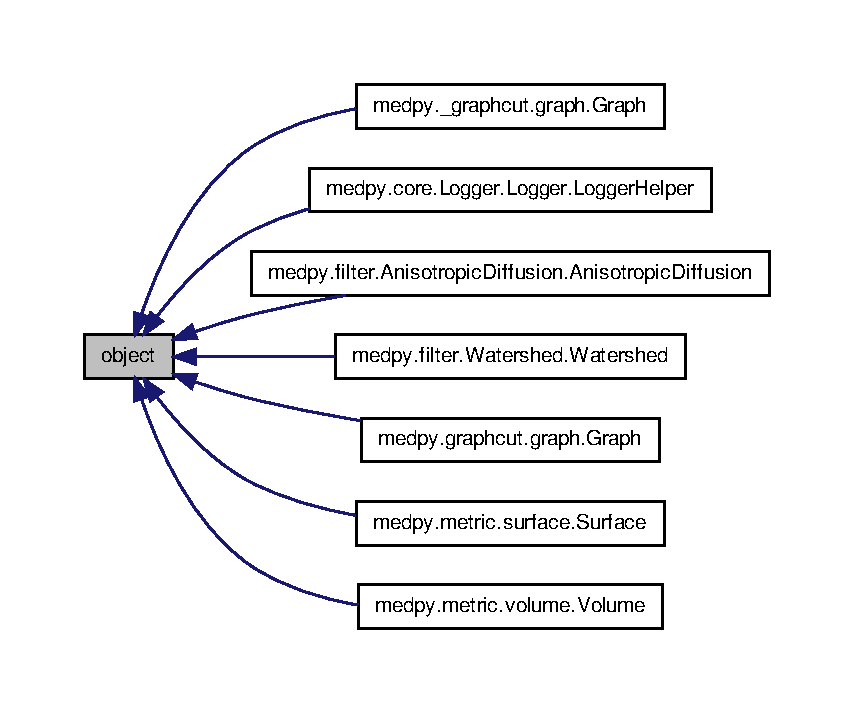
\includegraphics[width=400pt]{classobject__inherit__graph}
\end{center}
\end{figure}


The documentation for this class was generated from the following file:\begin{DoxyCompactItemize}
\item 
/home/omaier/Programming/Python/medpy/src/medpy/filter/AnisotropicDiffusion.py\end{DoxyCompactItemize}

\hypertarget{classmedpy_1_1core_1_1exceptions_1_1SubprocessError}{
\section{medpy.core.exceptions.SubprocessError Class Reference}
\label{classmedpy_1_1core_1_1exceptions_1_1SubprocessError}\index{medpy::core::exceptions::SubprocessError@{medpy::core::exceptions::SubprocessError}}
}


Thrown by an application when a subprocess execution failed.  




Inheritance diagram for medpy.core.exceptions.SubprocessError:\nopagebreak
\begin{figure}[H]
\begin{center}
\leavevmode
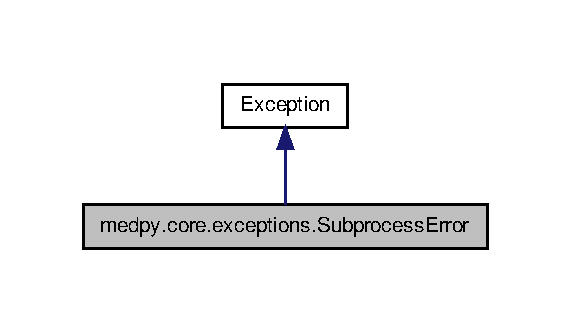
\includegraphics[width=274pt]{classmedpy_1_1core_1_1exceptions_1_1SubprocessError__inherit__graph}
\end{center}
\end{figure}


Collaboration diagram for medpy.core.exceptions.SubprocessError:\nopagebreak
\begin{figure}[H]
\begin{center}
\leavevmode
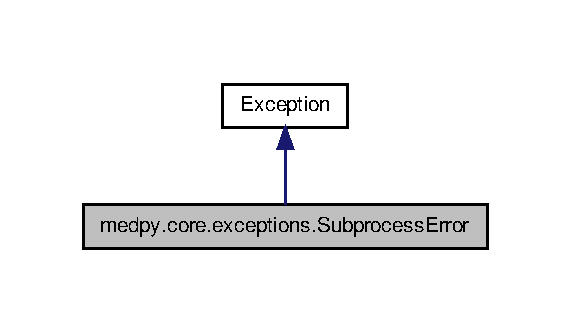
\includegraphics[width=274pt]{classmedpy_1_1core_1_1exceptions_1_1SubprocessError__coll__graph}
\end{center}
\end{figure}


\subsection{Detailed Description}
Thrown by an application when a subprocess execution failed. 

Definition at line 44 of file exceptions.py.



The documentation for this class was generated from the following file:\begin{DoxyCompactItemize}
\item 
/home/omaier/Programming/Python/medpy/src/medpy/core/exceptions.py\end{DoxyCompactItemize}

\hypertarget{classmedpy_1_1metric_1_1surface_1_1Surface}{
\section{medpy.metric.surface.Surface Class Reference}
\label{classmedpy_1_1metric_1_1surface_1_1Surface}\index{medpy::metric::surface::Surface@{medpy::metric::surface::Surface}}
}


Computes different surface metrics between two 3D-\/images contain each an object.  




Inheritance diagram for medpy.metric.surface.Surface:\nopagebreak
\begin{figure}[H]
\begin{center}
\leavevmode
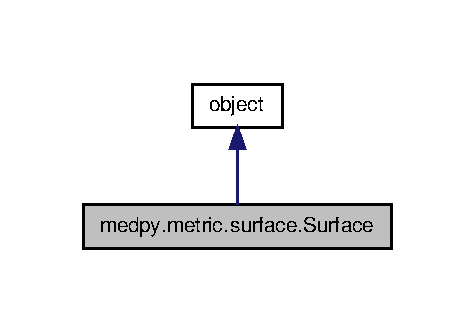
\includegraphics[width=228pt]{classmedpy_1_1metric_1_1surface_1_1Surface__inherit__graph}
\end{center}
\end{figure}


Collaboration diagram for medpy.metric.surface.Surface:\nopagebreak
\begin{figure}[H]
\begin{center}
\leavevmode
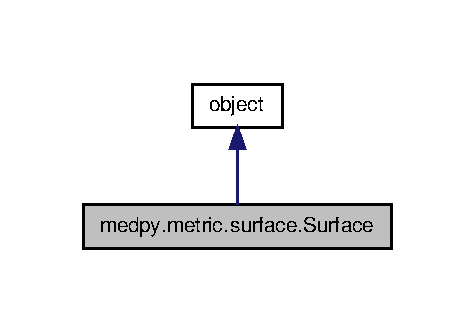
\includegraphics[width=228pt]{classmedpy_1_1metric_1_1surface_1_1Surface__coll__graph}
\end{center}
\end{figure}
\subsection*{Public Member Functions}
\begin{DoxyCompactItemize}
\item 
def \hyperlink{classmedpy_1_1metric_1_1surface_1_1Surface_a46994eacbac664bc6d33d19bac6f7b2c}{\_\-\_\-init\_\-\_\-}
\begin{DoxyCompactList}\small\item\em Initialize the class with two binary images, each containing a single object. \end{DoxyCompactList}\item 
def \hyperlink{classmedpy_1_1metric_1_1surface_1_1Surface_a8684d8c1382318e6bf319b668c81dd1a}{get\_\-maximum\_\-symmetric\_\-surface\_\-distance}
\begin{DoxyCompactList}\small\item\em Computes the maximum symmetric surface distance, also known as Hausdorff distance, between the two objects surfaces. \end{DoxyCompactList}\item 
def \hyperlink{classmedpy_1_1metric_1_1surface_1_1Surface_a920a84703f013d3c30b9a29e352700d9}{get\_\-root\_\-mean\_\-square\_\-symmetric\_\-surface\_\-distance}
\begin{DoxyCompactList}\small\item\em Computes the root mean square symmetric surface distance between the two objects surfaces. \end{DoxyCompactList}\item 
def \hyperlink{classmedpy_1_1metric_1_1surface_1_1Surface_a1f0c6c294baebf0ca8f45c47697e6410}{get\_\-average\_\-symmetric\_\-surface\_\-distance}
\begin{DoxyCompactList}\small\item\em Computes the average symmetric surface distance between the two objects surfaces. \end{DoxyCompactList}\item 
def \hyperlink{classmedpy_1_1metric_1_1surface_1_1Surface_a24fed896ac83b61f7abd9719ebe8ff6f}{get\_\-mask\_\-reference\_\-nn}
\item 
def \hyperlink{classmedpy_1_1metric_1_1surface_1_1Surface_abbd8cea3e3dd7a4a9c1af123e889e7bb}{get\_\-reference\_\-mask\_\-nn}
\item 
def \hyperlink{classmedpy_1_1metric_1_1surface_1_1Surface_adf21c517a7f9cfc187546e2c2db99409}{get\_\-mask\_\-edge\_\-points}
\item 
def \hyperlink{classmedpy_1_1metric_1_1surface_1_1Surface_abee40ce81906de3f356a08019985be24}{get\_\-reference\_\-edge\_\-points}
\end{DoxyCompactItemize}
\paragraph*{}
\begin{DoxyCompactItemize}
\item 
def \hyperlink{classmedpy_1_1metric_1_1surface_1_1Surface_aee3d28744eeac497b32362ba5ef9f8bb}{compute\_\-contour}
\begin{DoxyCompactList}\small\item\em Uses a 18-\/neighbourhood filter to create an edge image of the input object. \end{DoxyCompactList}\end{DoxyCompactItemize}



\subsection{Detailed Description}
Computes different surface metrics between two 3D-\/images contain each an object. 

The surface of the objects is computed using a 18-\/neighbourhood edge detection. The distance metrics are computed over all points of the surfaces using the nearest neighbour approach. Beside this provides a number of statistics of the two images.

During the initialization the edge detection is run for both images, taking up to 5 min (on 512$^\wedge$3 images). The first call to one of the metric measures triggers the computation of the nearest neighbours, taking up to 7 minutes (based on 250.000 edge point for each of the objects, which corresponds to a typical liver mask). All subsequent calls to one of the metrics measures can be expected be in the sub-\/millisecond area.

Metrics defined in: Heimann, T.; van Ginneken, B.; Styner, M.A.; Arzhaeva, Y.; Aurich, V.; Bauer, C.; Beck, A.; Becker, C.; Beichel, R.; Bekes, G.; Bello, F.; Binnig, G.; Bischof, H.; Bornik, A.; Cashman, P.; Ying Chi; Cordova, A.; Dawant, B.M.; Fidrich, M.; Furst, J.D.; Furukawa, D.; Grenacher, L.; Hornegger, J.; Kainmuller, D.; Kitney, R.I.; Kobatake, H.; Lamecker, H.; Lange, T.; Jeongjin Lee; Lennon, B.; Rui Li; Senhu Li; Meinzer, H.-\/P.; Nemeth, G.; Raicu, D.S.; Rau, A.-\/M.; van Rikxoort, E.M.; Rousson, M.; Rusko, L.; Saddi, K.A.; Schmidt, G.; Seghers, D.; Shimizu, A.; Slagmolen, P.; Sorantin, E.; Soza, G.; Susomboon, R.; Waite, J.M.; Wimmer, A.; Wolf, I.; , \char`\"{}Comparison and Evaluation of Methods for Liver Segmentation From CT Datasets,\char`\"{} Medical Imaging, IEEE Transactions on , vol.28, no.8, pp.1251-\/1265, Aug. 2009 doi: 10.1109/TMI.2009.2013851 

Definition at line 44 of file surface.py.



\subsection{Constructor \& Destructor Documentation}
\hypertarget{classmedpy_1_1metric_1_1surface_1_1Surface_a46994eacbac664bc6d33d19bac6f7b2c}{
\index{medpy::metric::surface::Surface@{medpy::metric::surface::Surface}!\_\-\_\-init\_\-\_\-@{\_\-\_\-init\_\-\_\-}}
\index{\_\-\_\-init\_\-\_\-@{\_\-\_\-init\_\-\_\-}!medpy::metric::surface::Surface@{medpy::metric::surface::Surface}}
\subsubsection[{\_\-\_\-init\_\-\_\-}]{\setlength{\rightskip}{0pt plus 5cm}def medpy.metric.surface.Surface.\_\-\_\-init\_\-\_\- (
\begin{DoxyParamCaption}
\item[{}]{self, }
\item[{}]{mask, }
\item[{}]{reference, }
\item[{}]{physical\_\-voxel\_\-spacing = {\ttfamily \mbox{[}1}, }
\item[{}]{mask\_\-offset = {\ttfamily \mbox{[}0}, }
\item[{}]{reference\_\-offset = {\ttfamily \mbox{[}0}}
\end{DoxyParamCaption}
)}}
\label{classmedpy_1_1metric_1_1surface_1_1Surface_a46994eacbac664bc6d33d19bac6f7b2c}


Initialize the class with two binary images, each containing a single object. 

Assumes the input to be a representation of a 3D image, that fits one of the following formats:
\begin{DoxyItemize}
\item 1. all 0 values denoting background, all others the foreground/object
\item 2. all False values denoting the background, all others the foreground/object The first image passed is referred to as 'mask', the second as 'reference'. This is only important for some metrics that are not symmetric (and therefore not really metrics). 
\begin{DoxyParams}{Parameters}
{\em mask} & binary mask as an scipy array (3D image) \\
\hline
{\em reference} & binary reference as an scipy array (3D image) \\
\hline
{\em physical\_\-voxel\_\-spacing} & The physical voxel spacing of the two images (must be the same for both) \\
\hline
{\em mask\_\-offset} & offset of the mask array to 0,0,0-\/origin \\
\hline
{\em reference\_\-offset} & offset of the reference array to 0,0,0-\/origin \\
\hline
\end{DoxyParams}

\end{DoxyItemize}

Definition at line 74 of file surface.py.



\subsection{Member Function Documentation}
\hypertarget{classmedpy_1_1metric_1_1surface_1_1Surface_aee3d28744eeac497b32362ba5ef9f8bb}{
\index{medpy::metric::surface::Surface@{medpy::metric::surface::Surface}!compute\_\-contour@{compute\_\-contour}}
\index{compute\_\-contour@{compute\_\-contour}!medpy::metric::surface::Surface@{medpy::metric::surface::Surface}}
\subsubsection[{compute\_\-contour}]{\setlength{\rightskip}{0pt plus 5cm}def medpy.metric.surface.Surface.compute\_\-contour (
\begin{DoxyParamCaption}
\item[{}]{array}
\end{DoxyParamCaption}
)}}
\label{classmedpy_1_1metric_1_1surface_1_1Surface_aee3d28744eeac497b32362ba5ef9f8bb}


Uses a 18-\/neighbourhood filter to create an edge image of the input object. 

Assumes the input to be a representation of a 3D image, that fits one of the following formats:
\begin{DoxyItemize}
\item 1. all 0 values denoting background, all others the foreground/object
\item 2. all False values denoting the background, all others the foreground/object The area outside the array is assumed to contain background voxels. The method does not ensure that the object voxels are actually connected, this is silently assumed.
\end{DoxyItemize}


\begin{DoxyParams}{Parameters}
{\em array} & a numpy array with only 0/N0\} or False/True values. \\
\hline
\end{DoxyParams}
\begin{DoxyReturn}{Returns}
a boolean numpy array with the input objects edges 
\end{DoxyReturn}


Definition at line 295 of file surface.py.

\hypertarget{classmedpy_1_1metric_1_1surface_1_1Surface_a1f0c6c294baebf0ca8f45c47697e6410}{
\index{medpy::metric::surface::Surface@{medpy::metric::surface::Surface}!get\_\-average\_\-symmetric\_\-surface\_\-distance@{get\_\-average\_\-symmetric\_\-surface\_\-distance}}
\index{get\_\-average\_\-symmetric\_\-surface\_\-distance@{get\_\-average\_\-symmetric\_\-surface\_\-distance}!medpy::metric::surface::Surface@{medpy::metric::surface::Surface}}
\subsubsection[{get\_\-average\_\-symmetric\_\-surface\_\-distance}]{\setlength{\rightskip}{0pt plus 5cm}def medpy.metric.surface.Surface.get\_\-average\_\-symmetric\_\-surface\_\-distance (
\begin{DoxyParamCaption}
\item[{}]{self}
\end{DoxyParamCaption}
)}}
\label{classmedpy_1_1metric_1_1surface_1_1Surface_a1f0c6c294baebf0ca8f45c47697e6410}


Computes the average symmetric surface distance between the two objects surfaces. 

\begin{DoxyReturn}{Returns}
average symmetric surface distance in millimeters
\end{DoxyReturn}
For a perfect segmentation this distance is 0.

Metric definition: Let $S(A)$ denote the set of surface voxels of $A$. The shortest distance of an arbitrary voxel $v$ to $S(A)$ is defined as: \[ d(v,S(A)) = \min_{s_A\in S(A)} ||v-s_A|| \] where $||.||$ denotes the Euclidean distance. The average symmetric surface distance is then given by: \[ ASD(A,B) = \frac{1}{|S(A)|+|S(B)|} \left( \sum_{s_A\in S(A)} d(s_A,S(B)) + \sum_{s_B\in S(B)} d(s_B,S(A)) \right) \] 

Definition at line 218 of file surface.py.

\hypertarget{classmedpy_1_1metric_1_1surface_1_1Surface_adf21c517a7f9cfc187546e2c2db99409}{
\index{medpy::metric::surface::Surface@{medpy::metric::surface::Surface}!get\_\-mask\_\-edge\_\-points@{get\_\-mask\_\-edge\_\-points}}
\index{get\_\-mask\_\-edge\_\-points@{get\_\-mask\_\-edge\_\-points}!medpy::metric::surface::Surface@{medpy::metric::surface::Surface}}
\subsubsection[{get\_\-mask\_\-edge\_\-points}]{\setlength{\rightskip}{0pt plus 5cm}def medpy.metric.surface.Surface.get\_\-mask\_\-edge\_\-points (
\begin{DoxyParamCaption}
\item[{}]{self}
\end{DoxyParamCaption}
)}}
\label{classmedpy_1_1metric_1_1surface_1_1Surface_adf21c517a7f9cfc187546e2c2db99409}
\begin{DoxyReturn}{Returns}
The edge points of the mask object. 
\end{DoxyReturn}


Definition at line 270 of file surface.py.

\hypertarget{classmedpy_1_1metric_1_1surface_1_1Surface_a24fed896ac83b61f7abd9719ebe8ff6f}{
\index{medpy::metric::surface::Surface@{medpy::metric::surface::Surface}!get\_\-mask\_\-reference\_\-nn@{get\_\-mask\_\-reference\_\-nn}}
\index{get\_\-mask\_\-reference\_\-nn@{get\_\-mask\_\-reference\_\-nn}!medpy::metric::surface::Surface@{medpy::metric::surface::Surface}}
\subsubsection[{get\_\-mask\_\-reference\_\-nn}]{\setlength{\rightskip}{0pt plus 5cm}def medpy.metric.surface.Surface.get\_\-mask\_\-reference\_\-nn (
\begin{DoxyParamCaption}
\item[{}]{self}
\end{DoxyParamCaption}
)}}
\label{classmedpy_1_1metric_1_1surface_1_1Surface_a24fed896ac83b61f7abd9719ebe8ff6f}
\begin{DoxyReturn}{Returns}
The distances of the nearest neighbours of all mask edge points to all reference edge points. 
\end{DoxyReturn}


Definition at line 239 of file surface.py.

\hypertarget{classmedpy_1_1metric_1_1surface_1_1Surface_a8684d8c1382318e6bf319b668c81dd1a}{
\index{medpy::metric::surface::Surface@{medpy::metric::surface::Surface}!get\_\-maximum\_\-symmetric\_\-surface\_\-distance@{get\_\-maximum\_\-symmetric\_\-surface\_\-distance}}
\index{get\_\-maximum\_\-symmetric\_\-surface\_\-distance@{get\_\-maximum\_\-symmetric\_\-surface\_\-distance}!medpy::metric::surface::Surface@{medpy::metric::surface::Surface}}
\subsubsection[{get\_\-maximum\_\-symmetric\_\-surface\_\-distance}]{\setlength{\rightskip}{0pt plus 5cm}def medpy.metric.surface.Surface.get\_\-maximum\_\-symmetric\_\-surface\_\-distance (
\begin{DoxyParamCaption}
\item[{}]{self}
\end{DoxyParamCaption}
)}}
\label{classmedpy_1_1metric_1_1surface_1_1Surface_a8684d8c1382318e6bf319b668c81dd1a}


Computes the maximum symmetric surface distance, also known as Hausdorff distance, between the two objects surfaces. 

\begin{DoxyReturn}{Returns}
the maximum symmetric surface distance in millimeters
\end{DoxyReturn}
For a perfect segmentation this distance is 0. This metric is sensitive to outliers and returns the true maximum error.

Metric definition: Let $S(A)$ denote the set of surface voxels of $A$. The shortest distance of an arbitrary voxel $v$ to $S(A)$ is defined as: \[ d(v,S(A)) = \min_{s_A\in S(A)} ||v-s_A|| \] where $||.||$ denotes the Euclidean distance. The maximum symmetric surface distance is then given by: \[ MSD(A,B) = \max \left\{ \max_{s_A\in S(A)} d(s_A,S(B)), \max_{s_B\in S(B)} d(s_B,S(A)), \right\} \] 

Definition at line 133 of file surface.py.

\hypertarget{classmedpy_1_1metric_1_1surface_1_1Surface_abee40ce81906de3f356a08019985be24}{
\index{medpy::metric::surface::Surface@{medpy::metric::surface::Surface}!get\_\-reference\_\-edge\_\-points@{get\_\-reference\_\-edge\_\-points}}
\index{get\_\-reference\_\-edge\_\-points@{get\_\-reference\_\-edge\_\-points}!medpy::metric::surface::Surface@{medpy::metric::surface::Surface}}
\subsubsection[{get\_\-reference\_\-edge\_\-points}]{\setlength{\rightskip}{0pt plus 5cm}def medpy.metric.surface.Surface.get\_\-reference\_\-edge\_\-points (
\begin{DoxyParamCaption}
\item[{}]{self}
\end{DoxyParamCaption}
)}}
\label{classmedpy_1_1metric_1_1surface_1_1Surface_abee40ce81906de3f356a08019985be24}
\begin{DoxyReturn}{Returns}
The edge points of the reference object. 
\end{DoxyReturn}


Definition at line 277 of file surface.py.

\hypertarget{classmedpy_1_1metric_1_1surface_1_1Surface_abbd8cea3e3dd7a4a9c1af123e889e7bb}{
\index{medpy::metric::surface::Surface@{medpy::metric::surface::Surface}!get\_\-reference\_\-mask\_\-nn@{get\_\-reference\_\-mask\_\-nn}}
\index{get\_\-reference\_\-mask\_\-nn@{get\_\-reference\_\-mask\_\-nn}!medpy::metric::surface::Surface@{medpy::metric::surface::Surface}}
\subsubsection[{get\_\-reference\_\-mask\_\-nn}]{\setlength{\rightskip}{0pt plus 5cm}def medpy.metric.surface.Surface.get\_\-reference\_\-mask\_\-nn (
\begin{DoxyParamCaption}
\item[{}]{self}
\end{DoxyParamCaption}
)}}
\label{classmedpy_1_1metric_1_1surface_1_1Surface_abbd8cea3e3dd7a4a9c1af123e889e7bb}
\begin{DoxyReturn}{Returns}
The distances of the nearest neighbours of all reference edge points to all mask edge points.
\end{DoxyReturn}
The underlying algorithm used for the scipy.spatial.KDTree implementation is based on: Sunil Arya, David M. Mount, Nathan S. Netanyahu, Ruth Silverman, and Angela Y. Wu. 1998. An optimal algorithm for approximate nearest neighbor searching fixed dimensions. J. ACM 45, 6 (November 1998), 891-\/923 

Definition at line 257 of file surface.py.

\hypertarget{classmedpy_1_1metric_1_1surface_1_1Surface_a920a84703f013d3c30b9a29e352700d9}{
\index{medpy::metric::surface::Surface@{medpy::metric::surface::Surface}!get\_\-root\_\-mean\_\-square\_\-symmetric\_\-surface\_\-distance@{get\_\-root\_\-mean\_\-square\_\-symmetric\_\-surface\_\-distance}}
\index{get\_\-root\_\-mean\_\-square\_\-symmetric\_\-surface\_\-distance@{get\_\-root\_\-mean\_\-square\_\-symmetric\_\-surface\_\-distance}!medpy::metric::surface::Surface@{medpy::metric::surface::Surface}}
\subsubsection[{get\_\-root\_\-mean\_\-square\_\-symmetric\_\-surface\_\-distance}]{\setlength{\rightskip}{0pt plus 5cm}def medpy.metric.surface.Surface.get\_\-root\_\-mean\_\-square\_\-symmetric\_\-surface\_\-distance (
\begin{DoxyParamCaption}
\item[{}]{self}
\end{DoxyParamCaption}
)}}
\label{classmedpy_1_1metric_1_1surface_1_1Surface_a920a84703f013d3c30b9a29e352700d9}


Computes the root mean square symmetric surface distance between the two objects surfaces. 

\begin{DoxyReturn}{Returns}
root mean square symmetric surface distance in millimeters
\end{DoxyReturn}
For a perfect segmentation this distance is 0. This metric punishes large deviations from the true contour stronger than the average symmetric surface distance.

Metric definition: Let $S(A)$ denote the set of surface voxels of $A$. The shortest distance of an arbitrary voxel $v$ to $S(A)$ is defined as: \[ d(v,S(A)) = \min_{s_A\in S(A)} ||v-s_A|| \] where $||.||$ denotes the Euclidean distance. The root mean square symmetric surface distance is then given by: \[ RMSD(A,B) = \sqrt{\frac{1}{|S(A)|+|S(B)|}} \times \sqrt{ \sum_{s_A\in S(A)} d^2(s_A,S(B)) + \sum_{s_B\in S(B)} d^2(s_B,S(A)) } \] 

Definition at line 171 of file surface.py.



The documentation for this class was generated from the following file:\begin{DoxyCompactItemize}
\item 
/home/omaier/Programming/Python/medpy/src/medpy/metric/surface.py\end{DoxyCompactItemize}

\hypertarget{classunittest_1_1TestCase}{
\section{TestCase Class Reference}
\label{classunittest_1_1TestCase}\index{unittest::TestCase@{unittest::TestCase}}
}


Inheritance diagram for TestCase:\nopagebreak
\begin{figure}[H]
\begin{center}
\leavevmode
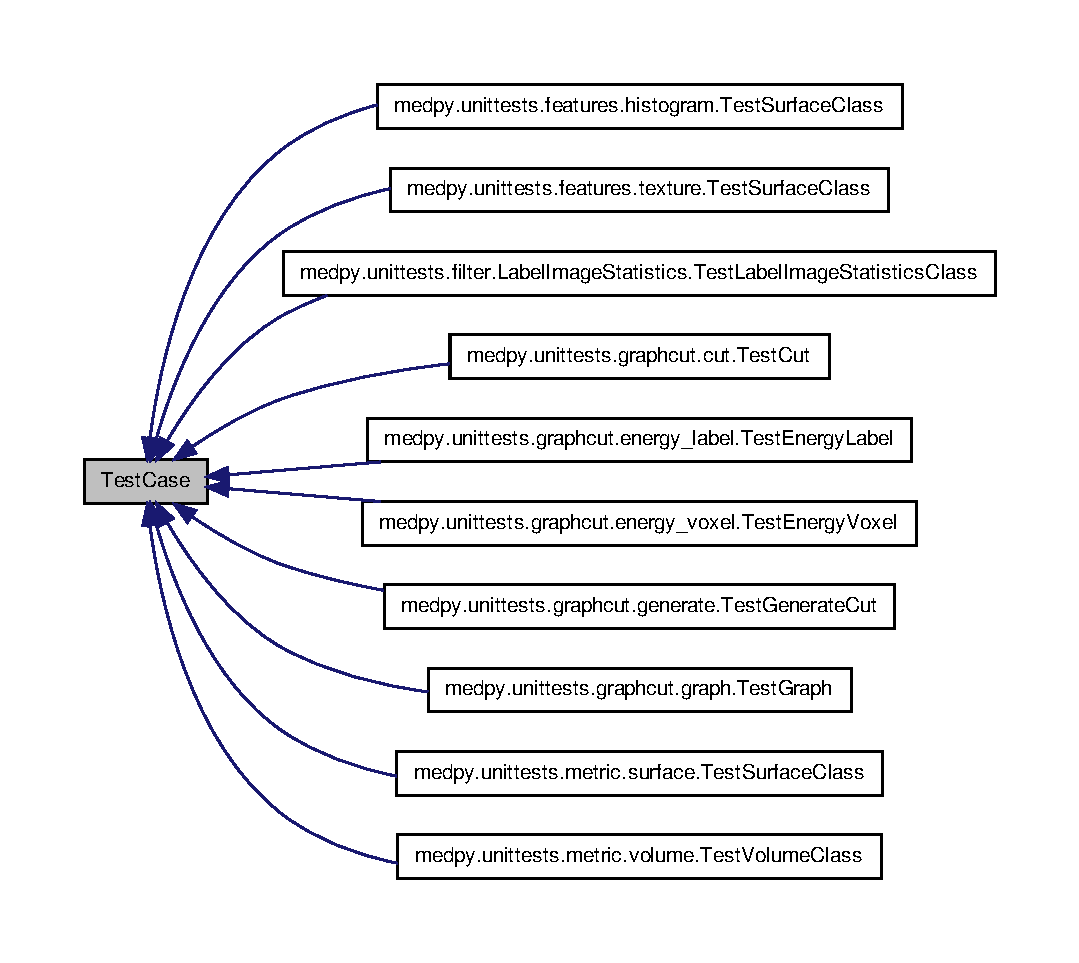
\includegraphics[width=400pt]{classunittest_1_1TestCase__inherit__graph}
\end{center}
\end{figure}


The documentation for this class was generated from the following file:\begin{DoxyCompactItemize}
\item 
/home/loli/Programming/Python/MedPy/src/medpy/tests/metric/Surface.py\end{DoxyCompactItemize}

\hypertarget{classmedpy_1_1unittests_1_1graphcut_1_1graph_1_1TestGraph}{
\section{medpy.unittests.graphcut.graph.TestGraph Class Reference}
\label{classmedpy_1_1unittests_1_1graphcut_1_1graph_1_1TestGraph}\index{medpy::unittests::graphcut::graph::TestGraph@{medpy::unittests::graphcut::graph::TestGraph}}
}


Inheritance diagram for medpy.unittests.graphcut.graph.TestGraph:\nopagebreak
\begin{figure}[H]
\begin{center}
\leavevmode
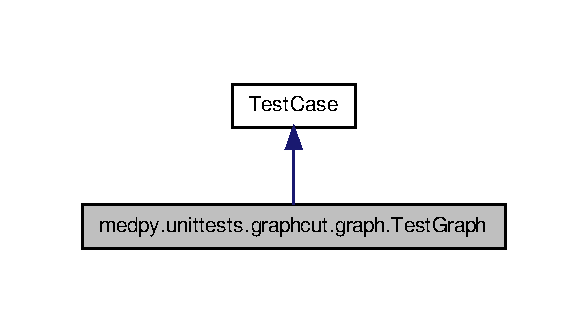
\includegraphics[width=282pt]{classmedpy_1_1unittests_1_1graphcut_1_1graph_1_1TestGraph__inherit__graph}
\end{center}
\end{figure}


Collaboration diagram for medpy.unittests.graphcut.graph.TestGraph:\nopagebreak
\begin{figure}[H]
\begin{center}
\leavevmode
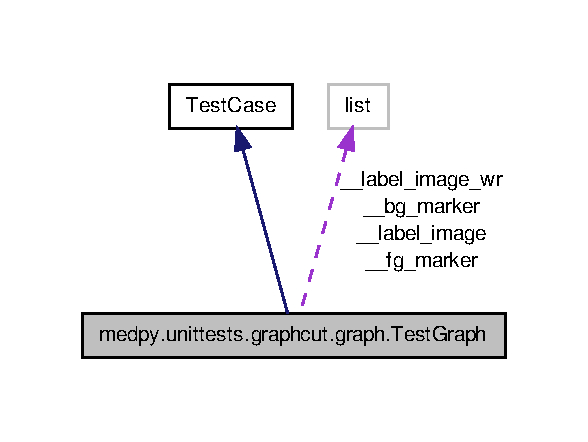
\includegraphics[width=282pt]{classmedpy_1_1unittests_1_1graphcut_1_1graph_1_1TestGraph__coll__graph}
\end{center}
\end{figure}
\subsection*{Public Member Functions}
\begin{DoxyCompactItemize}
\item 
\hypertarget{classmedpy_1_1unittests_1_1graphcut_1_1graph_1_1TestGraph_a19d5a3f0c6ccd4586e5467f2c5872c96}{
def \hyperlink{classmedpy_1_1unittests_1_1graphcut_1_1graph_1_1TestGraph_a19d5a3f0c6ccd4586e5467f2c5872c96}{test\_\-graph\_\-from\_\-labels\_\-w\_\-boundary}}
\label{classmedpy_1_1unittests_1_1graphcut_1_1graph_1_1TestGraph_a19d5a3f0c6ccd4586e5467f2c5872c96}

\begin{DoxyCompactList}\small\item\em Tests the \hyperlink{}{function using a boundary term and no regional term. }\end{DoxyCompactList}\item 
def \hyperlink{classmedpy_1_1unittests_1_1graphcut_1_1graph_1_1TestGraph_ac50662dfbbba6e7a7f740eb3f63e64e7}{test\_\-graph\_\-from\_\-labels\_\-nd}
\begin{DoxyCompactList}\small\item\em Check the multi-\/dimensional capabilities of \hyperlink{}{up to the fourth dimension. }\end{DoxyCompactList}\end{DoxyCompactItemize}


\subsection{Detailed Description}


Definition at line 21 of file graph.py.



\subsection{Member Function Documentation}
\hypertarget{classmedpy_1_1unittests_1_1graphcut_1_1graph_1_1TestGraph_ac50662dfbbba6e7a7f740eb3f63e64e7}{
\index{medpy::unittests::graphcut::graph::TestGraph@{medpy::unittests::graphcut::graph::TestGraph}!test\_\-graph\_\-from\_\-labels\_\-nd@{test\_\-graph\_\-from\_\-labels\_\-nd}}
\index{test\_\-graph\_\-from\_\-labels\_\-nd@{test\_\-graph\_\-from\_\-labels\_\-nd}!medpy::unittests::graphcut::graph::TestGraph@{medpy::unittests::graphcut::graph::TestGraph}}
\subsubsection[{test\_\-graph\_\-from\_\-labels\_\-nd}]{\setlength{\rightskip}{0pt plus 5cm}def medpy.unittests.graphcut.graph.TestGraph.test\_\-graph\_\-from\_\-labels\_\-nd (
\begin{DoxyParamCaption}
\item[{}]{self}
\end{DoxyParamCaption}
)}}
\label{classmedpy_1_1unittests_1_1graphcut_1_1graph_1_1TestGraph_ac50662dfbbba6e7a7f740eb3f63e64e7}


Check the multi-\/dimensional capabilities of \hyperlink{}{up to the fourth dimension. }

(assuming ndim$\ast$2-\/connectedness) 

Definition at line 112 of file graph.py.



The documentation for this class was generated from the following file:\begin{DoxyCompactItemize}
\item 
/home/omaier/Programming/Python/medpy/src/medpy/unittests/graphcut/graph.py\end{DoxyCompactItemize}

\hypertarget{classmedpy_1_1unittests_1_1filter_1_1LabelImageStatistics_1_1TestLabelImageStatisticsClass}{
\section{medpy.unittests.filter.LabelImageStatistics.TestLabelImageStatisticsClass Class Reference}
\label{classmedpy_1_1unittests_1_1filter_1_1LabelImageStatistics_1_1TestLabelImageStatisticsClass}\index{medpy::unittests::filter::LabelImageStatistics::TestLabelImageStatisticsClass@{medpy::unittests::filter::LabelImageStatistics::TestLabelImageStatisticsClass}}
}


Inheritance diagram for medpy.unittests.filter.LabelImageStatistics.TestLabelImageStatisticsClass:\nopagebreak
\begin{figure}[H]
\begin{center}
\leavevmode
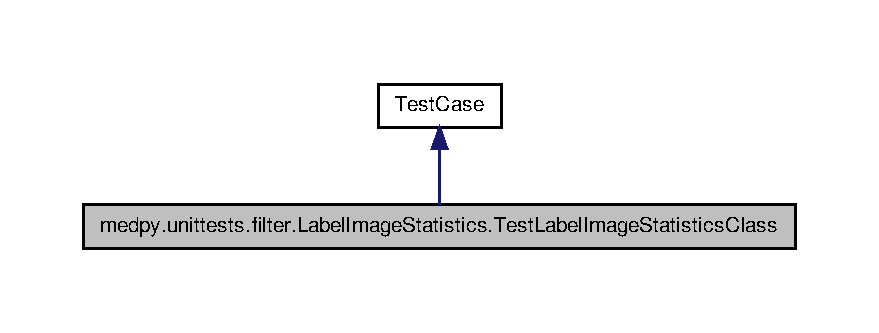
\includegraphics[width=400pt]{classmedpy_1_1unittests_1_1filter_1_1LabelImageStatistics_1_1TestLabelImageStatisticsClass__inherit__graph}
\end{center}
\end{figure}


Collaboration diagram for medpy.unittests.filter.LabelImageStatistics.TestLabelImageStatisticsClass:\nopagebreak
\begin{figure}[H]
\begin{center}
\leavevmode
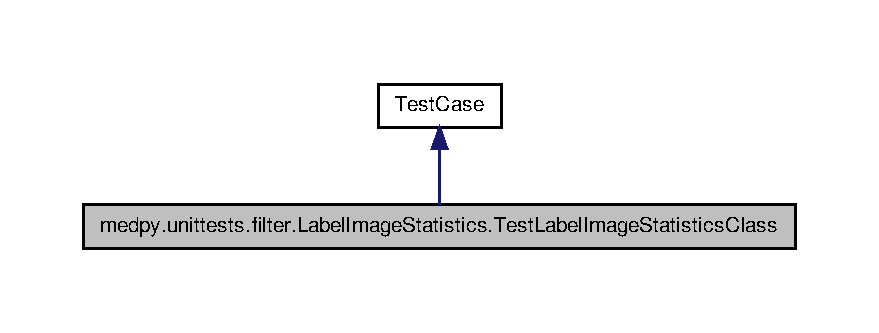
\includegraphics[width=400pt]{classmedpy_1_1unittests_1_1filter_1_1LabelImageStatistics_1_1TestLabelImageStatisticsClass__coll__graph}
\end{center}
\end{figure}
\subsection*{Public Member Functions}
\begin{DoxyCompactItemize}
\item 
def \hyperlink{classmedpy_1_1unittests_1_1filter_1_1LabelImageStatistics_1_1TestLabelImageStatisticsClass_a11774eb7b34a0b57706f900ada133e6c}{test\_\-Basic}
\begin{DoxyCompactList}\small\item\em Test the case of a region with only one intensity value and some basic return values. \end{DoxyCompactList}\item 
def \hyperlink{classmedpy_1_1unittests_1_1filter_1_1LabelImageStatistics_1_1TestLabelImageStatisticsClass_a1d0ee16f881a31e630361188b95e0b67}{test\_\-Homogeneous}
\begin{DoxyCompactList}\small\item\em Checks the return value for a homogeneous region. \end{DoxyCompactList}\item 
def \hyperlink{classmedpy_1_1unittests_1_1filter_1_1LabelImageStatistics_1_1TestLabelImageStatisticsClass_aec02bcfd0d2094a05786a87d0f6c2f65}{test\_\-Equality}
\begin{DoxyCompactList}\small\item\em Checks whether equally formed histograms in different intensity regions produce the same result. \end{DoxyCompactList}\item 
def \hyperlink{classmedpy_1_1unittests_1_1filter_1_1LabelImageStatistics_1_1TestLabelImageStatisticsClass_aa2077eec84a00d739c7f37ade7cf8780}{test\_\-Continuity}
\begin{DoxyCompactList}\small\item\em Checks if the returned values are continuous for more spaced intensity values. \end{DoxyCompactList}\item 
def \hyperlink{classmedpy_1_1unittests_1_1filter_1_1LabelImageStatistics_1_1TestLabelImageStatisticsClass_a795ea99625a761931ae65abf4501b282}{test\_\-Uniform}
\begin{DoxyCompactList}\small\item\em Checks the return value for an uniform intensity histogram. \end{DoxyCompactList}\item 
def \hyperlink{classmedpy_1_1unittests_1_1filter_1_1LabelImageStatistics_1_1TestLabelImageStatisticsClass_a1646923c7eed240ab186bee76653f880}{test\_\-Intensity\_\-1}
\begin{DoxyCompactList}\small\item\em Test a case of distributed intensity values. \end{DoxyCompactList}\end{DoxyCompactItemize}


\subsection{Detailed Description}


Definition at line 24 of file LabelImageStatistics.py.



\subsection{Member Function Documentation}
\hypertarget{classmedpy_1_1unittests_1_1filter_1_1LabelImageStatistics_1_1TestLabelImageStatisticsClass_a11774eb7b34a0b57706f900ada133e6c}{
\index{medpy::unittests::filter::LabelImageStatistics::TestLabelImageStatisticsClass@{medpy::unittests::filter::LabelImageStatistics::TestLabelImageStatisticsClass}!test\_\-Basic@{test\_\-Basic}}
\index{test\_\-Basic@{test\_\-Basic}!medpy::unittests::filter::LabelImageStatistics::TestLabelImageStatisticsClass@{medpy::unittests::filter::LabelImageStatistics::TestLabelImageStatisticsClass}}
\subsubsection[{test\_\-Basic}]{\setlength{\rightskip}{0pt plus 5cm}def medpy.unittests.filter.LabelImageStatistics.TestLabelImageStatisticsClass.test\_\-Basic (
\begin{DoxyParamCaption}
\item[{}]{self}
\end{DoxyParamCaption}
)}}
\label{classmedpy_1_1unittests_1_1filter_1_1LabelImageStatistics_1_1TestLabelImageStatisticsClass_a11774eb7b34a0b57706f900ada133e6c}


Test the case of a region with only one intensity value and some basic return values. 



Definition at line 28 of file LabelImageStatistics.py.

\hypertarget{classmedpy_1_1unittests_1_1filter_1_1LabelImageStatistics_1_1TestLabelImageStatisticsClass_aa2077eec84a00d739c7f37ade7cf8780}{
\index{medpy::unittests::filter::LabelImageStatistics::TestLabelImageStatisticsClass@{medpy::unittests::filter::LabelImageStatistics::TestLabelImageStatisticsClass}!test\_\-Continuity@{test\_\-Continuity}}
\index{test\_\-Continuity@{test\_\-Continuity}!medpy::unittests::filter::LabelImageStatistics::TestLabelImageStatisticsClass@{medpy::unittests::filter::LabelImageStatistics::TestLabelImageStatisticsClass}}
\subsubsection[{test\_\-Continuity}]{\setlength{\rightskip}{0pt plus 5cm}def medpy.unittests.filter.LabelImageStatistics.TestLabelImageStatisticsClass.test\_\-Continuity (
\begin{DoxyParamCaption}
\item[{}]{self}
\end{DoxyParamCaption}
)}}
\label{classmedpy_1_1unittests_1_1filter_1_1LabelImageStatistics_1_1TestLabelImageStatisticsClass_aa2077eec84a00d739c7f37ade7cf8780}


Checks if the returned values are continuous for more spaced intensity values. 



Definition at line 122 of file LabelImageStatistics.py.

\hypertarget{classmedpy_1_1unittests_1_1filter_1_1LabelImageStatistics_1_1TestLabelImageStatisticsClass_aec02bcfd0d2094a05786a87d0f6c2f65}{
\index{medpy::unittests::filter::LabelImageStatistics::TestLabelImageStatisticsClass@{medpy::unittests::filter::LabelImageStatistics::TestLabelImageStatisticsClass}!test\_\-Equality@{test\_\-Equality}}
\index{test\_\-Equality@{test\_\-Equality}!medpy::unittests::filter::LabelImageStatistics::TestLabelImageStatisticsClass@{medpy::unittests::filter::LabelImageStatistics::TestLabelImageStatisticsClass}}
\subsubsection[{test\_\-Equality}]{\setlength{\rightskip}{0pt plus 5cm}def medpy.unittests.filter.LabelImageStatistics.TestLabelImageStatisticsClass.test\_\-Equality (
\begin{DoxyParamCaption}
\item[{}]{self}
\end{DoxyParamCaption}
)}}
\label{classmedpy_1_1unittests_1_1filter_1_1LabelImageStatistics_1_1TestLabelImageStatisticsClass_aec02bcfd0d2094a05786a87d0f6c2f65}


Checks whether equally formed histograms in different intensity regions produce the same result. 



Definition at line 96 of file LabelImageStatistics.py.

\hypertarget{classmedpy_1_1unittests_1_1filter_1_1LabelImageStatistics_1_1TestLabelImageStatisticsClass_a1d0ee16f881a31e630361188b95e0b67}{
\index{medpy::unittests::filter::LabelImageStatistics::TestLabelImageStatisticsClass@{medpy::unittests::filter::LabelImageStatistics::TestLabelImageStatisticsClass}!test\_\-Homogeneous@{test\_\-Homogeneous}}
\index{test\_\-Homogeneous@{test\_\-Homogeneous}!medpy::unittests::filter::LabelImageStatistics::TestLabelImageStatisticsClass@{medpy::unittests::filter::LabelImageStatistics::TestLabelImageStatisticsClass}}
\subsubsection[{test\_\-Homogeneous}]{\setlength{\rightskip}{0pt plus 5cm}def medpy.unittests.filter.LabelImageStatistics.TestLabelImageStatisticsClass.test\_\-Homogeneous (
\begin{DoxyParamCaption}
\item[{}]{self}
\end{DoxyParamCaption}
)}}
\label{classmedpy_1_1unittests_1_1filter_1_1LabelImageStatistics_1_1TestLabelImageStatisticsClass_a1d0ee16f881a31e630361188b95e0b67}


Checks the return value for a homogeneous region. 



Definition at line 72 of file LabelImageStatistics.py.

\hypertarget{classmedpy_1_1unittests_1_1filter_1_1LabelImageStatistics_1_1TestLabelImageStatisticsClass_a1646923c7eed240ab186bee76653f880}{
\index{medpy::unittests::filter::LabelImageStatistics::TestLabelImageStatisticsClass@{medpy::unittests::filter::LabelImageStatistics::TestLabelImageStatisticsClass}!test\_\-Intensity\_\-1@{test\_\-Intensity\_\-1}}
\index{test\_\-Intensity\_\-1@{test\_\-Intensity\_\-1}!medpy::unittests::filter::LabelImageStatistics::TestLabelImageStatisticsClass@{medpy::unittests::filter::LabelImageStatistics::TestLabelImageStatisticsClass}}
\subsubsection[{test\_\-Intensity\_\-1}]{\setlength{\rightskip}{0pt plus 5cm}def medpy.unittests.filter.LabelImageStatistics.TestLabelImageStatisticsClass.test\_\-Intensity\_\-1 (
\begin{DoxyParamCaption}
\item[{}]{self}
\end{DoxyParamCaption}
)}}
\label{classmedpy_1_1unittests_1_1filter_1_1LabelImageStatistics_1_1TestLabelImageStatisticsClass_a1646923c7eed240ab186bee76653f880}


Test a case of distributed intensity values. 



Definition at line 152 of file LabelImageStatistics.py.

\hypertarget{classmedpy_1_1unittests_1_1filter_1_1LabelImageStatistics_1_1TestLabelImageStatisticsClass_a795ea99625a761931ae65abf4501b282}{
\index{medpy::unittests::filter::LabelImageStatistics::TestLabelImageStatisticsClass@{medpy::unittests::filter::LabelImageStatistics::TestLabelImageStatisticsClass}!test\_\-Uniform@{test\_\-Uniform}}
\index{test\_\-Uniform@{test\_\-Uniform}!medpy::unittests::filter::LabelImageStatistics::TestLabelImageStatisticsClass@{medpy::unittests::filter::LabelImageStatistics::TestLabelImageStatisticsClass}}
\subsubsection[{test\_\-Uniform}]{\setlength{\rightskip}{0pt plus 5cm}def medpy.unittests.filter.LabelImageStatistics.TestLabelImageStatisticsClass.test\_\-Uniform (
\begin{DoxyParamCaption}
\item[{}]{self}
\end{DoxyParamCaption}
)}}
\label{classmedpy_1_1unittests_1_1filter_1_1LabelImageStatistics_1_1TestLabelImageStatisticsClass_a795ea99625a761931ae65abf4501b282}


Checks the return value for an uniform intensity histogram. 



Definition at line 146 of file LabelImageStatistics.py.



The documentation for this class was generated from the following file:\begin{DoxyCompactItemize}
\item 
/home/omaier/Programming/Python/medpy/src/medpy/unittests/filter/LabelImageStatistics.py\end{DoxyCompactItemize}

\hypertarget{classmedpy_1_1unittests_1_1metric_1_1Surface_1_1TestSurfaceClass}{
\section{medpy.unittests.metric.Surface.TestSurfaceClass Class Reference}
\label{classmedpy_1_1unittests_1_1metric_1_1Surface_1_1TestSurfaceClass}\index{medpy::unittests::metric::Surface::TestSurfaceClass@{medpy::unittests::metric::Surface::TestSurfaceClass}}
}


Inheritance diagram for medpy.unittests.metric.Surface.TestSurfaceClass:\nopagebreak
\begin{figure}[H]
\begin{center}
\leavevmode
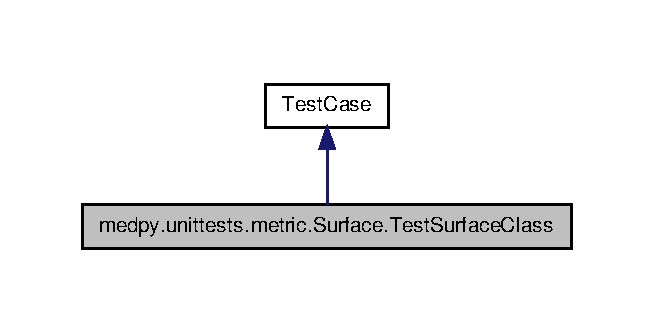
\includegraphics[width=314pt]{classmedpy_1_1unittests_1_1metric_1_1Surface_1_1TestSurfaceClass__inherit__graph}
\end{center}
\end{figure}


Collaboration diagram for medpy.unittests.metric.Surface.TestSurfaceClass:\nopagebreak
\begin{figure}[H]
\begin{center}
\leavevmode
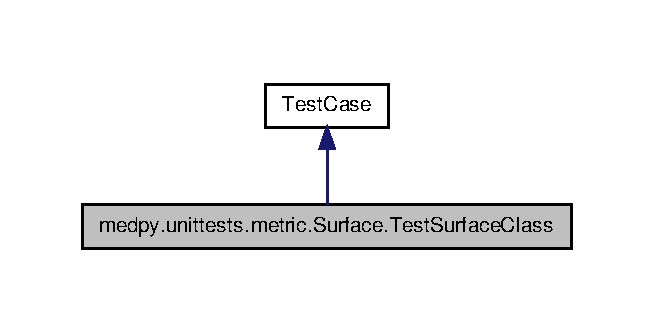
\includegraphics[width=314pt]{classmedpy_1_1unittests_1_1metric_1_1Surface_1_1TestSurfaceClass__coll__graph}
\end{center}
\end{figure}
\subsection*{Public Member Functions}
\begin{DoxyCompactItemize}
\item 
\hypertarget{classmedpy_1_1unittests_1_1metric_1_1Surface_1_1TestSurfaceClass_af6f10b41351cbd146f2af334e7a7c661}{
def {\bfseries setUp}}
\label{classmedpy_1_1unittests_1_1metric_1_1Surface_1_1TestSurfaceClass_af6f10b41351cbd146f2af334e7a7c661}

\item 
\hypertarget{classmedpy_1_1unittests_1_1metric_1_1Surface_1_1TestSurfaceClass_ae5faa8aa316ad7802013651f0b0d534d}{
def {\bfseries test\_\-Initialization}}
\label{classmedpy_1_1unittests_1_1metric_1_1Surface_1_1TestSurfaceClass_ae5faa8aa316ad7802013651f0b0d534d}

\item 
\hypertarget{classmedpy_1_1unittests_1_1metric_1_1Surface_1_1TestSurfaceClass_a030ba4445f3120543addea4788eba988}{
def {\bfseries test\_\-ComputeContour}}
\label{classmedpy_1_1unittests_1_1metric_1_1Surface_1_1TestSurfaceClass_a030ba4445f3120543addea4788eba988}

\item 
\hypertarget{classmedpy_1_1unittests_1_1metric_1_1Surface_1_1TestSurfaceClass_a1ed8d77fce82fea4ff666ee97294b9f1}{
def {\bfseries test\_\-GetMaximumSymmetricSurfaceDistance}}
\label{classmedpy_1_1unittests_1_1metric_1_1Surface_1_1TestSurfaceClass_a1ed8d77fce82fea4ff666ee97294b9f1}

\item 
\hypertarget{classmedpy_1_1unittests_1_1metric_1_1Surface_1_1TestSurfaceClass_a4b0285c8ac4cec38d8aded035d3e3e95}{
def {\bfseries test\_\-GetAverageSymmetricSurfaceDistance}}
\label{classmedpy_1_1unittests_1_1metric_1_1Surface_1_1TestSurfaceClass_a4b0285c8ac4cec38d8aded035d3e3e95}

\item 
\hypertarget{classmedpy_1_1unittests_1_1metric_1_1Surface_1_1TestSurfaceClass_af3f9d8b8f2d58af9f363be38b3a53e44}{
def {\bfseries test\_\-GetRootMeanSquareSymmetricSurfaceDistance}}
\label{classmedpy_1_1unittests_1_1metric_1_1Surface_1_1TestSurfaceClass_af3f9d8b8f2d58af9f363be38b3a53e44}

\end{DoxyCompactItemize}


\subsection{Detailed Description}


Definition at line 23 of file Surface.py.



The documentation for this class was generated from the following file:\begin{DoxyCompactItemize}
\item 
/home/omaier/Programming/Python/medpy/src/medpy/unittests/metric/Surface.py\end{DoxyCompactItemize}

\hypertarget{classmedpy_1_1unittests_1_1metric_1_1Volume_1_1TestVolumeClass}{
\section{medpy.unittests.metric.Volume.TestVolumeClass Class Reference}
\label{classmedpy_1_1unittests_1_1metric_1_1Volume_1_1TestVolumeClass}\index{medpy::unittests::metric::Volume::TestVolumeClass@{medpy::unittests::metric::Volume::TestVolumeClass}}
}


Inheritance diagram for medpy.unittests.metric.Volume.TestVolumeClass:\nopagebreak
\begin{figure}[H]
\begin{center}
\leavevmode
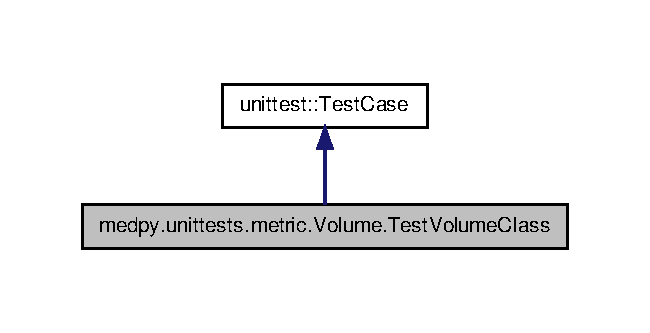
\includegraphics[width=312pt]{classmedpy_1_1unittests_1_1metric_1_1Volume_1_1TestVolumeClass__inherit__graph}
\end{center}
\end{figure}


Collaboration diagram for medpy.unittests.metric.Volume.TestVolumeClass:\nopagebreak
\begin{figure}[H]
\begin{center}
\leavevmode
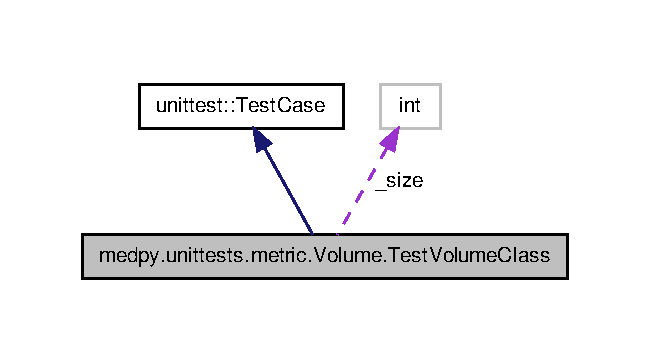
\includegraphics[width=312pt]{classmedpy_1_1unittests_1_1metric_1_1Volume_1_1TestVolumeClass__coll__graph}
\end{center}
\end{figure}
\subsection*{Public Member Functions}
\begin{DoxyCompactItemize}
\item 
\hypertarget{classmedpy_1_1unittests_1_1metric_1_1Volume_1_1TestVolumeClass_a2f291c94d8dd72c2eafd5bfddd2eab5c}{
def {\bfseries test\_\-GetVolumetricOverlapError}}
\label{classmedpy_1_1unittests_1_1metric_1_1Volume_1_1TestVolumeClass_a2f291c94d8dd72c2eafd5bfddd2eab5c}

\item 
\hypertarget{classmedpy_1_1unittests_1_1metric_1_1Volume_1_1TestVolumeClass_a9a007c447b6c90567f15f4a601a1aff7}{
def {\bfseries test\_\-GetRelativeVolumeDifference}}
\label{classmedpy_1_1unittests_1_1metric_1_1Volume_1_1TestVolumeClass_a9a007c447b6c90567f15f4a601a1aff7}

\end{DoxyCompactItemize}


\subsection{Detailed Description}


Definition at line 23 of file Volume.py.



The documentation for this class was generated from the following file:\begin{DoxyCompactItemize}
\item 
/home/omaier/Programming/Python/medpy/src/medpy/unittests/metric/Volume.py\end{DoxyCompactItemize}

\hypertarget{classmedpy_1_1metric_1_1volume_1_1Volume}{
\section{medpy.metric.volume.Volume Class Reference}
\label{classmedpy_1_1metric_1_1volume_1_1Volume}\index{medpy::metric::volume::Volume@{medpy::metric::volume::Volume}}
}


Computes different volume metrics between two 3D-\/images contain each a binary object.  




Inheritance diagram for medpy.metric.volume.Volume:\nopagebreak
\begin{figure}[H]
\begin{center}
\leavevmode
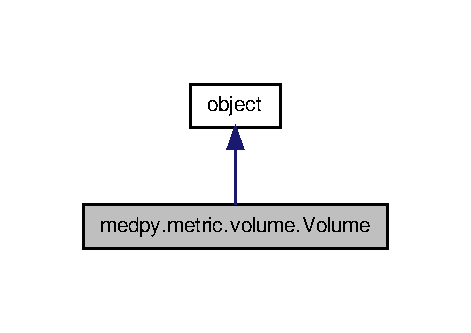
\includegraphics[width=226pt]{classmedpy_1_1metric_1_1volume_1_1Volume__inherit__graph}
\end{center}
\end{figure}


Collaboration diagram for medpy.metric.volume.Volume:\nopagebreak
\begin{figure}[H]
\begin{center}
\leavevmode
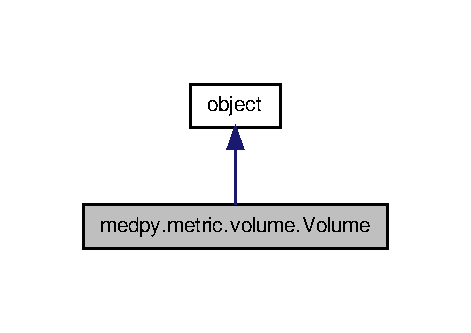
\includegraphics[width=226pt]{classmedpy_1_1metric_1_1volume_1_1Volume__coll__graph}
\end{center}
\end{figure}
\subsection*{Public Member Functions}
\begin{DoxyCompactItemize}
\item 
def \hyperlink{classmedpy_1_1metric_1_1volume_1_1Volume_ad5c463235786414fc4ff2b2157995722}{\_\-\_\-init\_\-\_\-}
\begin{DoxyCompactList}\small\item\em Initialize the class with two binary images whose 0 values are considered to be background voxels and the 1 values foreground. \end{DoxyCompactList}\item 
def \hyperlink{classmedpy_1_1metric_1_1volume_1_1Volume_ac1778f1c2a896936dc587e43da5dc6ab}{GetRelativeVolumeDifference}
\begin{DoxyCompactList}\small\item\em Returns the relative volume difference between two shapes defined by the non-\/background voxels of in the binary images. \end{DoxyCompactList}\item 
def \hyperlink{classmedpy_1_1metric_1_1volume_1_1Volume_a0b56a5881f4587543d6e12457700ad61}{GetVolumetricOverlapError}
\begin{DoxyCompactList}\small\item\em Returns the volumetric overlap error between two shapes defined by the non-\/background voxels of in two binary images. \end{DoxyCompactList}\item 
\hypertarget{classmedpy_1_1metric_1_1volume_1_1Volume_a71ceaa45f8287f4f1f811f2589218454}{
def \hyperlink{classmedpy_1_1metric_1_1volume_1_1Volume_a71ceaa45f8287f4f1f811f2589218454}{GetMaskSize}}
\label{classmedpy_1_1metric_1_1volume_1_1Volume_a71ceaa45f8287f4f1f811f2589218454}

\begin{DoxyCompactList}\small\item\em Computes the mask objects size if not yet done and returns it. \end{DoxyCompactList}\item 
\hypertarget{classmedpy_1_1metric_1_1volume_1_1Volume_ae2437de6098136c28250c9bdacc9a235}{
def \hyperlink{classmedpy_1_1metric_1_1volume_1_1Volume_ae2437de6098136c28250c9bdacc9a235}{GetReferenceSize}}
\label{classmedpy_1_1metric_1_1volume_1_1Volume_ae2437de6098136c28250c9bdacc9a235}

\begin{DoxyCompactList}\small\item\em Computes the reference objects size if not yet done and returns it. \end{DoxyCompactList}\item 
\hypertarget{classmedpy_1_1metric_1_1volume_1_1Volume_a2740aebb1d3a30e50a4facb355bcf1a4}{
def \hyperlink{classmedpy_1_1metric_1_1volume_1_1Volume_a2740aebb1d3a30e50a4facb355bcf1a4}{GetIntersectionSize}}
\label{classmedpy_1_1metric_1_1volume_1_1Volume_a2740aebb1d3a30e50a4facb355bcf1a4}

\begin{DoxyCompactList}\small\item\em Computes the two objects intersection size if not yet done and returns it. \end{DoxyCompactList}\item 
\hypertarget{classmedpy_1_1metric_1_1volume_1_1Volume_ae8d79f3cbe067d886c4d1519c100a33a}{
def \hyperlink{classmedpy_1_1metric_1_1volume_1_1Volume_ae8d79f3cbe067d886c4d1519c100a33a}{GetUnionSize}}
\label{classmedpy_1_1metric_1_1volume_1_1Volume_ae8d79f3cbe067d886c4d1519c100a33a}

\begin{DoxyCompactList}\small\item\em Computes the two objects union size if not yet done and returns it. \end{DoxyCompactList}\end{DoxyCompactItemize}


\subsection{Detailed Description}
Computes different volume metrics between two 3D-\/images contain each a binary object. 

Beside this provides a number of statistics of the two images.

Metrics defined in: Heimann, T.; van Ginneken, B.; Styner, M.A.; Arzhaeva, Y.; Aurich, V.; Bauer, C.; Beck, A.; Becker, C.; Beichel, R.; Bekes, G.; Bello, F.; Binnig, G.; Bischof, H.; Bornik, A.; Cashman, P.; Ying Chi; Cordova, A.; Dawant, B.M.; Fidrich, M.; Furst, J.D.; Furukawa, D.; Grenacher, L.; Hornegger, J.; Kainmuller, D.; Kitney, R.I.; Kobatake, H.; Lamecker, H.; Lange, T.; Jeongjin Lee; Lennon, B.; Rui Li; Senhu Li; Meinzer, H.-\/P.; Nemeth, G.; Raicu, D.S.; Rau, A.-\/M.; van Rikxoort, E.M.; Rousson, M.; Rusko, L.; Saddi, K.A.; Schmidt, G.; Seghers, D.; Shimizu, A.; Slagmolen, P.; Sorantin, E.; Soza, G.; Susomboon, R.; Waite, J.M.; Wimmer, A.; Wolf, I.; , \char`\"{}Comparison and Evaluation of Methods for Liver Segmentation From CT Datasets,\char`\"{} Medical Imaging, IEEE Transactions on , vol.28, no.8, pp.1251-\/1265, Aug. 2009 doi: 10.1109/TMI.2009.2013851 \begin{DoxyVerb}The mask image as scipy array.\end{DoxyVerb}
 

Definition at line 32 of file volume.py.



\subsection{Constructor \& Destructor Documentation}
\hypertarget{classmedpy_1_1metric_1_1volume_1_1Volume_ad5c463235786414fc4ff2b2157995722}{
\index{medpy::metric::volume::Volume@{medpy::metric::volume::Volume}!\_\-\_\-init\_\-\_\-@{\_\-\_\-init\_\-\_\-}}
\index{\_\-\_\-init\_\-\_\-@{\_\-\_\-init\_\-\_\-}!medpy::metric::volume::Volume@{medpy::metric::volume::Volume}}
\subsubsection[{\_\-\_\-init\_\-\_\-}]{\setlength{\rightskip}{0pt plus 5cm}def medpy.metric.volume.Volume.\_\-\_\-init\_\-\_\- (
\begin{DoxyParamCaption}
\item[{}]{self, }
\item[{}]{mask, }
\item[{}]{reference, }
\item[{}]{mask\_\-offset = {\ttfamily \mbox{[}0}, }
\item[{}]{reference\_\-offset = {\ttfamily \mbox{[}0}}
\end{DoxyParamCaption}
)}}
\label{classmedpy_1_1metric_1_1volume_1_1Volume_ad5c463235786414fc4ff2b2157995722}


Initialize the class with two binary images whose 0 values are considered to be background voxels and the 1 values foreground. 


\begin{DoxyParams}{Parameters}
{\em mask,:} & mask as an scipy array (3D image) \\
\hline
{\em reference,:} & reference as an scipy array (3D image) \\
\hline
{\em mask\_\-offset,:} & offset of the mask array to 0,0,0-\/origin \\
\hline
{\em mask\_\-offset,:} & offset of the reference array to 0,0,0-\/origin \\
\hline
\end{DoxyParams}


Definition at line 62 of file volume.py.



\subsection{Member Function Documentation}
\hypertarget{classmedpy_1_1metric_1_1volume_1_1Volume_ac1778f1c2a896936dc587e43da5dc6ab}{
\index{medpy::metric::volume::Volume@{medpy::metric::volume::Volume}!GetRelativeVolumeDifference@{GetRelativeVolumeDifference}}
\index{GetRelativeVolumeDifference@{GetRelativeVolumeDifference}!medpy::metric::volume::Volume@{medpy::metric::volume::Volume}}
\subsubsection[{GetRelativeVolumeDifference}]{\setlength{\rightskip}{0pt plus 5cm}def medpy.metric.volume.Volume.GetRelativeVolumeDifference (
\begin{DoxyParamCaption}
\item[{}]{self}
\end{DoxyParamCaption}
)}}
\label{classmedpy_1_1metric_1_1volume_1_1Volume_ac1778f1c2a896936dc587e43da5dc6ab}


Returns the relative volume difference between two shapes defined by the non-\/background voxels of in the binary images. 

The relative volume distance of 0 means that the volumes are identical. Note that this doesn't apply that the shapes are identical or overlap at all. The result is given as signed number \mbox{[}-\/100,+100\mbox{]} to indicate over-\/ or under-\/segmentation. Warning: Can produce values greater than -\//+100 if the difference in volume exceeds 50\%. Positive values means that the mask volume is too big, a negative value that it is too small.

Warning: This measure is not actually a metric, as it is not symmetric.

Metric definition: The relative volume difference between two sets of voxels $S(A)$ and $S(b)$ is given in percent and defined as: \[ 100 * \frac{|A - B|}{|B|} \] 

Definition at line 93 of file volume.py.

\hypertarget{classmedpy_1_1metric_1_1volume_1_1Volume_a0b56a5881f4587543d6e12457700ad61}{
\index{medpy::metric::volume::Volume@{medpy::metric::volume::Volume}!GetVolumetricOverlapError@{GetVolumetricOverlapError}}
\index{GetVolumetricOverlapError@{GetVolumetricOverlapError}!medpy::metric::volume::Volume@{medpy::metric::volume::Volume}}
\subsubsection[{GetVolumetricOverlapError}]{\setlength{\rightskip}{0pt plus 5cm}def medpy.metric.volume.Volume.GetVolumetricOverlapError (
\begin{DoxyParamCaption}
\item[{}]{self}
\end{DoxyParamCaption}
)}}
\label{classmedpy_1_1metric_1_1volume_1_1Volume_a0b56a5881f4587543d6e12457700ad61}


Returns the volumetric overlap error between two shapes defined by the non-\/background voxels of in two binary images. 

The volumetric overlap error is 0 for a perfect match and 100 if the two shapes don't overlap at all.

Metric definition: The volumetric overlap error between two sets of voxels $S(A)$ and $S(b)$ is given in percent and defined as: \[ 100 * \left( 1 - \frac{|A\cap B|}{|A\cup B|} \right) \] 

Definition at line 118 of file volume.py.



The documentation for this class was generated from the following file:\begin{DoxyCompactItemize}
\item 
/home/omaier/Programming/Python/medpy/src/medpy/metric/volume.py\end{DoxyCompactItemize}

\hypertarget{classmedpy_1_1filter_1_1Watershed_1_1Watershed}{
\section{medpy.filter.Watershed.Watershed Class Reference}
\label{classmedpy_1_1filter_1_1Watershed_1_1Watershed}\index{medpy::filter::Watershed::Watershed@{medpy::filter::Watershed::Watershed}}
}


Inheritance diagram for medpy.filter.Watershed.Watershed:\nopagebreak
\begin{figure}[H]
\begin{center}
\leavevmode
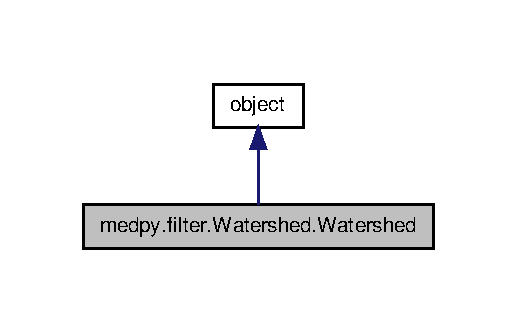
\includegraphics[width=248pt]{classmedpy_1_1filter_1_1Watershed_1_1Watershed__inherit__graph}
\end{center}
\end{figure}


Collaboration diagram for medpy.filter.Watershed.Watershed:\nopagebreak
\begin{figure}[H]
\begin{center}
\leavevmode
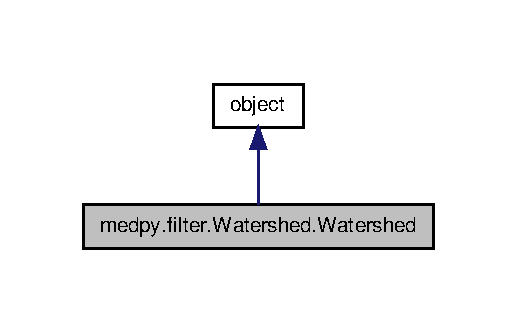
\includegraphics[width=248pt]{classmedpy_1_1filter_1_1Watershed_1_1Watershed__coll__graph}
\end{center}
\end{figure}


\subsection{Detailed Description}


Definition at line 22 of file Watershed.py.



The documentation for this class was generated from the following file:\begin{DoxyCompactItemize}
\item 
/home/loli/Programming/Python/MedPy/src/medpy/filter/Watershed.py\end{DoxyCompactItemize}

\printindex
\end{document}
